%
% You may wish to use some of the following options of the iitthesis
% package:
%
% fullpageDraft      avoid the margins necessary for proper binding and
%   just view or print a draft.
% beforeDefense      make the personal acknowledgements invisible;
%   use this to print the copies you submit initially to the grad school
%   for sending to the opponent panel, i.e. thesis readers (who shouldn't
%   see those parts). For the final submission, after having successfully
%   defended - drop this option.
% noabbrevs          avoid generation of a notation & abbreviations list
%
% Additionally, you must specify the degree for which you're writing
% your thesis (MSc/PhD/MArch etc.)
%
\documentclass[PhD]{misc/iitthesis}

% Definitions of info fields for the thesis - subject, advisor,
% faculty, acknowledgements, etc. etc. The thesis-fields file 
% contains Hebrew text, and should use the UTF-8 character set
% encoding (not iso-8859-8-i or windows codepage 1255).
% This file contains definitions of various fields used
% in various places throughout the thesis (in the title
% pages mostly). Whatever isn't define here has some
% default (and usually irrelevant) text.

\authorEnglish{Eytan Singher}
\authorHebrew{איתן סינגר}

\titleEnglish{Effective Automatic Deductive Reasoning Using Equality Saturation}
\titleHebrew{היסק דדוקטיבי אוטומטי אפאקטיבי באמצעות רוויון שוויונות}

\disciplineEnglish{Computer Science}
\disciplineHebrew{מדעי המחשב}

\supervisionEnglish{This research was carried out under the supervision of Prof.~Shachar Itzhaky, in the Faculty of Computer Science.}
\supervisionHebrew{המחקר בוצע בהנחייתו של פרופסור שחר יצחקי, בפקולטה למדעי המחשב.}

\GregorianDateEnglish{July 2024}
\GregorianDateHebrew{יולי \textenglish{2024}}
\JewishDateEnglish{Sivan 5784}
\JewishDateHebrew{סיוון התשפ"ד}

%\financialAcknowledgementEnglish{The Technion's funding of this research is hereby acknowledged.}
%\financialAcknowledgementHebrew{הכרת תודה מסורה לטכניון על מימון מחקר זה.}

\publicationInfoEnglish{
Some results in this thesis have been published as articles by the author and research collaborators in conferences and journals during the course of the author's doctoral research period, the most up-to-date versions of which being:

\butcheredbibliography{front/pubinfo.bib}
}

\publicationInfoHebrew{%
(התייחסות לפרסומים, שמופיעה להלן, הינה הכרחית לפי תקנות ביה"ס ללימודי מוסמכים; כמובן שיש למחוק את ההערה הזו שבסוגריים... תוכן זה נמצאה בקובץ \textenglish{\texttt{thesis-fields.tex}}. הרשומות לצורך רשימת הפרסומים הינן רשומות \textenglish{BibTeX}, נפרדות מן הרשומות בביבליוגרפיה העיקרית של המסמך: עליך לשים אותן בקובץ \textenglish{\texttt{front/pubinfo.bib}}; הקפיד/י שהתוויות שלהם יהיו שונות מתוויות הרשומות בביליוגרפיה העיקרית. רשום/י אותם בסדר בהם תרצה/י שיופיעו ברשימה --- שכן הן לא ימוינו. כן שים/י לב שייתכן שיהיה צורך להדר את המסמך פעם או פעמיים נוספות עד שהרשימה אכן תופיע כראוי.)

חלק מן התוצאות בחיבור זה פורסמו כמאמרים מאת המחבר ושותפיו למחקר בכנסים ובכתבי-עת במהלך תקופת מחקר הדוקטורט של המחבר, אשר גרסאותיהם העדכניות ביותר הינן:%

\begin{otherlanguage}{english}%
\butcheredbibliography{front/pubinfo.bib}
\end{otherlanguage}%
}

\addbibresource{back/general.bib}
% \thesisbibstyle{trad-alpha}


% Personal acknowledgements (are only used for the post-exam
% version)
\personalAcknowledgementEnglish{
I would like to thank my advisor, Shachar Itzhaky, for being there, and giving guidance and advice when necessary. 

Add any thank-yous, acknowledgements, personal comments you wish to make here (in \texttt{personal-acks.tex}).

Note that this acknowledgements section only gets printed in the post-exam version of the thesis (i.e. if you leave out the \texttt{beforeDefense} option to your document class in \texttt{thesis.tex}.)
}

\personalAcknowledgementHebrew{

אני רוצה להודות למנחה שלי, להוריי, לחבריי, וכו' וכו'.

אפשר להוסיף עוד תודות והערות אישיות כאן.

שים/י לב: קטע זה של תודות מודפס בפועל רק בגרסת החיבור שלאחר-הבחינה (הווה אומר רק אם הסרת את האפשרות \textenglish{\texttt{beforeDefense}} מן האפשרויות המועברות ל-\textenglish{\texttt{document class}} בקובץ \textenglish{\texttt{thesis.tex}}.)
}


% A separate file for the abstract - in English and in Hebrew, so
% you must make sure it's also in the UTF-8 character set encoding.
%
\input{front/abstract}

% Comment this if you do not want a list of abbreviations and acronyms
% (if you have used the noabbrevs option).
% Use this file to create "glossary entries" for abbreviations and acronyms,
% and other notation. The entries defined here don't necessarily have to be 
% used in the thesis (but then you have to decide whether or not to display
% the unused entries).

% For this file to compile (and the example text in the main/prelims.tex file),
% the package glossaries-extra is required. It is automatically included unless
% the noabbrevs class option is used.

% The following will alter the style for typesetting abbreviations when using 
% the \gls command. Note you can also use multiple styles by categorizing 
% abbreviations; see the documentation for the glossaries-extras package at:
% https://ctan.org/pkg/glossaries-extra
%
%\setabbreviationstyle[acronym]{long-short-sc}
%
% If you're wondering why we're setting the seemingly-redundant "notation 
% category", that's a hack discussed here:
% https://tex.stackexchange.com/q/630541/5640 

\newacronym[%
  category=notation-category,%
  description=``The Senate and People of Rome'']% The description does not appear anywhere by default
  {spqr}% the key of the acronym (used with the \gls command for example)
  {SPQR}% the short form of the acronym
  {Senātus Populusque Rōmānus}% the long form of the acronym

\newacronym[%
  category=notation-category,%
description=A technology used in data storage devices]%
  {smart}{SMART}{Self-Monitoring, Analysis and Reporting Technology}

\newacronym[%
  category=notation-category,%
  description=to build or produce something{,} rather than purchasing it ready-made or paying someone to make it]%
  {DIY}{DIY}{do it yourself}

\newacronym[%
  category=notation-category,%
  description=a four-letter acronym]
  {etla}
  {ETLA}
  {extended three-letter acronym}

\newabbreviation[%
  type=notation,%
  category=notation-category,%
  description=]% This abbreviation has no description; only the abbreviation and the unabbreviated form will be shown
  {aut}{Aut}{Automorphism group}

\newglossaryentry{symb:c}{%
  type=notation,%
  category=notation-category,%
  name=$c$,%
  description=the speed of light%
}

\newglossaryentry{symb:a-b-closed}{%
  type=notation,%
  category=notation-category,%
  name=\ensuremath{a \pm b},%
  description=the closed interval \ensuremath{\left[a-b,a+b\right]}%
}

\newglossaryentry{supercali}{%
  type=notation,%
  category=notation-category,%
  name=supercalifragilisticexpialidocious,
  description=%
    Atoning for being educable through delicate beauty;
    Something to say when you have nothing to say.}

% --------------------------------

% Commands below will control the behavior/appearance of the list of abbreviations and acronyms

% Uncomment this command to have _all_ abbreviations and acronyms defined
% in this file appear in the final list - rather than just the ones you
% use in the thesis
%\keepUnusedAbbreviations
\newabbreviation[%
  type=notation,
  category=notation-category,%
  description={Automated reasoning technique that compactly represents sets of equivalent expressions}]%
  {eqsat}{EqSat}{Equality Saturation}

\newabbreviation[%
  type=notation,
  category=notation-category,%
  description={Data structure that efficiently represents sets of equivalent expressions}]%
  {egraphs}{e-graphs}{Equality Graphs}

\newabbreviation[%
  type=notation,
  category=notation-category,%
  description={Equality Classes}]%
  {eclasses}{e-classes}{Equality Classes}

\newabbreviation[%
  type=notation,
  category=notation-category,%
  description={Theory exploration system leveraging equality saturation}]%
  {thesy}{TheSy}{Theory Synthesizer}

\newabbreviation[%
  type=notation,
  category=notation-category,%
  description={Extension to e-graphs for efficient conditional reasoning}]%
  {cegraph}{Colored E-graph}{Colored Equality Graph}

\newacronym[%
  category=notation-category,%
  description={Equality saturation-based automated reasoning tool for proof assistants}]%
  {les}{LES}{\emph{Lightweight Equality Saturation}}

\newacronym[%
  category=notation-category,%
  description={Interactive Theorem Prover}]%
  {itp}{ITP}{Interactive Theorem Prover}

\newacronym[%
  category=notation-category,%
  description={Automated Theorem Prover}]%
  {atp}{ATP}{Automated Theorem Prover}

\newacronym[%
  category=notation-category,%
  description={First-Order Logic}]%
  {fol}{FOL}{First-Order Logic}

\newacronym[%
  category=notation-category,%
  description={Higher-Order Logic}]%
  {hol}{HOL}{Higher-Order Logic}

\newacronym[%
  category=notation-category,%
  description={Calculus of Inductive Constructions}]%
  {cic}{CIC}{Calculus of Inductive Constructions}

\newacronym[%
  category=notation-category,%
  description={Pure Type System}]%
  {pts}{PTS}{Pure Type System}

\newacronym[%
  category=notation-category,%
  description={Proof Irrelevant Pure Type System}]%
  {pipts}{piPTS}{Proof Irrelevant Pure Type System}

\newacronym[%
  category=notation-category,%
  description={Equality-Program Expression Graphs}]%
  {epeg}{E-PEG}{Equality-Program Expression Graphs}

\newglossaryentry{symb:congruence}{%
  type=notation,%
  category=notation-category,%
  name=\ensuremath{\sim},%
  description={Congruence relation in e-graphs}%
}

\newglossaryentry{symb:forall}{%
  type=notation,%
  category=notation-category,%
  name=\ensuremath{\forall},%
  description={Universal quantification}%
}

\newglossaryentry{symb:exists}{%
  type=notation,%
  category=notation-category,%
  name=\ensuremath{\exists},%
  description={Existential quantification}%
}

\newglossaryentry{symb:implies}{%
  type=notation,%
  category=notation-category,%
  name=\ensuremath{\Rightarrow},%
  description={Logical implication}%
}

\newglossaryentry{symb:iff}{%
  type=notation,%
  category=notation-category,%
  name=\ensuremath{\Leftrightarrow},%
  description={If and only if (logical equivalence)}%
}

\newglossaryentry{symb:eclass}{%
  type=notation,%
  category=notation-category,%
  name=\ensuremath{[e]},%
  description={The equality class (e-class) containing the expression $e$ in an e-graph. It represents all expressions that are known to be equivalent to $e$}%
}

\newglossaryentry{rewrite-rule}{%
  type=notation,%
  category=notation-category,%
  name={\ensuremath{\mathcal{R} = t_1 \overset{.\,}{\rightarrow} t_2}},%
  symbol={\ensuremath{\mathcal{R} = t_1 \rwto t_2}},%
  description={A rewrite rule $\mathcal{R}$ representing a universally quantified formula of the form $\forall x_1, \ldots, x_n.~t_1 \implies t_2$,
    and all free variables are implicitly quantified.}%
}

\newglossaryentry{context-filling}{%
  type=notation,%
  category=notation-category,%
  name={\ensuremath{C[t]}},%
  description={Context filling operation, where $C$ is a context (a term with a single hole) and $t$ is the term used to fill the hole}%
}

\newglossaryentry{substitution}{%
  type=notation,%
  category=notation-category,%
  name={\ensuremath{t\sigma}},%
  description={Substitution operation, where $\sigma$ is a mapping from variables to terms, applied to replace variables in the term $t$}%
}

\newglossaryentry{metavariable}{%
  type=notation,%
  category=notation-category,%
  name={\ensuremath{?v_i}},%
  description={A metavariable, represented as $?v_i$, is used as a hole in a pattern. 
  A pattern is a term with zero or more such holes.}%
}

\newacronym[%
  category=notation-category,%
  description={Rules that specify how to transform one term into another equivalent term in a formal system.}]%
  {rr}{r.r.}{\emph{rewrite rules}}

  \newacronym[%
  category=notation-category,%
  description={A rewrite rule that includes a precondition. It takes the form $\phi \Rightarrow t_1 \rwto t_2$, where $\phi$ is a condition that must be satisfied for the rule to be applied.}]%
  {crr}{c.r.r.}{\emph{conditional rewrite rule}}

  \newacronym[%
  category=notation-category,%
  description={Symbolic Observational Equivalence}]%
  {soe}{SOE}{\emph{Symbolic Observational Equivalence}}

\newacronym[%
  category=notation-category,%
  description={A composite data type defined by specifying a collection of constructors, each with its own arguments.}]%
  {adt}{ADT}{Algebraic Data Type}

\newacronym[%
  category=notation-category,%
  description={The use of computer systems to assist in the creation, modification, analysis, or optimization of a design.}]%
  {cad}{CAD}{Computer-Aided Design}

% Additional machinery relevant to any thesis
% (it's not part of the document class because it's not absolutely
% necessary and not everyone might like it)
% General-purpose definitions and inclusions
% you are using in any document 
% (regardless of its class and style files used),
% e.g. package uses:

%\usepackage{xspace}

% and macros/command defintions:

%\newcommand{\complexityclass}[1]{{\bf #1}\xspace}
%\newcommand{\NPTIME}{\complexityclass{NP}}

% For this template, we'll only have one single command,
% necessary for including graphics...
\usepackage{graphicx}% http://ctan.org/pkg/graphicx
\usepackage{cabin}  % sans-serif font

\usepackage{amssymb}
\usepackage{listings}
\usepackage[table]{xcolor}
\usepackage{hyperref}
\usepackage[normalem]{ulem}
\usepackage{mathtools}
\usepackage{comment}
\usepackage{xspace}
\usepackage{multirow}
\usepackage[rightcaption]{sidecap}
\usepackage[normalem]{ulem} % for \sout
\usepackage{enumitem}
\usepackage{relsize}
\usepackage[firstpage]{draftwatermark}
\usepackage[misc]{ifsym}

\usepackage{tikz}
\usetikzlibrary{arrows, positioning, fit, plotmarks}
\usepackage{tikzsymbols}
\usepackage{pgfplots}
\pgfplotsset{compat=1.16}
\usepackage{lipsum}

\usepackage{cleveref}
\usepackage{latexsym}
\usepackage{colortbl}
\usepackage{graphicx}
\usepackage{booktabs}
\usepackage[export]{adjustbox}
\usepackage{dcolumn}
\newif\iffinal
\newif\ifcomments
\commentstrue
% \finaltrue

\ifcomments
\newcommand\ES[1]{{\color{orange}[ES: #1]}}
\newcommand\SI[1]{{\color{purple}[SI: #1]}}
\else
\iffinal\else
\newcommand\ES[1]{{}}
\newcommand\SI[1]{{}}
\fi
\fi

\newcommand\eg{\textit{e.g.\@}\xspace}
\newcommand\Eg{\textit{E.g.\@}\xspace}
\newcommand\ie{\textit{i.e.\@}\xspace}
\newcommand\Ie{\textit{I.e.\@}\xspace}
\newcommand\vs{\textit{vs.\@}\xspace}

\newenvironment{myparagraph}[1]
    {\smallskip\noindent\textbf{#1}~~}{}


% For double blind submission
\newsavebox{\incog}
\sbox{\incog}{
  
\includegraphics[height=5mm,trim=10 10 10 10,clip]
       {thesy/img/Incognito.pdf}
}
\newcommand\incognito{\usebox{\incog}}

\newcommand\TheSy{{TheSy}\xspace}

% autoref configuration
\renewcommand*{\sectionautorefname}{Section}
\renewcommand*{\subsectionautorefname}{Subsection}

\newcommand\iterm[1]{{#1}}

% some operators
\newcommand\operatorstyle[1]{\textrm{\fontfamily{ptm}\selectfont#1}}
\DeclareMathOperator{\cons}{\operatorstyle{::}}
\DeclareMathOperator{\snoc}{\operatorstyle{:+}}
\DeclareMathOperator{\concat}{\operatorstyle{++}}

\newcommand{\lnil}{\mbox{\relscale{0.9}$[\,]$}}

\DeclareMathOperator{\maybeEq}{\overset{?}{\,=\,}}
\DeclareMathOperator{\maybeEqTiny}{\overset{\scriptscriptstyle ?}{\,=\,}}
\DeclareMathOperator{\eqdef}{~\widehat{=}~}

\newcommand\substInTerm[3]{#1\big[#2\big/\!#3\!\big]}

% specific notation
\newcommand\Lang{\mathcal{L}}
\newcommand\Vocab{\mathcal{V}}
\newcommand\Constr{\mathcal{C}}
\newcommand\Eqs{\mathcal{E}}
\newcommand\Rewrite{\mathcal{R}}
\newcommand\conjspace{\mathcal{S}_{EqCj}}
\DeclareMathOperator{\rwto}{\overset{.\,}{\rightarrow}}
\newcommand\Terms{\mathcal{T}}
\newcommand\Type{\tau}
\newcommand\Types{\mathcal{T_Y}}

\newcommand\RewriteRelation[2]{#1 \xrightarrow[]{\Rewrite} #2}
\newcommand\SRewriteRelation[2]{#1 \xleftrightarrow[]{\Rewrite\,} #2}
\newcommand\SRewriteRelationi[2]{#1 \xleftrightarrow[]{\Rewrite_i} #2}
\newcommand\RewriteSys{\{\Rewrite_i\}}%{G_\Rewrite}
\newcommand\ARewriteSysRelation[2]{#1 \xrightarrow[]{\RewriteSys} #2}
\newcommand\RewriteSysRelation[2]{#1 \xleftrightarrow[]{\RewriteSys} #2}

\newcommand\TRewriteSysRelationSymbol{\xleftrightarrow[]{\RewriteSys}^*}
\newcommand\TRewriteSysRelation[2]{{#1} \,\TRewriteSysRelationSymbol\! {#2}}
\newcommand\TRewriteSysRelationTiny[2]{{#1} \xleftrightarrow[]{\scriptscriptstyle\RewriteSys^*\!\!} {#2}}
\newcommand\TLRewriteSysRelation[2]{#1 {\xleftrightarrow[]{\RewriteSys}^*}\big|_\Terms #2}
\newcommand\RewriteSysRelationBounded[3]{#1 {~\xleftrightarrow[]{\RewriteSys}}^{\!(#3)} #2}
\newcommand\TRewriteSysRelationBounded[3]{#1 \underset{\Terms}{\xleftrightarrow[]{\RewriteSys}}^{\!(#3)} #2}
\newcommand\FV{\mathrm{FV}}
\newcommand\SymbolicExamples{SEs}
\newcommand\SERelation[2]{#1 \cong #2}

\newcommand\pholder[2]{\overset{\scriptscriptstyle #2}{\circ_{\mbox{\relscale{.6}$#1$}}}}  % OCD much?
\newcommand\Symexes[1]{\mathcal{S}^{#1}}
\newcommand\EquivRel{\mathcal{Q}}

\newcommand\ctor{\mathit{ctor}}
\DeclareMathOperator{\ltwf}{\sqsubset}

\newcommand\prvbyS{\overset{\scriptscriptstyle S}{\vdash}}
\newcommand\prvbySinline{\vdash^{^{\hspace{-.4em}S\hspace{-.2em}}}}

% functions that we love
\newcommand\treverse{\textrm{reverse}}
\newcommand\tfilter{\textrm{filter}}
\newcommand\tmap{\textrm{map}}
\newcommand\tfold{\textrm{fold}}
\newcommand\tsum{\textrm{sum}}
\newcommand\tlen{\textrm{len}}
\newcommand\tsucc{\textrm{succ}}
\newcommand\tswitch{\textrm{switch}}
\newcommand\ttreeflat{\textrm{flatten}}
\newcommand\ttreemap{\textrm{tmap}}
\newcommand\tid{\textrm{id}}
\newcommand\tdrop{\textrm{drop}}
\newcommand\ttake{\textrm{take}}
\newcommand\tmax{\funcname{max}}
\newcommand\tmin{\funcname{min}}
\newcommand\tissorted{\funcname{is\_sorted}}
\newcommand\tbinsearch{\funcname{bin\_search}}
\newcommand\tlfind{\funcname{find}}

\newcommand\tprim[1]{{\textsf{\itshape\relscale{.9}#1}}}
\newcommand\ttrue{\tprim{true}}
\newcommand\tfalse{\tprim{false}}
\newcommand\tforall{\tprim{all-true}}
\newcommand\texists{\tprim{any-true}}


\newcommand\trev{\textrm{rev}}  % short for reverse

% types (that we also love)
\newcommand\ttype[1]{{\textsf{\relscale{.9}#1}}}
\newcommand\tlist{\ttype{list}}
\newcommand\tbool{\ttype{bool}}
\newcommand\tnat{\ttype{nat}}

\newcommand\tkeyword[1]{\textrm{\color{blue!70!black}#1}}

\newcommand\tif{\tkeyword{if}}
\newcommand\tthen{\tkeyword{then}}
\newcommand\telse{\tkeyword{else}}
\newcommand\tmatch{\tkeyword{match}}
\newcommand\twith{\tkeyword{with}}

\lstset{basicstyle=\ttfamily}

% A bit of color
\newcommand\clrterm{\color{blue!65!green}}
\newcommand\clratom{\color{blue!60!green}}
\newcommand\clrsymex{\color{orange!40!red}}
\newcommand\clrhi{\color{red!70!black}}

\newcommand\cmptheories{\textsf{\color{violet!50!white}\smaller{\hspace{1pt}\%\hspace{1pt}}}}

\newcommand\funcname[1]{\textsf{\fontsize{8.5pt}{8pt}\selectfont#1}}
\newcommand\smallfuncname[1]{\textsf{\fontsize{7.5pt}{7pt}\selectfont#1}}

\newcommand\ecid[1]{\langle #1\rangle}

\newcommand\tsmallmax{\smallfuncname{max}}
\newcommand\tsmallmin{\smallfuncname{min}}

\newcommand\apifun[1]{\mathit{#1}}
\newcommand\tunion{\apifun{union}}
\newcommand\tfind{\apifun{find}}
\newcommand\tinsert{\apifun{insert}}
\newcommand\tmerge{\apifun{merge}}

\definecolor{olivegreen}{HTML}{3C8031}

\newcommand\croot{\ensuremath{\varnothing}\xspace}
\newcommand\cblue{{\color{blue}blue}\xspace}
\newcommand\cred{{\color{red}red}\xspace}
\newcommand\cgreen{{\color{olivegreen}green}\xspace}

\newcommand\tterm{\mathit{term}}
\newcommand\treg{\mathit{reg}}
\newcommand\tin{\mathit{in}}
\newcommand\tout{\mathit{out}}
\newcommand\trevpath{\mathit{reverse\_path}}
\newcommand\tcolor{\mathit{color}}
\newcommand\teclass{\mathit{eclass}}
\newcommand\tdescendants{\mathit{descendants}}
\newcommand\tminimal{\mathit{minimal}}

\newcommand\instr[1]{{\fontsize{9.5pt}{8pt}\selectfont\textsf{#1}}}
\newcommand\iinit{\instr{init}}
\newcommand\ibind{\instr{bind}}
\newcommand\icompare{\instr{compare}}
\newcommand\icheck{\instr{check}}
\newcommand\icontinue{\instr{continue}}
\newcommand\ijoin{\instr{join}}
\newcommand\iclrjmp{\instr{colored\_jump}}


\newcommand\congblue{{~\color{blue}\cong_{\mathrm{b}}\,\,}}
\newcommand\congred{{~\color{red}\cong_{\mathrm{r}}\,\,}}
\newcommand\conggreen{{~\color{olivegreen}\cong_{\mathrm{g}}\,\,}}

\newcommand\congbluesym{{\color{blue}\cong_{\mathrm{b}}}}


\newcommand\lowerred{{\color{red}_{\hspace{1pt}\mathrm{r}\hspace{0.5pt}}}}

\newcommand\eqid{\equiv_{\mathrm{id}}}

% because autoref does not work with the fmcad/IEEE class
\newcommand{\annexref}[1]{\hyperref[#1]{Appendix~\ref*{#1}}}

\usepackage{misc/iitthesis-extra}


\preparebutcheredbibliography{front/pubinfo.bib}

% Definitions useful for anything you write, which you also
% include in any articles, presentations, HW assignments and other
% documents. May contains macros for notation algebra, logic,
% calculus and other fields, as well as general shorthands and
% LaTeX tricks, and package use commands

% Definitions, settings and tweaks for this thesis specifically

\begin{document}

% Front Matter
% ------------

% The following command will typeset the outer cover page, the
% inner title page, the acknowledgements page, etc. - everything
% up to but not including the introduction
\makefrontmatter

% Main Matter
% ------------
%
% To conform to Technion regulations, the main matter should begin
% with an introduction (including a survey of relevant past work):
%
\chapter{Introduction}
\label{chap:intro}

% What is my story even?

% Deductive reasoning
% We have TheSy to create more deductions
% We have colored e-graphs to better apply deductions in exploratory settings
% We have a quick deductive prover as a proof of concept for better interactive verification. This is also somewhat exploratory for subproofs but we won't get there

% Equality satuartion pov
% Same as deductive but I can focus mainly on eqsat, so introduction will make more sense, and everything will be more focused
% I will need to start with equality saturation move quickly to deductive reasoning.
% Some background
% Then I can go into different approaches done in reasoning tasks I am interested in, and their accopanying equality saturation technique.
% Why is equality saturation succesful maybe quote.
% My specific techniques? Contributions

Deductive reasoning, a cornerstone of logical thought, forms the basis for many powerful techniques in automated reasoning systems. 
At its core, deductive reasoning involves drawing logical conclusions from a set of premises, applying general principles to specific instances. 
This approach has become instrumental in automatically proving properties of software systems, optimizing code, and discovering new mathematical truths.

Automatic deductive reasoning is mostly used for software development and validation.
As software systems have become increasingly complex, the importance of automated reasoning has grown significantly \cite{d2008survey}. 
Methods of optimization and verification are more crucial than ever, as software is embedded in critical infrastructure, from financial systems to healthcare devices.
Thus, automated reasoning techniques have been a center of attention for many years\footnote{But, attention is not all you need}. 
One of the fundamental approaches in this field is term rewriting. 
Term rewriting involves systematically replacing subterms of a formula with equivalent terms according to a set of rewrite rules. 
For example, in arithmetic, we might have a rule that states $a + b - b \rightarrow a$ where $a$ and $b$ are arbitrary terms. 
This rule would allow us to simplify expressions like $5 + (x\cdot y) - (x\cdot y)$ to just $5$.

While powerful, term rewriting faces several challenges:
\begin{enumerate}
    \item Termination: It's not always clear whether the rewriting process will terminate, especially with complex rule sets.
    \item Confluence: Even when termination is guaranteed, different rewriting sequences might lead to different normal forms, complicating reasoning about term equivalence.
    \item Information loss: Once a rewrite step is taken, the original term is typically discarded, potentially losing valuable information for later reasoning steps.
\end{enumerate}

To address some of these issues, techniques like the Knuth-Bendix completion algorithm \cite{knuthbendixcompletion} have been developed. 
This algorithm attempts to transform a set of equations into a confluent and terminating term rewriting system. 
That is, using the rewrite system on two provably equal terms will result in both terminating with the same normal form.
However, it doesn't fully solve the problem of information loss and can struggle with certain types of equations. 
For example, the commutativity of addition, $x + y \rightarrow y + x$, poses challenges for the Knuth-Bendix completion algorithm. 
If included directly as a rewrite rule, it can lead to non-termination \cite{kapur1985knuthintro}.

Equality saturation, a relatively new deductive reasoning technique that has emerged as a promising solution to many of these challenges \cite{eqsat}. 
It is based on e-graphs \cite{egg}, a data structure that can compactly represent a large set of equivalent terms.
In this context, a term is a symbolic expression that represents a mathematical expression or computation, typically composed of variables, constants, and function symbols, such as  $f(x+2)$ and $3 \cdot y^2$.
An easy way to think about e-graphs is as an extension of the union-find data structure to include congruence closure over terms.
In an e-graph, each node (called an e-class) represents a set of terms that are known to be equal.
Edges in the e-graph (somewhat confusingly called e-nodes) represent function applications.
For example, if we know that $a = b$ and $f(a) = c$, an e-graph could represent the terms $\{ a, b, c, f(a), f(b) \}$ with two e-classes $\{ e1, e2 \}$ and four e-nodes: $e1  = {a, b}$, $e2 = {f(|e1|), c}$.
Do note that $a$, $b$, and $c$ are treated as unary functions, and e-nodes are over e-classes, so we mark $|e1|$ to signify the parameter is the e-class $e1$.
The compact representation is based on shared subterms, so in the worse case no subterms are shared and no compaction is achieved.
However, an e-graph can also represent infinite expressions in a single e-class.
Let's take for example $x$ and $x + 0$.
Both will be in the same e-class $e$, but the e-node $|e| + 0$ is over any term represented by $e$, inductively leading to infinite terms.

Equality saturation employs e-graphs to build a compact representation of all possible rewrites of a given expression. 
Instead of applying rewrite rules sequentially and discarding intermediate results, equality saturation applies all possible rewrites simultaneously, storing the results in the e-graph. 
This approach allows for a more comprehensive exploration of the solution space without committing to a particular sequence of rewrites. 
The power of equality saturation has been demonstrated across various applications:

\paragraph{Program Optimization} Equality saturation has, originally and in later work, been used to discover complex code transformations that significantly improve performance \cite{eqsat}.
It's main advantage is the ability to choose global optimizations rather than local ones through classical heuristic rewriting.
Another instance, the TENSAT superoptimizer, uses equality saturation to find optimized tensor graphs \cite{tensat} which is important for the recent surge in deep learning tools and applications.
Similarly, the Herbie tool \cite{herbie} applies equality saturation achieving greatly improved accuracy of floating-point expressions.

\paragraph{Program Verification and Theorem Proving}
Equality saturation has also made significant strides in the domains of program verification and theorem proving. 
TheSy \cite{thesy}, which is part of the contributions of this thesis, leverages equality saturation for theory exploration, automatically discovering and proving new lemmas in mathematical theories.
In the realm of program analysis, the combination of abstract interpretation with equality saturation \cite{abstracteqsat} has shown promise in improving the precision and efficiency of static analysis tools. 
Equality saturation has been employed in fuzz testing of compilers as well. 
WASM Mutate \cite{arteaga2022wasm} to generate semantically equivalent mutations, aiding in testing and verification efforts of WASM compilers. 
Furthermore, an issue with using equality saturation (and its inherently applied congruence closure) was that proof traces could be difficult to verify. 
This is important, as usually verification systems like the Coq proof assistant \cite{Coq:manual} work on a small trusted core, and are often used to verify proofs from external tools \cite{armand2011modular, coqhammer}. 
The "Small Proofs from Congruence Closure" technique \cite{flatt2022small} demonstrates how equality saturation can be used to generate compact proofs from e-graphs, bridging the gap for equality saturation to be used in automated reasoning systems.

\paragraph{Program Synthesis} Equality saturation has proven to be particularly effective in program synthesis tasks due to its ability to compactly represent vast search spaces of potential programs.
This compact representation allows for efficient exploration of numerous program variants simultaneously.
For instance, the Babble synthesizer \cite{cao2023babble} leverages equality saturation to compress learned libraries of function, exploring a wide range of implementation choices in a single e-graph. 
In the domain of rewrite rule inference Ruler \cite{ruler} uses equality saturation to automatically discover new term rewriting rules from a set of input-output examples, effectively synthesizing program transformations. 
This approach has shown promise in automating the discovery of optimization rules for domain-specific languages. 
Furthermore, in the field of computer-aided design (CAD), the Szalinski tool \cite{nandi2020synthesizing} uses e-graphs to represent and manipulate CAD programs, enabling the synthesis of more abstract, parametric CAD models.

\bigskip

Despite these successes, the full potential of equality saturation in deductive reasoning remains to be explored. 
Several challenges persist:

\begin{itemize}
    \item While equality saturation is powerful for reasoning within a given theory, its effectiveness is limited to known equalities. Automatically discovering new theories or extending existing ones remains challenging.
    \item Handling conditions efficiently in the e-graph structure is not straightforward, limiting the applicability of equality saturation in scenarios involving complex logical conditions.
    \item Applicability for theorem provers is still an open problem. While rewriting systems were successfully employed in theorem provers, equality saturation has still not made a big footprint in the field.
\end{itemize}

This thesis aims to address these challenges and advance the field of deductive reasoning through novel applications and extensions of equality saturation. 

% -------------- Thesy -------------------------

\section{Expanding the Knowledge Base in Automated Reasoning}

In the context of automated deductive reasoning, \emph{knowledge base} refers to the set of facts, axioms, lemmas, and theorems that a system can use to derive new conclusions \cite{amlenat1977automated, thesy}.
For instance, in arithmetic reasoning, the knowledge base might include basic axioms like $x + y = y + x$ or more complex theorems like distribution of addition and multiplication $x * (y + z) = (x * y) + (x * z)$.

Automatic deduction based on a given knowledge base will fail when missing an important axiom.
For example, consider trying to find a proof for the equality $(y * 0) + x = x$.
Of course, if the knowledge base contains that equality directly then it is easy, it also can be deduced with a combination of axioms, $\forall y. y * 0 = 0$ and $\forall x. 0 + x = x$, it would be provable in two steps.
But, when the knowledge base would not contain relevant and matching axioms, the automatic deductive reasoning will fail.

For that reason, scientists devote a lot of effort into developing theories \cite{qedatlarge}.
To that end, the concept of automatically expanding this knowledge base, known as theory exploration, has been researched as well.
Theory exploration can be defined as the task of automatically discovering new, interesting, and provably correct mathematical knowledge from a given set of axioms and definitions.
Over the years, various approaches to theory exploration have been developed.

Starting already in the 1970s, researchers have developed systems for potentially increasing the knowledge base by heuristically discovering concepts (e.g. a circle, or prime numbers) and conjectures about them. \cite{amlenat1977automated,buchanan1981dendral}.
Generate-and-test methods, like the GRAPH THEORIST and HR systems \cite{epstein1988graphtheist,colton1999automatichr}, which generate conjectures, but then also attempt to prove them, thus improving usability.
All of these works depend greatly on the representation (or embedding) of the concepts to create conjectures and new concepts, due to the, often infinite, search space of conjectures to consider.

Newer methods attempt to deal with the search space explosion problem by using constrained synthesis and fast conjecture filtering, but do not attempt to recognize new concepts.
IsaCoSy \cite{JAR2010:Johanssonisacosy}, uses constraint-based synthesis to generate conjectures while trying to maintain completeness.
Other systems use templates as a heuristic to constrain or simplify conjecture generation \cite{einarsdottir2020template,ESA2012:Montanoschemebased,mccasland2006mathsaid}. 

More recent, and especially successful, approaches rely on equality relations as a means to compress the search space.
QuickSpec \cite{} uses observable equality (equality over a finite set of examples) as an equality relation.
However, observable equality suffers from two big issues.
First, it requires concrete examples to run, which QuickSpec partially solves by relying on the property testing. 
The second problem arises because observable equality may imply incorrect equalities leading to wrong conjectures, but further work, HipSpec \cite{hipster}, uses theorem provers on top of QuickSpec to circumvent correctness issues.
Additional work went into extending support for conditionals, improving runtime using schemes, and infinite streams \ES{cite into the infinite and speculate and roughspec (Template-based Theory Exploration)}, but the basic limitations of creating examples, especially for conditional conjectures, such as conjectures about concepts, remain.

Currently theory exploration still faces challenges when trying to fulfill all three goals at once:
\begin{itemize}
    \item Efficiency: Generating and testing a large number of potential theorems can be computationally expensive.
    \item Relevance: Many generated statements, while true, may not be useful or interesting.
    \item Completeness: Find all important theorems in a given domain. Especially challenging when considering conditional conjectures such as $sorted~list \implies min~list = head~list$
\end{itemize}

TheSy, one of the main contributions of this thesis, addresses these challenges by leveraging the power of equality saturation. 
Unlike previous approaches that rely on concrete evaluation or testing, TheSy uses symbolic reasoning to efficiently explore the space of potential theorems.
By representing a large space of equivalent expressions compactly in an e-graph, TheSy can simultaneously consider many potential lemmas. This approach allows for the discovery of non-obvious mathematical relationships that might be missed by more directed search strategies.
Moreover, TheSy's integration with equality saturation provides a symbiotic relationship: as new lemmas are discovered, they can be immediately incorporated into the e-graph, potentially enabling the discovery of even more complex relationships. This continuous expansion of the knowledge base can significantly enhance the reasoning capabilities of automated systems, allowing them to tackle increasingly complex problems.
In the following chapters, we will delve deeper into TheSy's architecture, algorithms, and its effectiveness in automated theory exploration, demonstrating how it advances the state of the art in expanding knowledge bases for automated reasoning systems.

% -------------- Contributions -------------

\section{Contributions and layout}

We present three main contributions:

\begin{enumerate}
    \item TheSy: A symbolic theory exploration system that leverages equality saturation to automatically discover and prove new mathematical conjectures. TheSy demonstrates how equality saturation can be used not just for reasoning within theories, but for expanding our mathematical knowledge.
    \item Colored E-graphs: An extension to the traditional e-graph structure that enables efficient handling of multiple assumptions, crucial for conditional reasoning. This contribution significantly expands the applicability of equality saturation to scenarios involving complex logical conditions.
    \item An Equality Saturation Prover for Pure Type Systems: This work demonstrates the applicability of equality saturation techniques to higher-order logic reasoning, opening up new possibilities for automated reasoning in advanced mathematical domains.
\end{enumerate}

Through these contributions, we aim to enhance the power and flexibility of automated deductive reasoning tools, opening new avenues for program verification, optimization, and mathematical discovery. By addressing key limitations of current equality saturation techniques, this work pushes the boundaries of what can be achieved in automated reasoning, potentially impacting a wide range of applications in computer science and mathematics.

As we delve deeper into each of these contributions in the subsequent chapters, we will explore how they build upon and extend the foundational concepts of equality saturation, and how they interact to create a more powerful and versatile framework for automated reasoning.

This expanded introduction provides more context about deductive reasoning, term rewriting, and equality saturation. It explains key concepts in more detail and gives concrete examples, making it more accessible to readers who might be less familiar with the field. It also more clearly sets up the challenges that your work addresses and the significance of your contributions.

Equality saturation, a relatively new deductive reasoning technique, has been successfully used in important tasks such as program optimization, program verification, and theorem proving. 
Based on e-graphs, equality saturation sets itself apart from traditional term rewriting systems by its compressed and non-destructive nature.
In the realm of program optimization, equality saturation was used for non-obvious code transformations that can significantly improved performance in various domains \ES{cite herbie, original eqsat, tensor optimizations, and others as are found}.
For program verification and theorem proving, equality saturation provides a flexible framework for deriving new mathematical insights and searching for proofs \cite{ruler, thesy, guidedeqsat, abstracteqsat}.


\begin{comment}
Please note that the \texttt{iitthesis} class has several options when you use it, such as:
\begin{itemize}
\item \texttt{fullpageDraft} to avoid the margins necessary for proper binding when you make the final print
\item \texttt{beforeDefense} makes the personal acknowledgements invisible; use this to print the copies you submit initially to the grad school for sending to the opponent panel, i.e. thesis readers (who shouldn't see those parts). For the final submission, after having successfully defended --- drop this option. 
\item \texttt{noabbrevs} no notation \& abbreviations list will be included in the thesis.
\end{itemize}

\subsection*{Hebrew font}

The \texttt{iitthesis} document class uses the David CLM font family for Hebrew text. CLM is a shorthand for ``Culmus'' (\texthebrew{קולמוס}) --- the name of a freely-available Hebrew font package. It may be bundled with your LaTeX distribution, or otherwise, must be available as system fonts. If you're missing the Culmus fonts, try adding an appropriate package from your LaTeX distribution or system distribution; alternatively, you might want to visit the Culmus project page at \url{http://culmus.sourceforge.net/} and download and install the fonts manually.    

\subsection*{Setting thesis meta-data and publication information}

The document class used to generate this document defines several commands you can use to set information  regarding your thesis, which is used in the title pages and elsewhere in the front matter.  Every (or almost every) command has an English and a Hebrew variant, with a \texttt{English} or \texttt{Hebrew} suffix to the command name. Examples:
\begin{itemize}
\item \verb|\titleHebrew|, \verb|\titleEnglish|
\item \verb|\authorHebrew|, \verb|\authorEnglish|
\item \verb|\JewishDateHebrew|, \verb|\JewishDateEnglish|
\item \verb|\GregorianDateHebrew|, \verb|\GregorianDateEnglish|
\item \verb|\publicationinfoHebrew|, \verb|\publicationinfoEnglish|
\end{itemize}

The file \texttt{misc/thesis-fields.tex} contains invocations of several such commands (some of them commented-out with \texttt{\%}), and some additional information about them.

\end{comment}




%
% and then cover:
% - The methods used in the research
% - The research results
% - Discussion and conclusions from the results
%
% but not necessarily with a specific chapter for each of them.
%
% Then you have your main chapters (although these might still
% include an initial chapter on technical preliminaries, experimental
% system setup, and/or a final chapter with summary, discussion and further
% research direction or questions)

\chapter{Preliminaries}
\label{chap:prelims}

A preliminaries chapter is not necessary, but it may be a good idea to use it for presenting your theoretical/mathematical framework in a more detailed and technical way than the introduction, and to perhaps establish some basic lemmata/observations common to multiple chapters of your thesis.

\section{Some section}

Let's define some concept we'll be using throughout the thesis.

\begin{definition}
The \emph{von Neumann model} of a computer, also known as the \emph{Princeton architecture} is an architecture for digital computers, which consists of a processing units, containing an ALU and processing registers; a control unit consisting of an instruction register and a program counter; a memory unit which stores both data and instructions; and input-and-output mechanisms.
\end{definition}

\section{Acronyms and abbreviations}

Your thesis will typically have a set of significant terms, abbreviations and acronyms. Technion guidelines mandate that you place a list of these at the beginning of your thesis; and that they be defined upon first use. And, indeed, if you followed read this sample thesis carefuly thus far you should have seen ``\nameref{chap:notation-and-abbreviations}'' following the abstract.

When writing your thesis, collect such terms and their corresponding definitions in the \texttt{front/abbrevs.tex} file --- using the commands \verb|\newacronym|,  \verb|\newabbreviation| and \verb|\newglossaryentry|; the latter command is used for symbols and short, but unabbreviated, terms.

In the body of your thesis, your first use of a term will typically be where you want to also include the text of its definition. You don't need to repeat the definition you've already entered! Let's explain with an example: You've defined the term \gls{DIY} beforehand; when using it, you invoke the command \verb|\gls{DIY}|.\footnote{The 
\texttt{\textbackslash{}gls} command originates in the \texttt{glossaries-extra} package, which is used to automate the handling of notation \& abbreviations.} This command does several things:
\begin{itemize}
	\item It ensures the term \gls{DIY} is included in the list of Notation \& Abbreviation, at the beginning of the thesis; the entry for the term will also include the page on which it first appears;
	\item It produces the definition text; and finally
	\item It adds the defined term --- \gls{DIY} --- in parentheses, after the definition.
\end{itemize}
In later invocations of \verb|\gls{DIY}|, only the short form (\gls{DIY}) will be printed, not the definition, and no parentheses. (This also means that if you move text around in your thesis you don't have to worry about defining on first use - that's already taken care of.) 

\chapter{Theory Exploration by Deductive Synthesis}
\label{chap:thesy}


\label{thesy:intro}

\begin{comment}
Move 1
Computer science and formal methods  Reduce to a mathematical logic problem, which is usually solved based on a set of known lemmas. (Leon, Dafny (SMT), Compiler optimization, equivalence reduction in synthesis).
Methods to collect lemmas - Interactive provers, Automic provers, Interactive Theory Exploration (Knowledge), Automatic Theory Exploration.

Move 2
Non theory exploration methods suck cause they are not offline
Current theory exploration relies on testing and does not scale to complicated types or data structures (Must show scaling in TheSy). Examples where current doesn't find lemmas on functional theories when only based on functional languages.

Move 3
Step 1 a
Create a general theory exploration technique capable of treating functions as first class objects.
Should not be limited to a specific logic or language.
Step 1 b 
Fast and robust theory exploration technique
Definition for knwoledge
Definition for SOE

Step 2
Finds general lemmas (as opposed to hipster).
Faster.
Scales.

Motivation build up
Start with a verification problem
Dafny reduces it to a logic problem (proof obligation)
(Working style) The solution will require the user writing multiple layers of lemmas until Dafny is able to solve.
(Build up to "production") To get to the general "system" lemmas the user (or automatic search) will have to go very deep in the deconstruction of the original obligation.
This is time consuming as there are numerous potential lemmas
* Not all correct lemmas are helpful and not all helpful lemmas are correct.
The user needs specific understanding and expertise to build a correct proof (with or without automation).
 
Let's meet in the middle (offline proving)
Put automatic proof search, hipster in
Explain why hipster sucks

Main contributions:
* Thesy is implemented to be awsome (including all things in motivation)
* We did SOE which should be the new OE in orange
* Created benchmark for high-order theory exploration and evaluated new and existing benchmarks speed and lemma usefulness vs hipster (maybe isacosy)


% Intro By Hila's advice
Popular (or many or some) software verification tools, such as Dafny \cite{} and Leon \cite{}, use support lemmas 


% Motivation
Logical deduction is fundamental to automatic reasoning and, therefore, to software verification. 
A verification task is typically reduced to a proof obligation; after which, the obligation is dismissed by automatic reasoning techniques.
Most of these techniques rely on logical inference-rules to apply logical deduction, and attempt to construct a proof. As proof construction might fail,
state of the art verification tools [Dafny, Leon, Cvc4] support the input of lemmas which can then be applied using generic inference rules.
Supplying correct and suiting lemmas is time consuming, and requires low-level understanding of the verified code.

% Establishing a territory
For many cases, automatic theorem provers discover auxiliary lemmas as part of the proof search.
Depending on the underlying logic and theory, support lemmas might be an essential part of any pro of for a given theorem.
Discovering lemmas during proof search can be resource expensive, as a lemma can be any valid formula, leading to infinite possibilities.

Two main discovery approaches exist, top down and bottom up.
In top down discovery [vampire, e prover, cvc4, acl2], the prover starts with a proof obligation, and heuristically guides the search using it; during the search it attempts to find and prove lemmas.
While existing provers are capable of intricate proofs, lemma discovery 
Common automatic theorem proving techniques are based on superposition calculus [Vampire, and a few more], machine learning and search [e prover, hammers], and SMT solvers [Cvc4 and friends]. All these tools require a proof obligation from which the search is guided. This is called top down proving, as the search starts from the obligation. While awsome, creating lemmas for Dafny and Leon and freinds will be manual.
A different approach, bottom up proving, relies on lemma discovery, and proves all lemmas that are found, expanding the underlying theory.
While less suited for theorem proving, as the goal does not guide the lemm search. it was shown to perform well in such tasks [hipspec]. It is definitly more suited for what we want to do.
\end{comment}

% General centrality
Most forms of software verification and synthesis rely on some form of logical reasoning to complete their task.
Whether it is checking pre- and post-conditions, deriving specifications for sub-problems~\cite{PLDI2015:Feser,POPL2016:Albarghouthi}, or equivalence reduction~\cite{VMCAI2019:Smith}, these methods rely on assumptions from both the input and relevant background knowledge.
Domain-specific knowledge can reinforce these methods, whether via the design of a domain-specific language~\cite{PLDI2001:Xiong,HPEC2000:Moura,CACM2018:Ragan-Kelley}, specialized decision procedures~\cite{TODAES2012:Milder}, or decomposing specifications~\cite{ACM2015:Polozov}.
While hand-crafted techniques can treat whole classes of programs, every library or module contributes a collection of new primitives, requiring tweaking or extending these methods.
Automatic formation of background knowledge can enable effortless treatment of such libraries and programs.

% Motivation - Intro to theorem proving scalability 
% (Gap 1 - scalability)
In the context of verification tools, such as Dafny~\cite{LPAIR2010:Rustan} and Leon~\cite{SCALA13:Blanc}, as well as interactive proof assistants, such as 
Coq~\cite{Coq:manual} and Isabelle/HOL~\cite{Book2002:Nipkow},
background knowledge is typically given as a set of \emph{lemmas}.
Usually, these libraries of lemmas (\ie the background knowledge) are created by human engineers and researchers who are tasked with formulating them and proving their correctness.
When a proof or verification task requires auxiliary lemmas missing from the existing background knowledge, 
the user is required to add and prove it, sometimes repeating this process until the proof is trivial or can be found automatically.
For example, both Dafny and Leon fail to prove that addition is associative and commutative from first principles---based on an algebraic construction of the natural numbers.
However, when given knowledge of these properties (\ie encoded as lemmas: $(x + y) + z = x + (y + z)$ and $x + y = y + x$)%
\footnote{In fact, these properties are hard-wired into decision procedures for linear integer arithmetic in SMT solvers.}, they readily prove composite facts such as
$(x + 5) + y = 5 + (x + y)$.

%Lemmas are truths that follow logically from definitions and axioms, meaning they might be found mechanically; 
%automated provers are not keenly adept at doing so.

\begin{comment}
Auxiliary propositions, such as the aforementioned properties of addition, are usually stored as part of one or more libraries
that are utilized by a reasoning tool such as a prover or a compiler.
Notable examples for this are the standard libraries of popular proof assistants
and the rewrite rules used by the Haskell compiler GHC for
performing optimizations such as Stream Fusion~\cite{SIGPLAN-Notices2007:Coutts}.
These libraries are written by expert developers over the course of years, and tend to grow quite large, making them hard to use and to maintain.
\end{comment}

% Intro to theory exploration
A possible solution is to eagerly generate valid lemmas, and to do so automatically, offline,
as a precursor to any work that would be built on top of the library.
This paradigm is known as \emph{theory exploration}~\cite{Journal2002:Buchberger,JAL2006:Buchberger}, and differs from the common conjecture generation approach (in theorem provers and SMT solvers~\cite{cvc4induction}) that is guided by a proof goal.
As opposed to using proof goal as the basis for discovering sub-goals, when eagerly generating lemmas there is a vast space of possible lemmas to consider.
Currently, two main approaches exist for filtering candidate conjectures, counterexample-based and observational equivalence-based~\cite{JAR2010:Johanssonisacosy,2018AISC:Einarsdottir,hipster,hipstercond}.
These filtering techniques are all based on testing and therefore require automatic creation of concrete examples.

% Gap 2 - concrete examples suck
Testing with concrete values allows for fast evaluation and filtering of terms when the data types involved are simple.
However, when scaling to larger data types and function types it becomes a bottleneck of the theory exploration process.
Previous research effort has revealed that testing-based discovery is sensitive to the number and size of type definitions occurring in the code base.
For example, QuickSpec, which is based on QuickCheck (as are all the existing testing-based theory exploration methods), employs a heuristic to restrict the set of types allowed in terms in order to make the checker's job easier.
Compound data types such as lists can be nested up to two levels (lists of lists, but not lists of lists of lists).
This presents an obstacle towards scaling the approach to real software libraries, since ``\textit{QuickCheck's size control
interacts badly with deeply nested types} [...] \textit{will generate extremely large test data.}''~\cite{JFP2017:Smallbonequickspec2}

Following are two example scenarios that attempt to represent cases from software systems where structured data types and complicated APIs exist:
(i)~A series of tree data-types $T_i$ where each $T_i$ is a tree of height i with i children of type $T_{i-1}$, and the base case is an empty tree.
Creating concrete examples for $T_i$ will be resource expensive, as each tree has $O(i!)$ nodes, and each node requires a value.
(ii)~An ADT (Algebraic Data Type) $A$ with multiple fields where each can contain a large amount of text or other ADTs, and a function over $A$ that only accesses one of the fields.
Even if evaluating the function is fast, fully creating $A$ is expensive and will impact the theory exploration run-time.

%A common solution is to use abstraction to simplify ‘reasoning’. One possibility is to abstract the domain of possible values. ‘Possibly add examples of such abstractions’.
This paper presents a new symbolic theory exploration approach that takes advantage of the characteristics of induction-based proofs.
To overcome the blowup in the space of possible values, we make use of \emph{symbolic values}, which contain interpreted symbols, uninterpreted symbols, or a mixture of the two. 
Conceptually, each symbolic value is an abstraction representing (infinitely) many possible values. 
This means that preexisting knowledge on the symbolic value can be applied without fully creating interpreted values.
Still, when necessary, uninterpreted values can be expanded, creating larger symbolic values, thus refining the abstraction, and facilitating the necessary computation.
We focus on the formation of \emph{equational} theories, that is, lemmas that curtail the equivalence of two terms, with universal quantification over all free variables.

\begin{comment}
Auxiliary propositions, such as the aforementioned properties of addition, are usually stored as part of one or more libraries
that are utilized by a reasoning tool such as a prover or a compiler.
Notable examples for this are the standard libraries of popular proof assistants
and the rewrite rules used by the Haskell compiler GHC for
performing optimizations such as Stream Fusion~\cite{SIGPLAN-Notices2007:Coutts}.
These libraries are written by expert developers over the course of years, and tend to grow quite large, making them hard to use and to maintain.


\ES{Not a necessary paragraph}
Standard libraries, esp. ones included with proof assistants,
tend to include a collection of useful lemmas for functions defined therein.
As the vocabulary of types and functions grows, the number of such axioms in the library may grow polynomially,
since many useful lemmas involve two or more
function symbols from it.
Even if proving each individual lemma is easy --- indeed, modern proof
assistants offer sufficient automation to make constructing some of these
routine proofs almost trivial --- merely writing down all the possible
lemmas is a tall order.
Moreover, writing a variant of an existing function, even a very simple
one, may bring an avalanche of new lemmas that must be proved for the
new variant w.r.t. all the other functions,
including correspondence between the variant and the original function.
As a result, theories contained in libraries are most often incomplete, and
lemmas are added to them as the need arises, \textit{e.g.} as they emerge
in the course of developing larger proofs that use some definitions
from said library.
\end{comment}

% We are so cool (filling the gap)

%The concept of theory exploration was shown to be useful by HipSpec~\cite{CAD2013:Claessen}, specifically for equational reasoning.

We show that our symbolic method for theory exploration is more applicable and faster in many different scenarios than state-of-the-art.
As an example, given standard definitions for the list functions: $\clrterm\concat~\tdrop~\ttake~\tfilter$
our method proves facts that were not found by current state-of-the-art such as:

\centerline{$
\renewcommand\arraystretch{1.3}
\begin{array}{c}
{(\ttake~i~\mathit{xs})}~\concat~{(\tdrop~i~\mathit{xs})} = \mathit{xs} \\
\tfilter~p~(\mathit{xs}\,\concat\,\mathit{ys}) = (\tfilter~p~\mathit{xs})~\concat~(\tfilter~p~\mathit{ys})
\end{array}
$}
%

\medskip
\begin{myparagraph}{Main contributions}
This paper provides the following contributions:
%\ES{We didn't contribute anything else? A method for comparing uninterpreted terms? Maybe split method for theory synthesis and implementation, Evalation method for theory exploration techniques? we need to check hipspec, isaplanner and isascheme to see how they compared}
\begin{itemize}[topsep=2pt, leftmargin=1.5em]
%    \item A definition of a \emph{knowledge base}, and what it means to be a \emph{knowledge extension} relative to an underlying reasoning method.
%    New knowledge is said to extend exiting knowledge if it can be used as an enabler for deriving new conclusions using the same underlying reasoning, conclusions that could not be reached using the initial knowledge base.
%    This provides a conceptual framework for theory exploration through use of formal methods.
    \item A system for \emph{theory synthesis} using symbolic values to take advantage of value abstraction.
    Our implementation, \TheSy, can discover more lemmas than were found by testing-based tools, while being faster in most cases.
    \item A technique to compare universally quantified terms using term rewriting techniques and a given set of lemmas, called \emph{symbolic observational equivalence} (SOE). 
    SOE overapproximates term equalities deducible by the given lemmas (\ie, will find more equalities), thus can be used for equality reduction in context of uninterpreted values, enabling fully symbolic reasoning over a large set of terms.
    %\item \ES{SOE}Definition of an interesting sub-problem, \emph{Syntax-Guided enumeration} (SyGuE) that emerges from our treatment of lemma discovery, but is useful for synthesis tasks as well as verification (such as for quantifier instantiation and invariant inference).
    %Broadly, it refers to an exhaustive generation of programs defined by a given vocabulary, modulo a custom equivalence relation---a form of pruning known as \emph{equivalence reduction}.
    \item An evaluation of our theory exploration system on a set of benchmarks for induction proofs taken from CVC4~\cite{cvc4induction} and TIP 2015~\cite{CICM2015:Claessen}, specifically the IsaPlanner benchmarks~\cite{ITP2010:Johansson}.
    We compare our implementation with a current leading theory exploration system, Hipster~\cite{2018AISC:Einarsdottir}, using a novel metric. This metric is insensitive to the amount of found lemmas, but rather measures their usefulness in the context of theorem proving.
\end{itemize}
\end{myparagraph}
\section{Overview}
\label{thesy:overview}


Our theory exploration method, named \TheSy (Theory Synthesizer, pronounced \emph{Tessy}), is based on syntax-guided enumerative synthesis.
Similarly to previous approaches \cite{JFP2017:Smallbonequickspec2,ICAD2013:Claessen,ITP2017:Johansson}, TheSy generates a comprehensive set of
terms from the given vocabulary and looks for pairs that seem equivalent.
Notably, \TheSy employs deductive reasoning based on term rewriting systems to propose these pairs
by extrapolating from a set of known equalities, employing a relatively lightweight (but unsound) reasoning procedure.
The proposed pairs are passed as equality conjectures to a theorem prover capable of reasoning by induction.

\begin{figure}[t]
\resizebox{\textwidth}{!}{
\begin{tikzpicture}[>=latex, stage/.style={inner xsep=5pt, inner ysep=9pt}, coupled/.style={draw=black!40!white, dotted, thick}, node distance=7mm]
    \node(term-gen)[stage, draw, align=center]
        { Term \\ Generation \\ (SyGuE) };
    \node(infer)[stage, draw, align=center, right=of term-gen]
        { Conjecture \\ Inference \\ (SOE) };
    \node(screen)[stage, draw, align=center, right=of infer]
        { Conjecture \\ Screening \\ ~ };
    \node(induction)[stage, draw, align=center, right=of screen]
        { Induction \\ Prover \\ {\small(cong. closure)}};
        
    \node(infer+screen)[coupled, fit=(infer) (screen)] {};
        
    \draw[->] (term-gen) -- (infer);
    \draw[->] (infer) -- (screen);
    \draw[->] (screen) -- (induction);
    \draw[->] (induction.east) -- ++(.4,0) -- ++(0,1.25)
              -| node[above,pos=.25] {\small iterative deepening} (term-gen);
    \draw[->] (induction.south) -- ++(0,-.25)
             -| node[below, pos=.25] {\small augment knowledge} 
             coordinate[pos=.25](midpoint) (term-gen);
    \draw[->] (midpoint -| infer) -- (infer);
    \draw[->] (midpoint -| screen) -- (screen);
    \draw[<-] (term-gen.west) -- ++(-5mm,0)
        node[anchor=east, align=center, inner sep=0, xshift=3mm, yshift=-2mm] { \small base \\ \small knowledge };
    \draw[->] (induction.east) -- ++(7mm,0)
        node[anchor=west, align=center, inner sep=1pt, xshift=-3mm, yshift=-2mm] { \small new \\ \small knowledge };
\end{tikzpicture}
}
\caption{\TheSy system overview: breakdown into phases, with feedback loop.}
\label{overview:sys-flow}
\end{figure}

The process (as shown in \autoref{overview:sys-flow}) is separated into four stages.
These stages work in an iterative deepening fashion and are dependent on the results of each other. A short description is given to help the reader understand their context later on.
\begin{enumerate}[leftmargin=1.2em]
    \item \textbf{Term Generation.~} Build symbolic terms of increasing depth, based on the given vocabulary.
    Use known equalities for pruning via equivalence reduction.
    \item \textbf{Conjecture Inference.~} Evaluate terms on symbolic inputs, and apply deductive inference to extract new equalities, thus forming conjectures.
    \item \textbf{Conjecture Screening.~} Some of the conjectures, even valid ones, are special cases of known equalities or are trivially implied by them. We deem these conjectures redundant.
    TheSy culls such conjectures before continuing to prove the rest.
    \item \textbf{Induction Prover.~} The prover attempts to prove conjectures that passed screening using a normal induction scheme derived from algebraic data structure definitions in the given vocabulary.
    Conjectures that were successfully proven are then declared \emph{lemmas} and added to the known equalities.
\end{enumerate}


The phases are run iteratively in a loop, where each iteration deepens the generated terms and, hence, the discovered lemmas.
These lemmas are fed back to earlier phases;
this form of feedback contributes to discovering more lemmas thanks to several factors:
\begin{enumerate}[label=(\roman*), align=left, labelsep=0pt,labelwidth=2em]
\item Conjecture inference is dependent upon known equalities. Additional equalities enable finding new conjectures.
\item Accurate screening by merging equivalence classes based on known equalities. 
\item The prover is based on known equalities with a congruence closure procedure. 
The more lemmas are known to the system, the more lemmas become provable by this method.
\item Term generation benefits from the equivalence reduction, avoiding duplicate work for equivalent terms. 
\end{enumerate}


\begin{figure}[t]
\[
\begin{array}{rll}
  \Vocab & = & \{ \begin{array}[t]{l@{\quad}l}
         \lnil       & \tlist~T, \\
         {\cons}     & T \to \tlist~T \to \tlist~T, \\
         {\concat}   & \tlist~T \to \tlist~T \to \tlist~T,  \\
         \tfilter & (T\to\tbool)\to\tlist~T\to\tlist~T~\}
         \end{array}
          
  \hspace{3em}
  \Constr ~=~ \{~\lnil, {\cons}~\} \\
%       \\[-7pt]
%        k       & = & 2 \\
%        c       & = & 2
         \\
  \Eqs    & = & \{\begin{array}[t]{l@{\quad}ll}
          \lnil \concat l = l, &
          (x\cons xs)\concat l = x\cons(xs\concat l), \\
          \tfilter~p~\lnil = \lnil,& 
          \tfilter~p~(x\cons xs) = \tif~p\,x~
          	\tthen~x\cons\tfilter~p~xs~
            \telse~\tfilter~p~xs &\}
          \end{array}
\end{array}
\]
\caption{An example input to \TheSy.}
\label{overview:input-state}
\end{figure}

\begin{paragraph}{Running example.}
To illustrate \TheSy's theory exploration procedure,
we introduce a simple running example based on a list ADT. The input given to \TheSy is shown in \autoref{overview:input-state};
it consists of a vocabulary $\Vocab$ (of which $\Constr$ is a subset of ADT constructors) and a set of known equalities $\Eqs$.
The vocabulary $\Vocab$ contains the canonical list constructors $\clratom\lnil$ and $\clratom\cons$, and two basic list operations $\clratom\concat$ (concatenate) and $\clratom\tfilter$.
The equalities $\Eqs$ consist of the definitions of the latter two.
\end{paragraph}

% TheSy crash course
\medskip
At a very high level, the following process is about to take place:
\TheSy generates symbolic terms representing length-bound lists, \textit{e.g.}, $\clrsymex\lnil$, $\clrsymex[v_1]$, $\clrsymex[v_2,v_1]$.
Then, it will evaluate all combinations of function applications, up to a small depth, using these symbolic terms as arguments.
If these evaluations yield common values for all possible assignments, the two application terms yielding them are conjectured to be equal.
Since the evaluated expressions contain symbolic values, their result is a symbolic value. 
Comparing such symbolic values is done via congruence closure-based reasoning; we call this process \emph{symbolic observational equivalence}, by way of analogy to observational equivalence~\cite{CAV2103:Albarghouthi} that is carried out using concrete values.

Out of the conjectures computed using symbolic observational equivalence, \TheSy selects minimal ones according to a combined metric of compactness and generality.
These are passed to a prover that employs both congruence closure and induction to verify the correction of the lemmas for \emph{all} possible list values.

Some lemmas that \TheSy can discover this way are:
\[
\renewcommand\arraystretch{1.2}
\begin{array}{c}
\tfilter~p~(\tfilter~p~l) = \tfilter~p~l
 \hspace{1.5cm}
l_1 \,{\concat}\, (l_2 \,{\concat}~ l_3) = (l_1 \,{\concat}~ l_2) \,{\concat}\, l_3 \\
\tfilter~p~l_1 \concat \,\tfilter~p~l_2 =
\tfilter~p~(l_1{\concat}\,l_2)
\end{array}
\]

As briefly mentioned, our system design relies on congruence closure-based reasoning over universally quantified first-order formulas with uninterpreted functions.
Congruence closure is weak but fast and constitutes one of the core procedures in SMT solvers~\cite{JACM1980:Nelson,IC2007:Nieuwenhuis}.
On top of that, universally-quantified assumptions~\cite{TACAS2017:Barbosa} are handled by formulating them as rewrite rules and applying some depth-bounded term rewriting as described in \autoref{prelim:term-rewriting}.
Additionally, \TheSy implements a simple case splitting mechanism that enables reasoning on conditional expressions.
Notably, this procedure \emph{cannot} reason about recursive definitions since such reasoning routinely requires the use of induction.
To that end, \TheSy is geared towards discovering lemmas that can be proven by induction; a lemma is considered useful if it cannot be proven from existing lemmas by congruence closure alone, that is, without induction.
Discovering such lemmas and adding them to the background knowledge evidently increases the reasoning power of the prover, since at least the fact of their own validity becomes provable, which it was not before.


\subsection{Term Rewriting Systems}
\label{prelim:term-rewriting}

Consider a formal language $\Lang$ of terms over some vocabulary of symbols.
We use the notation $\Rewrite = t_1 \rwto t_2$ to denote a rewrite rule from $t_1$ to $t_2$.
For a (universally quantified) semantic equality law $t_1 = t_2$, we would normally create \emph{both}
$t_1 \rwto t_2$ and $t_2 \rwto t_1$.
We refrain from assigning a direction to equalities since we do not wish to restrict the procedure
to strongly normalizing systems, as is traditionally done in frameworks based on the Knuth-Bendix
algorithm~\cite{knuthbendixcompletion}.
Instead, we define equivalence when a sequence of rewrites can identify the terms in either direction.
A small caveat involves situations where $\FV(t_1)\neq\FV(t_2)$, that is, one side of the equality
contains variables that do not occur on the other.
We choose to admit only rules $t_i \rwto t_j$ where $\FV(t_i)\supseteq\FV(t_j)$, because when
$\FV(t_i)\subset \FV(t_j)$, applying the rewrite would have to create new symbols for the unassigned
variables in $t_j$, which results in a large growth in the number of symbols and typically makes
rewrites much slower as a result.

\medskip
This slight asymmetry is what motivates the following definitions.

\begin{definition}\label{screening:rw-equiv}
Given a rewrite rule $\Rewrite = t_1 \rwto t_2$, we define a corresponding relation
$\RewriteRelation{}{}$ such that $\RewriteRelation{s_1}{s_2} \iff s_1=C[t_1\sigma] \land s_2=C[t_2\sigma]$
for some context $C$ and substitution $\sigma$ for the free variables of $t_1, t_2$.
(A \emph{context} is a term with a single hole, and $C[t]$ denotes the term obtained by filling the
hole with $t$.)
\end{definition}

\begin{definition}\label{screening:symmetric}
Given a relation $\RewriteRelation{}{}$ we define its symmetric closure:

\centering
$\SRewriteRelation{t_1}{t_2} \iff \RewriteRelation{t_1}{t_2} ~\lor~ \RewriteRelation{t_2}{t_1}$
\end{definition}

\begin{definition}\label{screening:rw-set-equiv}
Given a set of rewrite rules $G_\Rewrite=\RewriteSys$, we define a relation as union of the relations of the rewrites: $\RewriteSysRelation{}{} \eqdef \bigcup_{i}\SRewriteRelationi{}{}$.\\
In the sequel, we will mostly use its reflexive transitive closure, $\TRewriteSysRelationSymbol$.
\end{definition}

The relation $\TRewriteSysRelationSymbol$ is reflexive, transitive, and symmetric,
so it is an equivalence relation over $\Lang$.
Under the assumption that all rewrite rules in $\RewriteSys$ are semantics preserving, for any equivalence class $[t] \in \Lang \big/ {\TRewriteSysRelationSymbol}\!$, all terms belonging to $[t]$ are definitionally equal.
However, since $\Lang$ may be infinite, it is essentially impossible to compute $\TRewriteSysRelationSymbol\!$.
Any algorithm can only explore a finite subset $\Terms \subseteq \Lang$, and in turn,
construct a subset of $\TRewriteSysRelationSymbol\!$.

\subsection{Compact Representation Using Equality Graphs}
\label{screening:representation}

In order to be able to cover a large set of terms $\Terms$, we need a
compact data structure that can efficiently represent many terms.
Normally, terms are represented by their ASTs
(Abstract Syntax Trees), but as there would
be many instances of common subterms among the terms of $\Terms$, 
this would be highly inefficient.
Instead, we adopt the concept of equality graphs (e-graphs) from automated theorem proving~\cite{JACM2005:Detlefs},
which also saw uses in compiler optimizations and program synthesis~\cite{POPL2009:Tate,herbie,PLDI2020:Nandi}, in which context they are known as Program Expression Graphs (PEGs).
%We benefit from they capacity
%to support efficient processing of rewrite rules over a large number of terms.
An e-graph is essentially a hypergraph where each vertex represents a set
of equivalent terms (programs), and labeled, directed hyperedges
represent function applications.
Hyperedges therefore have exactly one target and zero or more sources,
which form an ordered multiset (a vector, basically).
Just to illustrate, the expression
$\clrterm\tfilter~p~(l_1 \concat l_2)$
will be represented by the nodes and edges shown in dark in \autoref{prelim:peg}.
The nullary edges represent the constant symbols ($p$, $l_1$, $l_2$), and the node $u_0$ represents the entire term.
The expression 
$\clrterm\textrm{filter}~p~l_1 \concat \textrm{filter}~p~l_2$, which is equivalent, is represented by the light nodes and edges, and the equivalence is captured by sharing of the node $u_0$.

\begin{comment}
\[
\begin{array}{l}
    \langle \rangle \xrightarrow{p} u_1 \quad
    \langle \rangle \xrightarrow{l_1} u_2 \quad
    \langle \rangle \xrightarrow{l_2} u_3 \qquad
    \langle u_2, u_3 \rangle \xrightarrow{\concat} u_4 \quad
    \langle u_1, u_4 \rangle \xrightarrow{\textrm{filter}} u_5
\end{array}
\]
\end{comment}

\begin{SCfigure}[1.18][t]
\scalebox{.9}{
\begin{tikzpicture}[>=latex,cp/.style={draw,circle},
        nuc/.style={inner sep=0, outer sep=0},
        ly/.style={black!45!white}]
    \node(u1)[cp] {};
    \node(u2)[cp, below=6mm of u1] {};
    \node(u3)[cp, below=6mm of u2] {};
    \node(p)[left=6mm of u1] {};
    \node(l1)[left=6mm of u2] {};
    \node(l2)[left=6mm of u3] {};
    \draw[->] (p) -- node[above] {$p$} (u1);
    \draw[->] (l1) -- node[above] {$l_1$} (u2);
    \draw[->] (l2) -- node[above] {$l_2$} (u3);
    \node(e1)[nuc, right=6mm of u2, yshift=-4.5mm] {};
    \node(u4)[cp, right=8mm of e1] {};
    \draw[->] (u2) -- (e1.center) -- (u4);
    \draw (u3) -- (e1.center);
    \node[above right=0 of e1, inner sep=2pt] {$\concat$};
    \node(e2)[nuc, right=6mm of u4, yshift=9mm] {};
    \node(u5)[cp, right=8mm of e2] {};
    \draw[->] (u1) -- (e2.center) -- (u5);
    \draw (u4) -- (e2.center);
    \node[above=0 of e2, inner sep=4pt] {filter};
    \node[right=0 of u5] {$u_0$};
    
    \node(e3)[nuc, right=of u1, yshift=9mm] {};
    \node(u6)[cp, ly, right=of e3] {};
    \draw[ly,->] (u1) -- (e3.center) -- (u6);
    \draw[ly] (u2) -- (e3.center);
    \node[above right=0 of e3, inner sep=2pt, ly] {filter};
    \node(e4)[nuc, below=6mm of e3] {};
    \node(u7)[cp, ly, right=of e4] {};
    \draw[ly,->] (u1) -- (e4.center) -- (u7);
    \draw[ly] (u3) -- (e4.center);
    \node[above right=0 of e4, inner sep=2pt, ly] {filter};
    \node(e5)[nuc, right=3mm of u7] {};
    \draw[ly,->] (u6) -- (e5.center) -- (u5);
    \draw[ly] (u7) -- (e5.center);
    \node[right=0 of e5, inner sep=2pt, ly] {$\concat$};
    
\end{tikzpicture}
}
\caption{An e-graph representing the expression
$\clrterm\textrm{filter}~p~(l_1 \concat l_2)$ (dark)
and the equivalent expression
$\clrterm\textrm{filter}~p~l_1 \concat \textrm{filter}~p~l_2$ (light).}
\label{prelim:peg}
\end{SCfigure}

When used in combination with a rewrite system $\RewriteSys$, each
rewrite rule is represented as a premise pattern $P$ and a conclusion pattern $C$.
Applying a rewrite rule is then reduced to searching the e-graph for the search pattern and obtaining a substitution $\sigma$ for the free variables of $P$.
The result term is then obtained by substituting the free variables of $C$ using $\sigma$.
This term is added to the same equivalence class as the matched term (\ie{} $P\sigma$), meaning they will both have the same root node.
Consequently, a single node can represent a set of terms
exponentially large in the number of edges, all of which will always be equivalent modulo 
$\TRewriteSysRelationSymbol$.


%Hyperedges are never replaced or removed, so that information about existing terms is preserved.
In addition, since hyperedges always represent functions, a situation may arise
in which two vertices represent the same term:
This happens if two edges $\bar{u}\xrightarrow{\scriptscriptstyle f}v_1$ and $\bar{u}\xrightarrow{\scriptscriptstyle f}v_2$
are introduced by $\RewriteSys$ for $v_1\neq v_2$.
In a purely functional setting, this means that $v_1$ and $v_2$ are equal.
Therefore, when such duplication is found,
it is beneficial to \emph{merge} $v_1$ and $v_2$, eliminating the duplicate hyperedge.
The e-graph data structure therefore supports a vertex merge operation and a congruence closure-based
transformation~\cite{egg}
%, \emph{rebuilding} 
that finds vertices eligible for merge to keep the overall graph size small.
This procedure can be quite expensive, so it is only run periodically.
\section{Theory Synthesis}
\label{thesy:technical}

In this section, we go into a more detailed description of the phases of theory synthesis and explain how they are combined within an iterative deepening loop.
To simplify the presentation, we describe all the phases first, then explain how
the output from the last phase is fed back to the next iteration to complete a
feedback loop.
We continue with the input from the running example in \autoref{thesy:overview} (\autoref{overview:input-state}) and dive deeper by showing intermediate states encountered during the execution of \TheSy on this input.
Throughout the execution, \TheSy maintains a state, consisting of the following elements:
\begin{itemize}
  \item $\Vocab$, a sorted vocabulary 
  \item $\Constr\subseteq\Vocab$, a subset of constructors for some or all of the types
  \item $\Eqs$, a set of equations initially consisting only of the
    definitions of the (non-constructor) functions in $\Vocab$
  \item $\Terms$, a set of terms, initially containing just atomic terms corresponding to symbols from $\Vocab$.
\end{itemize}


\subsection{Term Generation}
\label{overview:term-generation}

The first step is to generate a set of terms over the vocabulary $\Vocab$.
For the purpose of generating universally-quantified conjectures, we introduce a set of uninterpreted symbols, which we will call \emph{placeholders}.
Let $\Types$ be the set of types occurring as the type of some argument of a function symbol in $\Vocab$.
For each type $\tau$ occurring in $\Vocab$ we generate placeholders $\pholder{i}{\tau~}$, two for each type (we will explain later why two are enough).
These placeholders, together with all the symbols in $\Vocab$, constitute the terms at depth $0$.

\begin{comment}
\ES{This explanation can be done in two steps. Create terms as sygus would, then replace uninterpreted values with symbolic examples}
The first thing the synthesizer does is generate \emph{symbolic values} used to discriminate different terms.
There are two kinds of symbolic values at play, \emph{uninterpreted constants} (sometimes called \emph{symbolic constants}) and \emph{symbolic expressions}.
For all types, uninterpreted constants are generated to represent arbitrary, opaque values inhabiting them.
For symbolic expressions, we will make a distinction between types.
Types whose constructors are in $\Constr$, we will call \emph{open} types, and the rest, we will call \emph{closed} types.
For open types, symbolic expressions are constructed by composing the constructors up to depth $c$.
Each symbolic expression is therefore an expression containing a mixture of symbols from $\Constr$ and (typed) uninterpreted constants.

In the running example, only the type family $\tlist~T$ is open.
Type variables are not instantiated, which leaves the types $T$ and
$T\to\tbool$ as closed types (in principle, also $\tbool$ itself, but since
it does not occur in any function argument position it does not contribute
to the synthesis space). Let $e_1, e_2$ be symbolic constants of type $T$,
$l_1, l_2$ of type $\tlist~T$, and $p_1, p_2$ of type $T\to\tbool$.
In addition to those, additional symbolic constants of type $T$ $v_1, v_2$ are created; to be used solely in the symbolic expressions $\textrm{[]}$, $v_1\cons\textrm{[]}$, and $v_2\cons v_1 \cons \textrm{[]}$ which are also generated.
\end{comment}

At every iteration of deepening, \TheSy uses the set of terms generated so far, and the (non-nullary) symbols of $\Vocab$, to form new terms by placing existing ones in argument positions.
For example, with the definitions from \autoref{overview:input-state},
we will have terms such as these at depths 1 and 2:
\bgroup
\renewcommand\arraystretch{1.4}
\arrayrulecolor{black!25}
\begin{equation}\label{overview:example-terms}
\begin{array}{l@{\qquad}c@{\qquad}c@{\qquad}}
  {\scriptstyle 1} &
  \tfilter\,\pholder{1}{\!T\!\to\tbool}~\pholder{1}{\tlist\,T} &
  \pholder{1}{\tlist\,T} \concat \pholder{2}{\tlist\,T}
\\ \hline
  {\scriptstyle 2} &
  \lnil ~\concat~
  \tfilter\,\pholder{1}{\!T\!\to\tbool}~\pholder{1}{\tlist\,T} &
  \pholder{1}{\tlist\,T} \concat 
    ~(\tfilter\,\pholder{1}{\!T\!\to\tbool}~\pholder{2}{\tlist\,T})
\\
  & 
  \tfilter\,\pholder{1}{\!T\!\to\tbool}~
    (\pholder{1}{\tlist\,T} \concat \pholder{2}{\tlist\,T})  &
  (\tfilter\,\pholder{1}{\!T\!\to\tbool}~\pholder{1}{\tlist\,T})
    ~\concat ~
    (\tfilter\,\pholder{1}{\!T\!\to\tbool}~\pholder{2}{\tlist\,T})
\end{array}
\end{equation}
\egroup

It is easy to see that 
$\clrterm\tfilter\pholder{1}{\!T\!\to\tbool}\pholder{1}{\tlist\,T}$ and $\clrterm\lnil \concat
  \tfilter\pholder{1}{\!T\!\to\tbool}\pholder{1}{\tlist\,T}$
are equivalent in any context; this follows directly from the definition of $\concat$, available as part of $\Eqs$. 
It is therefore acceptable to discard one of them without affecting completeness.
\TheSy does not discard terms---since they are merged in the e-graph, there is no need to---rather, it chooses the smaller term as representative when it needs one.
This sort of \emph{equivalence reduction} is present, in some way or another, in many automated reasoning and synthesis tools.

%\SI{I am not sure the introduction of SyGuE is well-motivated any more (which is a pity).}
To formalize the procedure of generating and comparing the terms,
in an attempt to discover new equality conjectures,
we introduce the concept of \emph{Syntax Guided Enumeration} (SyGuE).
SyGuE is similar to Syntax Guided Synthesis (SyGuS for short~\cite{DSSE2015:Alur}) in that they both use a formal definition of a language to find program terms solving a problem.
They differ in the problem definition: while SyGuS is defined as a search for a correct program over the well-formed programs in the language,
SyGuE is the sub-problem of iterating over \emph{all distinct} programs in the language.
SyGuS solvers may be improved using a smart search algorithm, while SyGuE solvers need an efficient way to eliminate duplicate terms, which may depend on the definition of program equivalence.
We implement our variant of SyGuE, over the equivalence relation $\TRewriteSysRelationTiny{\!}{\!\!}$, using the aforementioned e-graph:
by applying and re-applying rewrite rules,
provably equivalent terms are naturally \emph{merged} into hyper-vertices, representing equivalence classes.

\subsection{Conjecture Inference \& Screening}
\label{overview:conjecture}

Of course, in order to discover \emph{new} conjectures,
we cannot rely solely on term rewriting based on $\Eqs$.
To find more equivalent terms, \TheSy carries on to generate a second set of terms, called \emph{symbolic examples},
this time using only the constructors $\Constr \subset \Vocab$
and uninterpreted symbols for leaves.
This set is denoted $\Symexes{\tau}$, where $\tau$ is an algebraic datatype participating in $\Vocab$
(if several such datatypes are present, one $\Symexes{\tau}$ per type is constructed).
The depth of the symbolic examples (i.e. depth of applied constructors) is also bounded, but it is independent of the current term depth and does not increase during execution.
For example, using the constructors of $\tlist~T$ with an example depth of $2$,
we obtain the symbolic examples 
$\Symexes{\tlist\,T\!} = \{
  {\clrsymex\lnil}, {\clrsymex v_1{\cons}\lnil}, 
  {\clrsymex v_2{\cons} v_1{\cons}\lnil}\}$, 
corresponding to lists of length up to $2$ having arbitrary element values.
Intuitively, if two terms are equivalent for all possible assignments of symbolic examples to $\pholder{i}{\tlist\,T}$,
then we are going \emph{hypothesize} that they are equivalent for all
list values.
This process is very similar to observational equivalence as used by program
synthesis tools~\cite{CAV2103:Albarghouthi,Notices2013:Udupa}, but since it uses the symbolic value terms instead of concrete
values, we dub it \emph{symbolic observational equivalence} (SOE).

%\SI{@todo put in the description of rewrites and merges from full version}

\medskip
Consider, for example, the simple terms $\clrterm\pholder{1}{\tlist\,T}$
and $\clrterm\pholder{1}{\tlist\,T}\!\concat\lnil$.
In placeholder form, none of the rewrite rules derived from $\Eqs$ applies, so it cannot be determined that these terms are, in fact, equivalent.
However, with the symbolic list examples above, the following rewrites are enabled:
\[
\TRewriteSysRelation
{\clrterm{\clrsymex\lnil}\concat\lnil}{\clrsymex\lnil}   \hspace{1.5em} 
\TRewriteSysRelation
{\clrterm{\clrsymex v_1{\cons}{\lnil}}\concat\lnil}
  {\clrsymex v_1{\cons}{\lnil}}
 \hspace{1.5em}
\TRewriteSysRelation
{\clrterm{\clrsymex v_2{\cons} v_1{\cons}\lnil}\concat\lnil}
  {\clrsymex v_2{\cons} v_1{\cons}\lnil}
\]

A similar case can be made for the two bottom terms in \eqref{overview:example-terms}.
For symbolic values $l_1,l_2\in\Symexes{\tlist\,T\!}$,
it can be shown that
\[
\TRewriteSysRelation
  {\clrterm\tfilter\pholder{1}{T\!\to\tbool}({\clrsymex l_1} 
    \concat\, {\clrsymex l_2})\,}
  {\clrterm{(\tfilter\pholder{1}{T\!\to\tbool}{\clrsymex l_1})} 
    \concat {(\tfilter\pholder{1}{T\!\to\tbool}{\clrsymex l_2})}}
\]

In fact, it is sufficient to substitute for $\pholder{1}{\tlist\,T}$, while \emph{leaving} $\pholder{2}{\tlist\,T}$ \emph{alone, uninterpreted}:
e.g., 
$
\TRewriteSysRelation
  {\clrterm\tfilter\pholder{1}{T\!\to\tbool}({\clrsymex\lnil}
    \concat \pholder{2}{\tlist\,T})}
  {\clrterm{(\tfilter\pholder{1}{T\!\to\tbool}{\clrsymex\lnil})}
    \concat 
    {(\tfilter\pholder{1}{T\!\to\tbool}\pholder{2}{\tlist\,T})}}
$.
This reduces the number of equivalence checks significantly,
and is more than a mere heuristic:
since we are going to rely on a prover that proceeds by applying induction to one of the arguments, it makes perfect sense to only bound that argument.
If computation is blocked on the second argument, we would prefer to first infer an auxiliary lemma first, then use it to discover the blocked lemma later.
See \autoref{overview:lemma-seeding} below for an idea of when this situation arises.

The attentive reader may notice that the cases of
$\clrsymex v_1{\cons}\lnil$ and
$\clrsymex v_2{\cons}v_1{\cons}\lnil$
are a bit more involved:
to proceed with the rewrite of $\clrterm\tfilter$, the expressions
$\clrterm\pholder{1}{T\!\to\tbool}\,v_{\scriptscriptstyle 1}$,
$\clrterm\pholder{1}{T\!\to\tbool}\,v_{\scriptscriptstyle 2}$
must be resolved to either $\ttrue$ or $\tfalse$.
However, the predicate $\pholder{1}{T\!\to\tbool}$ as well as the arguments $v_{\scriptscriptstyle 1,2}$ are uninterpreted.
In this case, \TheSy is required to perform a \emph{case split} in order to enable the rewrites and unify the symbolic terms separately in each of the resulting four ({\small $2^2$}) cases.
Notice that leaving $\pholder{1}{T\!\to\tbool}$ uninterpreted means that the cases are only split when evaluation is blocked by one or more rewrite rule applications, potentially saving some branching.
The following steps are then carried out for each case.

\TheSy applies all the available rewrite rules to the entire e-graph, containing all the terms and symbolic examples.
For every two terms $t_1,t_2$ such that for all viable substitutions $\sigma$ of placeholders to symbolic examples of the corresponding types, $t_1\sigma$ and $t_2\sigma$ were shown equal---that is, ended up in the same equivalence class of the e-graph---the conjecture $t_1\maybeEqTiny t_2$ is emitted. \Eg, in the case of the running example:

\[
{\clrterm
  \tfilter\pholder{1}{T\!\to\tbool}(
    \pholder{1}{\tlist\,T} \concat 
    \pholder{2}{\tlist\,T})}
~\maybeEq~
{\clrterm
  {(\tfilter\pholder{1}{T\!\to\tbool}
    \pholder{1}{\tlist\,T})}
    \,\concat\,
  {(\tfilter\pholder{1}{T\!\to\tbool}
    \pholder{2}{\tlist\,T})}}
\]

In the presence of multiple cases, the results are intersected, so that a conjecture is emitted only if it follows from all the cases.

\begin{comment}  % redundant?
The two terms on the top row will not be merged. This is because,
for example, for the valuation $\big\{
    \pholder{1}{\tlist\,T}\mapsto[], 
    \pholder{2}{\tlist\,T}\mapsto l_1,
    \pholder{2}{T~}\mapsto v_1
\big\}$,
The left one expands to $[]$ whereas the right expands to $l_1$.
\end{comment}

\begin{paragraph}{\bf Screening.}
Generating all the pairs according to the above criteria potentially creates many ``obvious'' equalities, which are valid propositions, but do not contribute to the overall knowledge and just clutter the prover's state.
For example,
\[
{\clrterm
\tfilter\pholder{1}{T\!\to\tbool}
 ({\pholder{1}{\tlist\,T}} \concat\, {\pholder{2}{\tlist\,T}})} ~\maybeEq~
{\clrterm
\tfilter\pholder{1}{T\!\to\tbool}
  \big(\,{\pholder{1}{\tlist\,T}} \concat\,
  {(\lnil \concat {\pholder{2}{\tlist\,T}})}\big)}
\]
which follows from the definition of ${\concat}$ and has nothing to do with
$\clrterm\tfilter$. 
The synthesizer avoids generating such candidates, by
choosing at most one term from every equivalence class
of placeholder-form terms induced during the term generation phase.
If both sides of the equality conjecture belong to the same equivalence class, the conjecture is dropped altogether.
\end{paragraph}

The conjectures that remain are those equalities $t_1\maybeEqTiny t_2$ where $t_1$ and $t_2$ got merged for all the assignments $\Symexes{\tau}$ to some $\pholder{1}{\tau~\,}$, and, furthermore, $t_1$ and $t_2$ themselves \emph{were not} merged in placeholder form,
prior to substitution.
Such conjectures, if true, are guaranteed to increase the knowledge represented by $\Eqs$ as (at least) the equality $t_1=t_2$ was not previously provable using term rewriting and congruence closure.

\subsection{Induction Prover}
\label{overview:induction}

For practical reasons, the prover employs the following induction tactic:
\begin{itemize}
  \item \emph{Structural} induction based on the provided 
    constructors ($\Constr$).
  \item The \emph{first} placeholder of the inductive type is selected as the decreasing argument.
   \item Exactly \emph{one} level of induction is attempted for each candidate.
\end{itemize}

The reasoning behind this design choice is that for every multi-variable
term, \emph{e.g.} $\clrterm\pholder{1}{\tlist\,T} \concat \pholder{2}{\tlist\,T}$,
the synthesizer also generates the symmetric counterpart
$\clrterm\pholder{2}{\tlist\,T} \concat \pholder{1}{\tlist\,T}$.
So electing to perform induction on $\pholder{1}{\tlist\,T}$ does not impede
generality.

In addition, if more than one level of induction is needed, the proof can
(almost) always be revised by factoring out the inner induction as an auxiliary lemma.
Since the synthesizer produces \emph{all} candidate equalities, that inner
lemma will also be discovered and proved with one level of induction.
Lemmas so proven are added to $\Eqs$ and are available to the prover, so that
multiple passes over the candidates can gradually grow the set of provable equalities.

When starting a proof, the prover never needs to look at the base case,
as this case has already been checked during conjecture inference.
Recall that placeholders $\pholder{1}{\tau~}$ are instantiated with bounded-depth expressions using the constructors of $\tau$,
and these include all base cases (non-recursive constructors) by default.
For the example discussed above, the case of
${\clrterm\tfilter\pholder{1}{T\!\to\tbool}({\clrsymex\lnil}
    \concat \pholder{2}{\tlist\,T})}
=    
  {\clrterm{(\tfilter\pholder{1}{T\!\to\tbool}  
  {\clrsymex\lnil})}
    \,\concat\,
    {(\tfilter\pholder{1}{T\!\to\tbool}\pholder{2}{\tlist\,T})}}$
has been discharged early on, otherwise the conjecture would not have come to pass.
The prover then turns to the induction step, which is pretty routine but
is included in \autoref{overview:induction-example} for completeness of the presentation.
\begin{figure}[t]
\renewcommand\arraystretch{1.3}
\newcommand\ih{~~~~(\textit{IH}\,)}
\[
\begin{array}{l@{\quad}l}
\textit{Assume} & 
\tfilter~p~(\mathit{xs} \concat l_1) =
 \tfilter~p~\mathit{xs} \concat \tfilter~p~l_1
 \\
\textit{Prove} &
 \tfilter~p~((x \cons \mathit{xs}) \concat l_1) =
 \tfilter~p~(x \cons \mathit{xs}) \concat \tfilter~p~l_1
\\
\textit{via} & (1)~~ \tfilter~p~((x \cons \mathrm{xs}) \concat l_1) 
                 = \tfilter~p~(x \cons (\mathrm{xs} \concat l_1)) \\
             & (2)~~ \qquad = \tmatch~(p\,x)~\twith~
                \begin{array}[t]{@{}l@{}}
                  \ttrue\Rightarrow 
                       x\cons\tfilter~p~(\textit{xs} \concat l_1) \\
                  \tfalse\Rightarrow 
                              \tfilter~p~(\textit{xs} \concat l_1)
                \end{array} \\
    \ih      & (3)~~ \qquad = \tmatch~(p\,x)~\twith~
                \begin{array}[t]{@{}l@{}}
                  \ttrue\Rightarrow 
                       x\cons {(\tfilter~p~\mathit{xs} \concat 
                                \tfilter~p~l_1)} \\
                  \tfalse\Rightarrow 
                              \tfilter~p~\mathit{xs} \concat 
                                \tfilter~p~l_1 
                \end{array} \\
             & (4)~~\tfilter~p~(x \cons \mathit{xs}) \concat 
                    \tfilter~p~l_1 \\
             & \hspace{1.3cm} = \big(\tmatch~(p\,x)~\twith~
                \begin{array}[t]{@{}l@{}}
                  \ttrue\Rightarrow 
                       x\cons \tfilter~p~\mathit{xs} \\
                  \tfalse\Rightarrow  \tfilter~p~\mathit{xs}\big)
                      \concat \tfilter~p~l_1
                \end{array} \\
             & (5)~~ \qquad = \tmatch~(p\,x)~\twith~
                \begin{array}[t]{@{}l@{}}
                  \ttrue\Rightarrow 
                       x\cons {(\tfilter~p~\mathit{xs} \concat 
                                \tfilter~p~l_1)} \\
                  \tfalse\Rightarrow 
                              \tfilter~p~\mathit{xs} \concat 
                                \tfilter~p~l_1 
                \end{array} \\[-1.5em]
\square &
\end{array}
\]
\vspace{-5mm}
\caption{Example proof by induction based on congruence closure and
  case splitting.}
  \label{overview:induction-example}
\end{figure}

It is worth noting that the conjecture inference, screening and induction phases
utilize a common reasoning core based on rewriting and congruence closure.
In situations where the definitions include conditions such as
$\clrterm\tmatch~p\,x$ in \autoref{overview:induction-example} (in this case, desugared from $\clrterm\tif~p\,x$), the prover also performs automatic case split
and distributes equalities over the branches.
Details and specific optimizations are described in \autoref{thesy:evaluation}.

\begin{paragraph}{Speculative generalization.}
When the prover receives a conjecture with multiple occurrences of a placeholder, \textit{e.g.}
${\clrterm {\pholder{1}{\tlist\,T}} \concat 
   {(\pholder{2}{\tlist\,T} \concat \pholder{1}{\tlist\,T})}}
~\maybeEq~
 {\clrterm {({{\pholder{1}{\tlist\,T}} \concat 
   {\pholder{2}{\tlist\,T}})} \concat \pholder{1}{\tlist\,T}}}$,
it is designed to first speculate a more general form for it by replacing the multiple occurrences with fresh placeholders.
Recall that in \autoref{overview:term-generation} we argued that two placeholders of each type is going to be sufficient;
this is the mechanism that enables it.
There is more than one way to generalize a given conjecture: for this example, there are two ways (up to alpha-renaming):
\[
{\clrterm {\pholder{1}{\tlist\,T}} \concat 
   {(\pholder{2}{\tlist\,T} \concat {\clrhi\pholder{3}{\tlist\,T}})}}
\maybeEq
 {\clrterm {({{\pholder{1}{\tlist\,T}} \concat 
   {\pholder{2}{\tlist\,T}})} \concat {\clrhi\pholder{3}{\tlist\,T}}}}
\hspace{2em}
{\clrterm {\pholder{1}{\tlist\,T}} \concat 
   {(\pholder{2}{\tlist\,T} \concat {\clrhi\pholder{3}{\tlist\,T}})}}
\maybeEq
 {\clrterm {({{\clrhi\pholder{3}{\tlist\,T}} \concat 
   {\pholder{2}{\tlist\,T}})} \concat \pholder{1}{\tlist\,T}}}
\]
The prover must attempt both. Failing that, it would fall back to the original conjecture.
Formally, given an equality conjecture $\clrterm{s = t}$ we can consider an assignment $\sigma$ such that $\clrterm{ r = s\sigma, q = t\sigma}$;
where the original conjecture uses an assignment with only two values per type.
The prover thus must iterate through different assignments $\sigma_i$ with more possible values per type, and attempt to prove a new conjecture $\clrterm{r\sigma_i = q\sigma_i}$.
This incurs more work for the prover but is well worth its cost compared to a-priori generation of terms with three placeholders. 
\end{paragraph}

\subsection{Looping Back}

The equations obtained from \autoref{overview:induction} are fed back in
four different but interrelated ways.
The first, inner feedback loop is from the induction prover to itself:
the system will attempt to prove the smaller lemmas first, so that when
proving the larger ones, these will already be available as part of $\Eqs$.
This enables more proofs to go through.
The second feedback loop uses the lemmas obtained to filter out proofs that are no longer needed.
The third, outer loop is more interesting: as equalities are made into
rewrite rules, additional equations may now pass the inference phase,
since the symbolic evaluation core can equate more terms based on this
additional knowledge.
The fourth resonates with the third, applying the new rewrite rules acts as an equality reduction mechanism, reducing the number of hyperedges added to the e-graph during term generation.

It is worth noting that while concrete observational equivalence uses
a trivially simple equivalence checking mechanism with the trade-off
that it may generate many incorrect equalities,
our \emph{symbolic} observational equivalence is conservative in the
sense that a symbolic value may represent infinitely many concrete
inputs, and only if the synthesizer can \emph{prove} that two terms will
evaluate to equal values on \emph{all} of them, by way of constructing
a small proof, are they marked as equivalent.
This means that some actually-equivalent terms may be ``blocked'' by
the inference phase, which cannot happen when using concrete values---%
but also means that having additional inference rules ($\Eqs$) can improve this equivalence checking, 
potentially leading to more discovered lemmas.
This property of \TheSy is appealing because it allows an explored theory to evolve from basic lemmas to more complex ones.

\begin{example}[Lemma seeding]\label{overview:lemma-seeding}
To understand this last point, consider the standard definition of list reversal for the $\tlist$ datatype:
\[
\begin{array}{rcl}
  \trev~\lnil & = & \lnil \\
  \trev~(x\cons xs) & = & \trev~xs \concat {(x\cons\lnil)}
\end{array}
\]

Given the terms $t_1 = {\clrterm \trev~({\pholder{1}{\tlist\,T}} \concat {\pholder{2}{\tlist\,T}})}$
and $t_2 = {\clrterm {\trev{\pholder{2}{\tlist\,T}}} \,\concat\, {\trev{\pholder{1}{\tlist\,T}}}}$,
symbolic observational equivalence with the assignments
$\{\pholder{1}{\tlist\,T} \mapsto \Symexes{\tlist\,T}\}$
fails to unify them.
This is due to $\concat$ being defined by induction on its first argument,
hence, \textit{e.g.}---
\[
\begin{array}{l@{\quad}c@{\quad}l}
 {\clrterm\trev~({\clrsymex v_2\cons v_1\cons\lnil}
   \concat \pholder{2}{\tlist\,T})} & \to^* &
 {\clrterm\big(\trev\pholder{2}{\tlist\,T} \concat 
   {(v_1\cons\lnil)}\big) \concat {(v_2\cons\lnil)}} \\
 {\clrterm {\trev~{\pholder{2}{\tlist\,T}}} \concat\,
  {\trev~{\clrsymex v_2\cons v_1\cons\lnil}}} & \to^* &
 {\clrterm\trev\pholder{2}{\tlist\,T} \concat 
   {(v_1\cons v_2\cons\lnil)}}
\end{array}
\]

Without the associativity property of $\concat$, it would not be possible to show that these symbolic values are equivalent, so the conjecture
$t_1\maybeEqTiny t_2$ will not even be generated.
Luckily, having proven
${\clrterm {\pholder{1}{\tlist\,T}} \concat 
   {(\pholder{2}{\tlist\,T} \concat \pholder{3}{\tlist\,T})}}
~\maybeEq~
 {\clrterm {({{\pholder{1}{\tlist\,T}} \concat 
   {\pholder{2}{\tlist\,T}})} \concat \pholder{3}{\tlist\,T}}}$,
these rewrites are ``unblocked'', so that the equality can be conjectured and ultimately proven.
\end{example}

One caveat is that whenever $\Eqs$ is updated by the addition of a new lemma, some of the previously emitted conjectures may consequently become redundant.
Moreover, conjectures that were passed to the prover before but failed validation may now succeed, and new ones may be emitted in the generation phase.
To take these into account, the actual loop performed by \TheSy is a bit more involved than has been described so far.
For each term depth, \TheSy performs all phases as described, but each time a lemma is discovered \TheSy re-runs the conjecture generation, screening, and prover phases.
Only when no more conjectures are available does \TheSy increase the term depth and generate new terms.
%Pseudo-code for the full algorithm is given in .... \ES{dont miss this}
\section{Evaluation}
\label{thesy:evaluation}

We implemented \TheSy in Rust, using the e-graph manipulation library \emph{egg}~\cite{egg}.
\TheSy accepts definitions in SMTLIB-2.6 format~\cite{TR2017:Barrett},
based on the UF theory (uninterpreted functions),
limited to universal quantifications.
Type declarations occurring in the input are collected and comprise $\Vocab$;
universal equalities form $\Eqs$ and are translated into rewrite rules (either uni- or bidirectional, as explained in \autoref{prelim:term-rewriting}).
Then SyGuE is performed on $\Vocab$, generating candidate conjectures using SOE.
SyGuE uses \emph{egg} for equivalence reduction, and SOE uses it for comparing symbolic values. Conjectures are then dismissed using \TheSy's induction-based prover.
This is done in an iterative deepening loop.

\begin{paragraph}{Case split\quad}
Both SOE and the prover use a case splitting mechanism; This mechanism detects when rewriting cannot match due to an opaque value (an uninterpreted symbol), and applies case splitting according to the constructors of relevant ADTs.
However, doing so for every rule is too costly and, in most cases, redundant --- \TheSy generates a variety of terms, so if one term is blocked due to an uninterpreted symbol, another one exists with a symbolic example instead.
A situation where this is \emph{not} the case is when \emph{multiple} uninterpreted symbols block the rewrite (recall that \TheSy only substitutes one placeholder per term with symbolic examples). 
To illustrate, consider the case in \autoref{overview:induction-example} where both the list $\clrterm x::xs$ and $\clrterm p\,x$ are used in match expressions, therefore a case split is needed by ${\clrterm p\,x} \in \{\ttrue,\tfalse\}$.
Therefore, \TheSy only performs case splitting for rewrite rules that require multiple match patterns but only one is blocked.

The splitting mechanism itself, operates by copying the e-graph and applying equality saturation separately for each case. 
Each copy then yields a partition of the existing equivalence classes. 
These partitions are intersected between all cases, and each of the resulting intersections lead to merging of equivalence classes in the original e-graph.
It is worth noting that \TheSy never needs to backtrack a case split it has elected to apply.
As a consequence, execution time is not exponential in the total number of case splits performed, only in the nesting level of such splits (which is bounded by 2 in our experiments). 
\end{paragraph}

\begin{comment} 
The better known but opposed approach is the common SMT solver approach (Barrett et al., Gil et al.). In the SMT approach, the solver attempts to search for a legal valuation, and assumptions are made freely. This leads to a cheap splitting mechanism, but with an expensive backtracking algorithm. We evaluated our case splitting mechanism by applying TheSy to Clam’s (Claessen et al.) theory-proving dataset with three configurations: no case splitting - default implementation; half case splitting – splitting was applied only during proof search; and full  case splitting – splitting was applied for both exploration and proof search. Each test case was limited to 15 minutes and 16 GB RAM, and the results are shown in Table 1. Additionally, we report the number of lemmas found in the full configuration compared to the half configuration and the number of proofs filtered in each configuration. An interesting point is that the no and full configurations had 53 and 54 goals proved, respectively. This difference is due to full configuration time-outing during case splitting in which regular exploration is sufficient. Using the half configuration, TheSy proved 61 goals which mostly overlap with the previous configurations as it is less prune to time-outs. In total, TheSy proved 63 out of the 85 goals. Memory and time limits lead to most of the full case splitting failures. Case splitting during exploration led to additional conjectures and lemmas; many conjectures were filtered only after proving their correctness, a phenomenon which impaired the conjecture generation/screening process. This happened because TheSy’s e-graph size is limited for memory concerns, resulting in an unsound screening process .
\end{comment}

We compare \TheSy to the most recent and closely related theory exploration system, Hipster~\cite{hipster}---which is
based on random testing (backed by QuickSpec~\cite{JFP2017:Smallbonequickspec2}) with proof automations from and frontend in Isabelle/HOL~\cite{Book2002:Nipkow}.
Hipster represents the culmination of several works on existing theory exploration (see~\autoref{thesy:related}).
Both systems generate a set of proved lemmas as output, each such set encompassing a conceptual volume of knowledge that was discovered automatically.
We note that the same knowledge can be represented in various ways, so directly comparing the sets of lemmas is going to be meaningless.

\subsection{Evaluating Theory Exploration Quality}

We define a comparison method for two theory exploration systems $A$ and $B$ starting from a common initial theory (defined as a set of closed formulas) $\mathcal{T}$.
As a metric for the quality and efficacy of results obtained from theory exploration, and, therefore, their perceived usefulness, we use the notion of \emph{knowledge} (inspired by ``knowledge base'' in Theorema~\cite{Journal2002:Buchberger}).
A theory $\mathcal{T}$ in a given logical proof system induces a collection of attainable knowledge, $\mathcal{K}_\mathcal{T} = \left\{\varphi ~\rule[-2.5pt]{0.5pt}{9.5pt}~ \mathcal{T}\vdash\varphi\right\}$,
that is, characterized by the set of (true) statements that can be proven based on $\mathcal{T}$.
In practice, a ``pure'' notion of knowledge based on provability is impractical, because most interesting logics are undecidable,
and automated proving techniques cannot feasibly find proofs for all true statements.
We, therefore, parameterize knowledge relative to a \emph{prover} --- a procedure that always terminates and can prove a subset of true statements.
Termination can be achieved by restricting the space of proofs by either size or resource bounds.
We say that $\mathcal{T}
\vdash^{^{\hspace{-.4em}S\hspace{-.2em}}} \varphi$ when a prover, $S$, is able to verify the validity of $\varphi$ in a theory $\mathcal{T}$.
A more realistic characterization of knowledge would then be
$\mathcal{K}_\mathcal{T}^S = \big\{\varphi ~{\rule[-3pt]{0.5pt}{11.5pt}}~
\mathcal{T}\prvbySinline\varphi\big\}$.
Assuming that the prover $S$ is fixed, a theory $\mathcal{T}'$ is said to \emph{increase knowledge} over $\mathcal{T}$ when
$\mathcal{K}_{\mathcal{T}'}^S \supset \mathcal{K}_{\mathcal{T}}^S$.
%\end{paragraph}

We utilize the notion of $\mathcal{K}_\mathcal{T}^S$ described above to test the knowledge gained by $A$ against that of $B$, and vice versa.
We take the set of lemmas $\mathcal{T}_A$ generated by $A$ and check whether it is subsumed by $\mathcal{T}_B$, generated by $B$, by checking whether $\mathcal{T}_A\subseteq \mathcal{K}_{\mathcal{T}\cup\mathcal{T}_B}^S$;
we then carry out the same comparison with the roles of $A$ and $B$ reversed.
A working assumption is that both $A$ and $B$ include some mechanism for screening redundant conjectures.
That is, a component that receives the current set of known lemmas $T_i$ and a conjecture $\varphi$ and decides whether the conjecture is redundant.
It is important to choose $S$ such that whenever $A$ (or $B$) discards $\varphi$, due to redundancy, it holds that $\varphi \in \mathcal{K}_{T_i}^S$.

\begin{figure}[t]
    \newcommand\tthesy{\textrm{T}}
\newcommand\thipster{\textrm{H}}

\newcommand\fwith{w\hspace{-1pt}/\hspace{-1pt}\xspace}
\newcommand\fwithout{w\hspace{-1pt}/\hspace{-1pt}o\xspace}


\begin{tikzpicture}
\coordinate (O) at (0,0);
\begin{axis}[
    title={\TheSy {\smaller~(\fwithout case split)} \vs Hipster},
    at=(O),
    %enlargelimits=false,
    draw={black!30!white},
    width=5.5cm, height=5.5cm,
    grid=both,
    xmin=0, xmax=1,
    ymin=0, ymax=1,
    ticklabel style={font=\tiny},
    x label style={at={(axis description cs:0.5,-0.07)},anchor=north},
    y label style={at={(axis description cs:-0.1,.5)},rotate=-90,anchor=east},
    xlabel={$\mathcal{T}_{\thipster} \cmptheories
             \mathcal{T}_{\tthesy}$},
    ylabel={$\mathcal{T}_{\tthesy} \cmptheories
             \mathcal{T}_{\thipster}$}
]
\addplot[  
    only marks,
    scatter,
    scatter src=y-x,
    point meta min=-.6, point meta max=1,
    mark size=1.25pt]
table[x=t<h,y=h<t]{thesy/img/scatter-plot-no-cs.dat.txt};
\end{axis}
%
\draw[color=olive!60!white] (O) -- +(4cm, 4cm);

% ----------------------------------

\coordinate (O) at (6.3cm,0);
\begin{axis}[
    title={\TheSy {\smaller~(\fwith case split)} \vs Hipster},
    at=(O),
    %enlargelimits=false,
    draw={black!30!white},
    width=5.5cm, height=5.5cm,
    grid=both,
    xmin=0, xmax=1,
    ymin=0, ymax=1,
    ticklabel style={font=\tiny},
    x label style={at={(axis description cs:0.5,-0.07)},anchor=north},
    y label style={at={(axis description cs:-0.1,.5)},rotate=-90,anchor=east},
    xlabel={$\mathcal{T}_{\thipster} \cmptheories
             \mathcal{T}_{\tthesy}$},
    ylabel={$\mathcal{T}_{\tthesy} \cmptheories
             \mathcal{T}_{\thipster}$}
]
\addplot[  
    only marks,
    scatter,
    scatter src=y-x,
    point meta min=-.5, point meta max=1,
    mark size=1.25pt]
table[x=t<h,y=h<t]{thesy/img/scatter-plot-with-cs.dat.txt};
\end{axis}
%
\draw[color=olive!60!white] (O) -- +(4cm, 4cm);
%
\end{tikzpicture}
    
    \caption[A scatter plot showing the ratio of lemmas in theories discovered by each
tool]{A scatter plot showing the ratio of lemmas in theories discovered by each tool that were subsumed by the theory discovered by its counterpart ($\tthesy$ = \TheSy, $\thipster$ = Hipster). Each point represents a single test case.
    The vertical axis shows how many of the lemmas discovered by Hipster were subsumed by those discovered by \TheSy, and the horizontal axis shows the converse.}
    \label{results:ratio_chart}
\end{figure}

Incorporating the solver into the comparison makes the evaluation resistant to large amounts of trivial lemmas, as they will be discarded by A or B.
It is still possible for some lemmas to be ``better'' than others, so knowledge is not uniformly distributed; this is hard to quantify, though.
A few possible measures of usefulness come to mind, such as lemma utilization in a task (such as proof search), proof complexity, or matching to a given context, but given just the exploration task, there is not sufficient information to apply them.
A first approximation is to consider the discovered lemmas themselves, \ie,
$\mathcal{T}_A \cup \mathcal{T}_B$, as representing proof objectives.
In doing so, we pit $A$ and $B$ in direct contest with one another.
We choose this avenue because it is straightforward to apply, admitting that it may be inaccurate in some cases.

To evaluate our approach and its implementation, we run both \TheSy and Hipster
on functional definitions collected from the TIP 2015 benchmark suite~\cite{CICM2015:Claessen}, specifically the IsaPlanner~\cite{ITP2010:Johansson} benchmarks (85 benchmarks in total), for compatibility between the two systems.
TIP benchmarks also contain goal propositions, but for the purpose of evaluating the exploration technique, these are redacted.
%We compare the results of running \TheSy against those exhibited by Hipster,
%a theory exploration based on random testing (backed by QuickSpec~\cite{JFP2017:Smallbonequickspec2}) with a frontend for Isabelle/HOL~\cite{Book2002:Nipkow}.
%To compare the outputs, we use the notion of knowledge described in \autoref{technical}:
%Given two theories $\mathcal{T}_1, \mathcal{T}_2$, we check every lemma $\varphi\in\mathcal{T}_1$ against $\mathcal{T}_2$, and vice versa;
This experiment uses the simple rewrite-driven congruence-closure decision procedure with a case split mechanism in the role of the solver, $S$, occurring in the definition of knowledge $\mathcal{K}$.
Hipster uses Isabelle/HOL's simplifier as a conjecture redundancy filtering mechanism, which is in itself a simple rewrite-driven decision procedure, therefore $S$ provides a suitable comparison.
We compute the portion of lemmas found by Hipster that were provable (by $S$) from \TheSy's results and vice versa.
In other words, we check the ratio given by $| \mathcal{T}_A \cap \mathcal{K}_{\mathcal{T}\cup\mathcal{T}_B}^S | \,/\, | \mathcal{T}_A |$, which we denote $\mathcal{T}_B\cmptheories\mathcal{T}_A$, in both directions.
\autoref{results:ratio_chart} displays the ratios, where each point represents a single test case.
Points above the diagonal line represent test cases where \TheSy's ratio was higher and for points under the line Hipster's ratio was higher.
We conduct this experiment twice: Once with the case-splitting mechanism of \TheSy turned off for its exploration, and once with it turned on. (Hipster does not have such a switch as it always generates concrete values.)
The reason for this is that case splitting increases the running time significantly (as we show next), so we want to evaluate its contribution to the discovery of lemmas.
Comparing the two charts, while \TheSy performs reasonably well compared to Hipster without case splitting (in 48 out of the 85 \TheSy's ratio was better and equal in 12), enabling it leads to a clear advantage (in 65 out of the 85 \TheSy's ratio was better and equal in 6).


\begin{figure}[t]
\centering
%\renewcommand\arraystretch{1.3}
\setlength{\tabcolsep}{4pt}
\begin{tabular}{|l@{~~~}|r|r|r|r|r|r|r|r|r|r|}
\cline{2-11}
\multicolumn{1}{l|}{}
                              & 10\%         & 20\% & 30\% & 40\% & 50\% & 60\% & 70\% & 80\% & 90\% & 100\% \\ \hline
\TheSy   & \textless{}1 & 2    & 6    & 12   & 46   & 113  & 792  & 8.3K & 39K  & 68K   \\ \hline
Hipster  & 380          & 1.3K & 3K   & 5.2K & 7.8K & 11K  & 16K  & 23K  & 34K  & 47K   \\ \hline
\end{tabular}
\vspace{3pt}
%\newcommand\slightlysmaller{\fontsize{7pt}{7pt}\selectfont}

\begin{tikzpicture}
  \begin{axis}[
  		width=9cm,
        height=6cm,
        xmin=-2,
        xmax=89,
        xtick distance=15,
        extra x ticks={85},
        ymode=log,
        ytick distance=10^1,
        ymajorgrids=true,
        xlabel={benchmarks solved},
        ylabel={accumulated time\, 
           (\textit{s}\hspace{.75pt})},
           mark size=.5pt,
        legend style={
          anchor=north west,
          font={\fontsize{7.5pt}{7.5pt}\selectfont}
        },
        legend image post style={mark size=2pt, scale=0.8},
        legend cell align={left}]
        
    \addplot[smooth,mark=*,mark size=.6pt,mark options={fill=white},green!50!gray] plot 
      table[y=hipster] {thesy/img/cactus-plot-with-cs.dat.txt};
    \addlegendentry{Hipster}

    \addplot[smooth,mark=*,orange!50!red] plot 
       table[y=thesy] {thesy/img/cactus-plot-with-cs.dat.txt};
    \addlegendentry{TheSy\,%
    {\smaller(w\hspace{-1pt}/\hspace{-1pt} case split)}}

    \addplot[smooth,mark=x,mark size=1.1pt,purple] plot 
       table[y=thesy] {thesy/img/cactus-plot-no-cs.dat.txt};
    \addlegendentry{TheSy\,%
    {\smaller(w\hspace{-1pt}/\hspace{-1pt}o case split)}}

  \end{axis}
\end{tikzpicture}


\caption[Time to fully explore the 85 IsaPlanner benchmarks]{Time to fully explore the 85 IsaPlanner benchmarks.
A full exploration is considered one where either all terms up to the depth bound have been enumerated or a timeout of 1hr has been reached.
The $y$ axis shows the amount of time needed to complete the first $x$ benchmarks, when they are sorted from shortest- to longest-running.
(Time scale is logarithmic; lower is better.)}
\label{results:time-perc-table}
\end{figure}

\subsubsection{Performance}

To compare runtime efficiency, we consider the time it took to fully explore the IsaPlanner test suite.
We consider an exploration ``full'' when it has finished enumerating all the terms, and associated candidate conjectures, up to the depth bound ($k=2$)\footnote{Our experience shows that choosing larger $k$s greatly affects the run-time, but does not lead to many useful lemmas.} with \TheSy or size bound with Hipster ($s=7$), and check them; or when a timeout of one hour is reached, whichever is sooner.
We then sort the benchmarks from shortest- to longest-running for each of the tools, and report the accumulated time to explore the first $i$ benchmarks ($i=1..85$).
The results are shown in the graph in \autoref{results:time-perc-table}, for Hipster, \TheSy with case split disabled, and \TheSy with case split enabled.
In both configurations, \TheSy is very fast for the lower percentiles, but begins to slow down, due to case splitting, towards the end of the line.
To illustrate, in the 25th percentile \TheSy was {\raise.17ex\hbox{$\scriptstyle\sim$}}380 times faster (0.48s \vs 182.47s); in the 50th percentile, {\raise.17ex\hbox{$\scriptstyle\sim$}}57 times faster (5.28s \vs 305.37s); and in the 75th percentile, {\raise.17ex\hbox{$\scriptstyle\sim$}}6 times faster (141.24 to 883.8).
Overall \TheSy took 51.6K seconds and Hipster 47.1K, meaning Hipster was {\raise.17ex\hbox{$\scriptstyle\sim$}}1.1 times faster.
It is evident from the chart that case splitting is largely responsible for the longer execution times. Without case splitting, \TheSy is much faster, and completes all 85 benchmarks in less time than it takes Hipster.
Of course, in that mode of operation, \TheSy finds fewer lemmas (as shown in \autoref{results:ratio_chart}), but is still superior to Hipster.
Future work needs to focus on improving the case-splitting mechanism, similar to their treatment in SAT and SMT, allowing \TheSy to deal with such theories more efficiently.

\subsection{Efficacy to automated proving}

While the mission statement of \TheSy is solely to provide lemmas based on core theories,
we wish to claim that such discovered theories are beneficial toward proving theorems in general, based on the same core theory.
We used a collection of benchmarks for induction proofs used by CVC4~\cite{cvc4induction}, and conducted the following experiment: First, the proof goals are skipped and only the symbol declarations and provided axioms are used to construct an input to \TheSy.
Then, whenever a new lemma is discovered and passes through the prover, we also attempt to prove the goal---utilizing the same mechanism used for vetting conjectures.
As soon as the latter goes through, the exploration process is aborted, and all lemmas collected are discarded.
The experiments are thus independent across the individual benchmarks.

Even though this setting is unfavorable to \TheSy---because it does not take advantage of the fact that theory exploration can be done offline, then its results re-used for proofs over the same core theory---we report considerable success in solving these benchmarks.
Out of the 311 benchmarks, our theory exploration + simple-minded induction was able to prove 187 (with a 5-minute timeout, same as in the original CVC4 experiments).
For comparison, Z3 and CVC4 (without conjecture generation) were able to prove 75 and 70 of them, respectively.
This shows that the majority of instances were not solvable without the use of induction.
CVC4 with its conjecture generation enabled was able to solve 260 of them.
\autoref{results:solve-table} shows the number of successful proofs achieved for each of the four suites.
\autoref{results:solve-accum} shows the accumulated time required for the benchmarks; the vast majority of the success cases occur early on, because in some cases a rather small auxiliary lemma is all that is needed to make the proof go through.

\begin{table}[t]
\centering
\renewcommand\arraystretch{1.1}
\newcommand\cc[1]{~~#1~~}
\newcommand\ctwo[1]{\multicolumn{2}{c|}{~~#1~}}
\begin{tabular}{l|r|rrrr}
           & \cc{Total} & \cc{~~Z3} & \cc{CVC4} & \cc{CVC4+ig} & \cc{\TheSy} \\ \hline
clam       & 136   & 25 & 20~   & 108~~~        & 102    \\
hipspec    & 42    & 6  & 7~    & 33~~~         & 29    \\
isaplanner & 87    & 35 & 34~   & 79~~~         & 47    \\
leon       & 46    & 9  & 9~    & 40~~~         & 9     \\ \hline
Total      & 311   & 75 & 70~   & 260~~~        & 187  
\end{tabular}
\hspace{2pt}
\vspace{5pt}
\caption{Results of the CVC4 benchmark suite (number of successful proofs in each category).}
\label{results:solve-table}
\end{table}

\begin{figure}[t]
    \centering
    %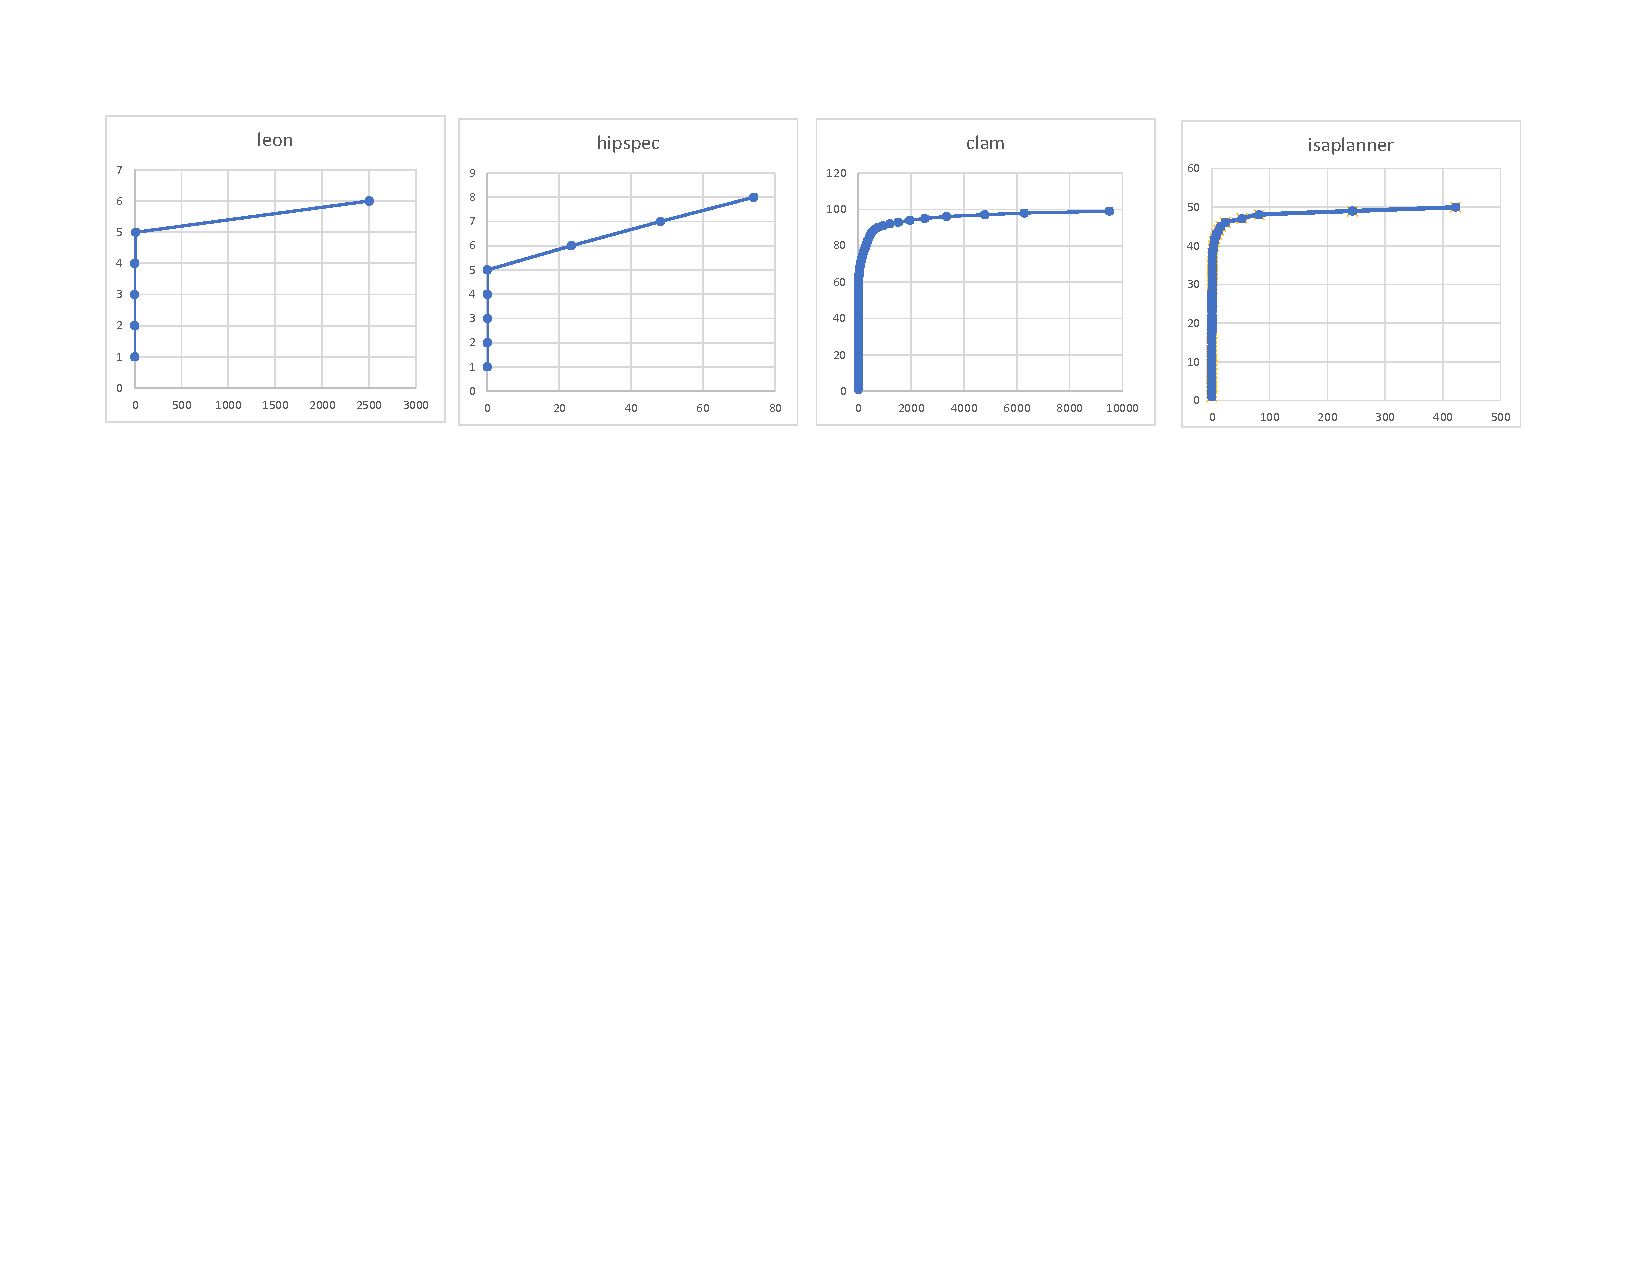
\includegraphics[width=\textwidth]{img/chart_solve_accum.pdf}
    %\newcommand\smaller{\fontsize{7pt}{7pt}\selectfont}

\begin{tikzpicture}
  \pgfplotsset{cactus/.style={
  		width=5cm,
        height=4cm,
        title style={yshift=-1pt,anchor=base},
        ytick distance=10^1,
        x tick label style={font={\smaller}},
        y tick label style={font=\tiny},
        ymajorgrids=true,
        %xlabel={benchmarks solved},
           mark size=.25pt}}

  \begin{axis}[title={clam}, cactus, ymode=log]
    \addplot[smooth,mark=*,green!50!gray] plot 
      table[y=time] {thesy/img/cvc4-benchmarks/cactus-clam.dat.txt};
  \end{axis}

  \begin{axis}[title={hipspec}, at={(5cm,0)}, cactus, ymode=log]
    \addplot[smooth,mark=*,green!50!gray] plot 
      table[y=time] {thesy/img/cvc4-benchmarks/cactus-hipspec.dat.txt};
  \end{axis}

  \begin{axis}[title={leon}, at={(0,-3.5cm)}, cactus, ymode=log]
    \addplot[smooth,mark=*,green!50!gray] plot 
      table[y=time] {thesy/img/cvc4-benchmarks/cactus-leon.dat.txt};
  \end{axis}

  \begin{axis}[title={isaplanner}, at={(5cm,-3.5cm)}, cactus, ymode=log]
    \addplot[smooth,mark=*,green!50!gray] plot 
      table[y=time] {thesy/img/cvc4-benchmarks/cactus-isaplanner.dat.txt};
  \end{axis}


\end{tikzpicture}

    \caption[Accumulated time-to-solve CVC4 benchmarks]{Accumulated time-to-solve for each of the benchmark suites from the CVC4 collection.
    The $y$ axis shows the amount of time needed to complete the first $x$ (successful) proofs, when benchmarks are sorted from shortest- to longest-running.}
    \label{results:solve-accum}
\end{figure}
\section{Related Work}
\label{thesy:related}

\begin{paragraph}{Equality Graphs}~
Originally brought into use for automated theorem proving~\cite{JACM2005:Detlefs},
e-graphs were popularized as a mechanism for implementing low-level compiler
optimizations~\cite{POPL2009:Tate}, under the name \emph{PEGs}.
These e-graphs can be used to represent a large
program space compactly by packing together equivalent programs.
In that sense they are similar to Version Space 
Algebras~\cite{ML2003:Programming}, but their prime objective is entirely
different.
While VSAs focus on efficient intersections, e-graphs are used to saturate a
space of expressions with all equality relations that can be inferred.
They have found use in optimizing expressions for more than just speed,
for example to increase numerical stability of floating-point programs
in Herbie~\cite{herbie}.
There are two key differences in the way e-graphs are used in this work compared
to prior:
(i) equality laws are not hard-coded nor fixed, they are fertilized
as the system proves more lemmas automatically;
(ii) saturation cannot be guaranteed or even obtained in all cases, which we overcome by a bound on rewrite-rule application depth.
(The latter point is an indirect consequence of the former.)
\end{paragraph}

\begin{paragraph}{Automated theorem provers}~
Many systems rely on known theorems or are designed to support users in semi-automated proving.
Congruence closure is also a proven method for tautology checking in
automated theorem provers, such as Vampire~\cite{vampire},
and is used as a decision procedure for reasoning about equality in leading SMT solvers
Z3~\cite{z3} and CVC4~\cite{cvc4}.
There, it is limited mostly to first-order reasoning, but can essentially
be applied unchanged to higher-level scenarios such as ours.

Related to theory exploration, but using separate techniques,
are Zipperposition~\cite{FroCoS2017:Cruanes}, and the conjecture generation mechanism implemented as part of
the induction prover in CVC4~\cite{cvc4induction}.
It should be noted, that these are directed toward a specific proof goal, as opposed to theory exploration, which is presumed to be an offline phase.
As such, the above two techniques incorporate generation of inductive hypotheses into the saturation proof search / SMT procedure, respectively.
\end{paragraph}

\begin{paragraph}{Theory exploration}~
IsaCoSy~\cite{JAR2010:Johansson} pioneered the use of synthesis techniques for bottom-up lemma discovery.
IsaCoSy combines equivalence reduction with coun\-ter\-ex\-ample-guided inductive synthesis 
(CEGIS~\cite{ASPLOS2006/Solar-Lezama}) for filtering candidate lemmas.
This requires a solver capable of generating counterexamples to equivalence.
Subsequent development was based on random generation of test values, as implemented in QuickSpec~%
\cite{JFP2017:Smallbone} for reasoning about Haskell programs, later combined with automated provers
for checking the generated conjectures~\cite{ICAD2013:Claessen,ITP2017:Johansson}.
We have mentioned the deficiencies of using concrete values (as opposed to symbolic ones) and random testing in \autoref{thesy:intro} and 
make an empirical comparison with Hipster, a descendent of IsaCoSy and QuickSpec, in \autoref{thesy:evaluation}.
%The need for automatic lemma discovery and proof is rising.
%First as helping users \cite{MathAid}, focus on probable lemmas, later on
%as automatic tools for building background knowledge for a domain %\cite{IsacoSy, Isascheme, hipspec, hipster}
%In his survey on Lemma discovery~\cite{ICICM2019:Johansson}, Johansson 
%/ HipSter and Into the Infinite for Haskell and Isabelle/HOL;
\end{paragraph}

\begin{paragraph}{Inductive synthesis}~
In the area of SyGuS~\cite{DSSE2015:Alur}, tractable bottom-up enumeration is commonly achieved
by some form of equivalence reduction~\cite{VMCAI2019:Smith}.
When dealing with concrete input-output examples, observational equivalence~%
\cite{CAV2103:Albarghouthi,Notices2013:Udupa} is very effective.
The use of symbolic examples in synthesis has been suggested~\cite{CAV2017:Drachsler}, but
to the best of our knowledge, ours is the only setting where symbolic observational equivalence
has been applied.
Inductive synthesis, in combination with abduction~\cite{STTT2017:Dillig},
has also been used to infer specifications~\cite{POPL2016:Albarghouthi},
although not as an exploration method but as a supporting mechanism for verification. 
\end{paragraph}

\begin{comment}
\begin{paragraph}{Rule-based knowledge}~
Software tools occasionally encode domain knowledge as a set of rewrite rules. 
The Haskell compiler GHC uses such rules when
performing optimizations such as Stream Fusion~\cite{SIGPLAN-Notices2007:Coutts}.
Term rewriting is also used in symbolic execution, to simplify the representation of symbolic states~\cite{FMCAD2008:Sinha}.
Typically, these rules are hand crafted.
This is a time-consuming and error-prone process, which catalyzes the interest of the programming languages community in automatic generation of them~\cite{arXiv2020:Murali}.
\end{paragraph}
\end{comment}

\section{Future Work}

\TheSy has been built from the grounds up based on term rewriting, and the results s what previous, non-symbolic tools have been able to accomplish.
However, it is our opinion that the advantages lie in its  potential to extend to new domains that cannot be
handled by concrete testing and SMT solvers.

Much of the appeal of \TheSy as a new technique for theory
exploration is its versatility in handling abstract values.
Since concrete data elements are not required for the lemma vetting process,
\TheSy can be extended to arbitrary families of types.
Our experiments have shown that it successfully handles first-class functions without generating the function bodies, but based solely on their signatures.
The next step would be to add support for refinement types~\cite{pldi91/freeman},
and notably, dependent types.
These were shown to be excellent tools in reasoning about the correctness of software~\cite{icfp14/vazou,book/cpdt,oopsla19/jad}.
In particular, their combination --- dependent refinement types --- is most interesting because it exposes the tight interconnection between types and propositions.
This makes it an ideal challenge for symbolic, constructive reasoning.

A second pain point, exposed by our experiments, is handling case splits when comparing terms as well as by carrying out proofs.
Testing technology has evolved several tools targeted specifically at handling conditional control flow in over 40 years of research in the field (\cite{cacm76/king}, with some commercial outcomes such as \cite{TaP2008:Tillman}).
The appeal of applying a proof-theoretic approach is its ability to employ mathematical abstractions to describe classes of values.
The current implementation of \TheSy essentially forks execution when splitting by case, copying the entire state.
A more careful treatment can distinguish facts that are case-specific from global ones, making the search more focused and allowing deeper proof exploration.
\chapter{Easter Egg: Equality Reasoning Based on E-Graphs with Multiple Assumptions}
\label{chap:colors}

\section{Introduction}
\label{colors:intro}

% Context
E-graphs are a versatile data structure that is used for various tasks of automated reasoning, including theorem proving and synthesis.
E-graphs have been popularized in compiler optimizations thanks to their ability to support efficient \emph{rewrites} over a large set of terms, while keeping a compact representation of all possible rewrite outcomes.
This mechanism is known as \emph{equality saturation}.
It provides a powerful engine that allows a reasoner to generate all equality consequences of a set of known, universally quantified, equalities.
Possible uses include selecting the best equivalent of an expression according to some desired metric, such as run-time efficiency~\cite{eqsat}, size~\cite{flatt2022small,DBLP:conf/fmcad/NotzliBNPRBT22}, or precision~\cite{herbie}
(when used as a compilation phase)
and a generalized form of unification, called e-unification, for application of inference steps (when used for proof search).

In this work we focus on a stepping stone for what we address as \emph{exploratory reasoning}: a range of tasks including all the above optimization procedures, as well as theory exploration \cite{thesy}, rewrite rule inference \cite{ruler}, and proof search \cite{vampire,DBLP:conf/aplas/BrotherstonGP12,cycleq}.
Exploratory reasoning, in general, can be thought of as any reasoning task navigating a large space of potential goals or sub-goals that need to be selected based on some criteria.
Our motivating example comes from TheSy and Ruler, both of which are theory exploration systems based on e-graphs. 
A theory exploration system attempts to both discover and prove mathematical properties from a set of definitions and known lemmas.
Most of the difficulty in theory exploration comes from the generation and filtering of candidates, rather then from the proof procedure itself.
TheSy does so by efficiently filtering a large set of potential conjectures using e-graphs for equality reasoning, and evaluating which should be potentially proved.
While e-graphs are effective for equality reasoning \cite{egg}, handling branching, such as case splitting during proof search, do not have a common solution, and are treated ad-hoc.
For example, a special type of node is introduced in \cite{eqsat} to deal with loop conditions, while in \cite{coward2023automating} a special operator is introduced to reason on expressions under certain contexts, and \cite{thesy} creates full copies of the e-graph for each branch being explored.

% Gap
To illustrate this difficulty, we zoom in on an example from theory exploration.
As an example scenario, consider trying to discover and prove lemmas on sorted lists:
a library containing functions $\tlfind$, $\tissorted$, and $\tbinsearch$.
We expect to discover lemmas involving these functions; one such lemma might be the property: $\tissorted\,l \rightarrow \tbinsearch\, l\,v = \tlfind\,l\,v$.
State-of-the-art theory exploration systems~\cite{ITP2017:Johansson,ruler,thesy} have some enumeration strategy over expressions in order to discover candidates. 
A challenge presents itself when some lemmas in the space require an assumption, in this case $\tissorted\,l$.
When dealing with e-graphs,
adding an assumption would \emph{globally}
affect all terms involved in the enumeration, making it impossible to separate conclusions stemming from different assumptions.
Because the system cannot know in advance which assumptions will become relevant for discovering equalities, it is required that it also generate and test multiple candidate assumptions.
An immediate solution is to create one copy of the graph per assumption, but doing so can significantly increase the memory usage.
Moreover, lemmas may depend on one another; for example, $\tissorted\,l \rightarrow \tbinsearch\, l\,v = \tlfind\,l\,v$ depends on transitivity of $\leq$ ($x\leq y \land y\leq z \rightarrow x\leq z$).
Therefore, just trying the candidates one at a time would mean that the system would prematurely discard candidates depending on the order in which they are tested; alternatively, for each candidate that is validated and becomes a lemma, it would be forced to re-try all the previously failed attempts, which is highly costly.

% Theory exploration systems based on random testing  (\todo{speculate, hipspec with conditions}) attempt to greedily discover

% Innovation
To overcome this difficulty, we propose an extension of the e-graph data structure.
An e-graph naturally represents a congruence relation $\cong$, which is an equivalence relation over terms (with function applications), which  maintains $x \cong y \vdash f(x) \cong f(y)$ (see \autoref{perlims:congrel}).
The congruence relation is maintained in the e-graph as a set of equivalence classes (e-classes), which can be merged as part of updating the underlying relation. 
We extend the e-graph data structure into a \emph{Colored E-Graph} to maintain multiple congruence relations at once, where each relation is associated with a color.
Our key observation is that each added assumption, can be treated as a new congruence relation, but is only a coarsening of the original relation. 
The coarsening, then, can be represented as a set of additional merges of e-classes on top of the original e-graph.
The main benefit is reducing memory consumption by re-using and sharing most of the e-classes between colors.
Going back to the sorted list example, in the colored e-graph there will be a \cred relation for assuming $x \le y \land y \le z$, and a \cblue relation for assuming $\tissorted\,l$.
Thanks to the size reduction, multiple relations can exist at once, and thus the lemma $\tissorted\,l \rightarrow \tbinsearch\, l\,v = \tlfind\,l\,v$ can be discovered after transitivity of $\leq$ is proven, but without dependency on the order of exploration.
Colored e-graphs also support having a hierarchy between different colors, which can benefit from additional sharing of e-classes.
For example, the \cred color representing $x \le y \land y \le z$ is itself a coarsening of some \cgreen color representing just the assumption $x \le y$.

While the memory footprint for each color is smaller, maintaining the congruence relation and the data structure invariants becomes more challenging.
To address this we present specialized data-structure modifications and evaluate them.
%We also extend the colored e-graph's logic in several key ways, to support e-graph operations for all the colors.
First, we set up a multi-level union-find where the lowest level corresponds to the root congruence.
Second, we change how congruence closure is applied to the individual congruence relations while taking advantage of the sharing between each such relation and the root. 
Lastly, we present a technique for efficient e-matching over all the relations at once.

% Oh we are so good!
\medskip
Our contributions are:
\begin{enumerate}[leftmargin=1.1em]
    \item The observation that assumptions induce coarsened e-graphs that share much of the original structure. 
    \item Algorithms for colored e-graphs operations.
    \item Optimizations on top of the basic algorithms to significantly improve resource usage.
    \item A colored e-graph implementation, \emph{Easter Egg}\footnote{\url{https://github.com/eytans/egg/tree/features/color_splits}} and an evaluation that shows an improvement factor in memory usage over the existing baseline, while maintaining similar run-time performance.
\end{enumerate}
\section{Overview}
\label{chap:colored-egraph}
\label{colors:overview}

% <The story goes:>
% 1. Connect motivation (from intro) to egg (as described in background), highlight uses in TheSy (and ruler)
% 2. General concept of colored (layered) e-classes
%    2.a. Explain clone semantics and how colored e-classes are equivalent
% 3. What e-graph operations need to be modified to support colored e-classes
% 4. Challenges and problems (performance bottlenecks caused by the new design)
% 5. Summary of optimization (primer for next section)

\begin{figure}[t]
  \centering
\begin{comment}
  \node(black)[label={above:$\cong$},
               label={[sub]below:{\small (a)}}] {
  %$\cong$ & $\congblue$ & $\congred$ \\
    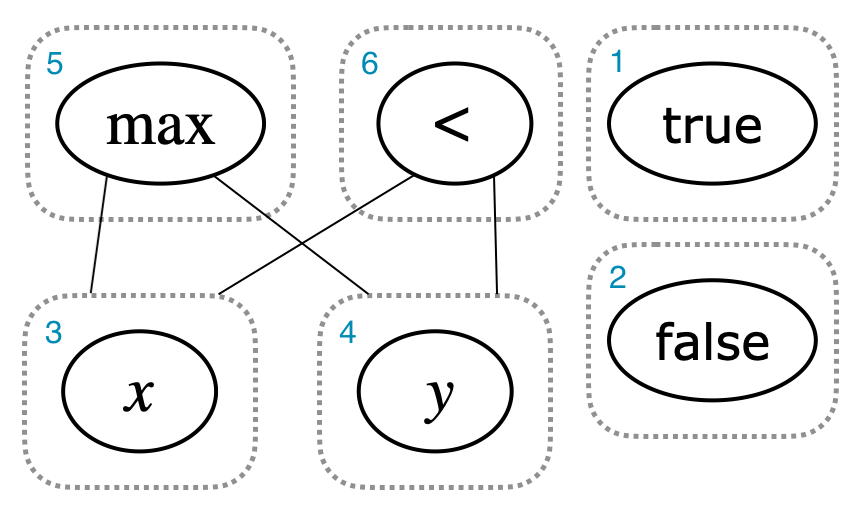
\includegraphics[width=2.7cm,valign=c]{gfx/egraph-max.png}
  };
\end{comment}

  \begin{tikzpicture}[sub/.style={label distance=0,outer sep=0,inner sep=0}]
  \node(blue) [label={[sub]above:$\congblue\!\!$},
               label={[sub]below:{\small (a)}}] {
    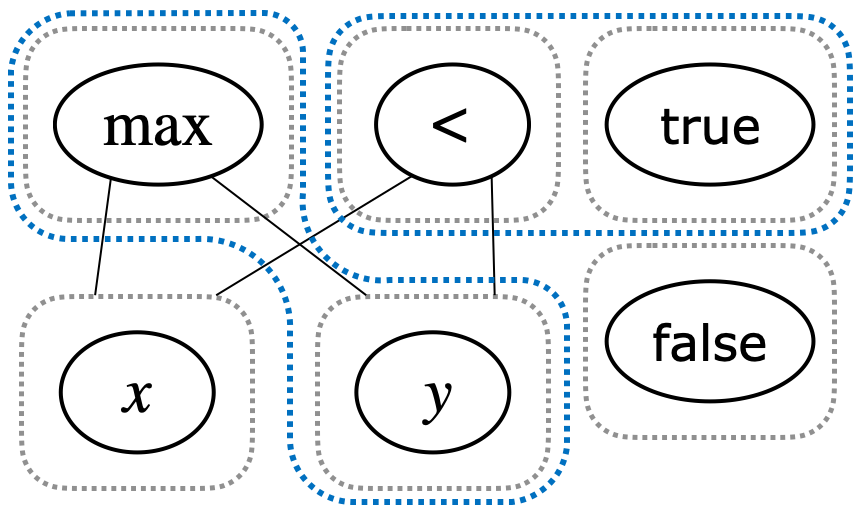
\includegraphics[width=2.7cm,valign=c]{colors/gfx/egraph-max-blue.png}    
  };
  \node(red)[right=0mm of blue,
             label={[sub]above:$\congred$},
             label={[sub]below:{\small (b)}}] {
    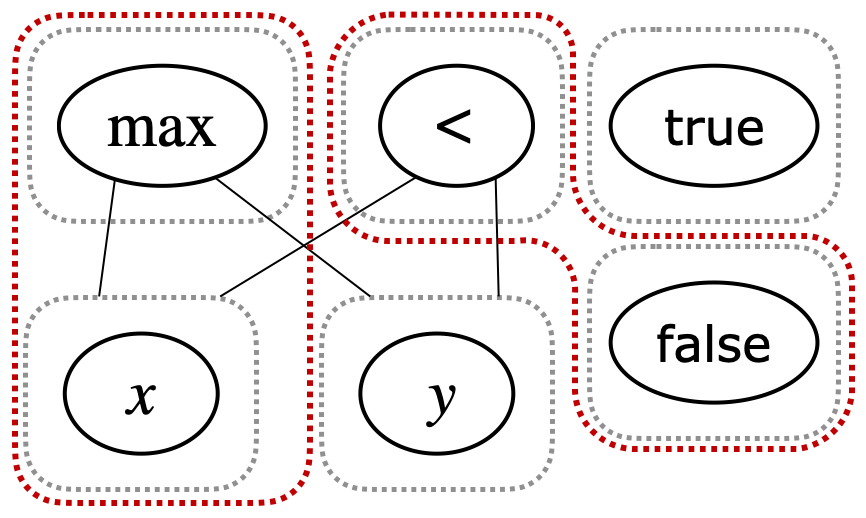
\includegraphics[width=2.7cm,valign=c]{colors/gfx/egraph-max-red.png}
  };
  \node(mixed)[right=0mm of red,
               label={[sub]below:{\small (c)}}] {
    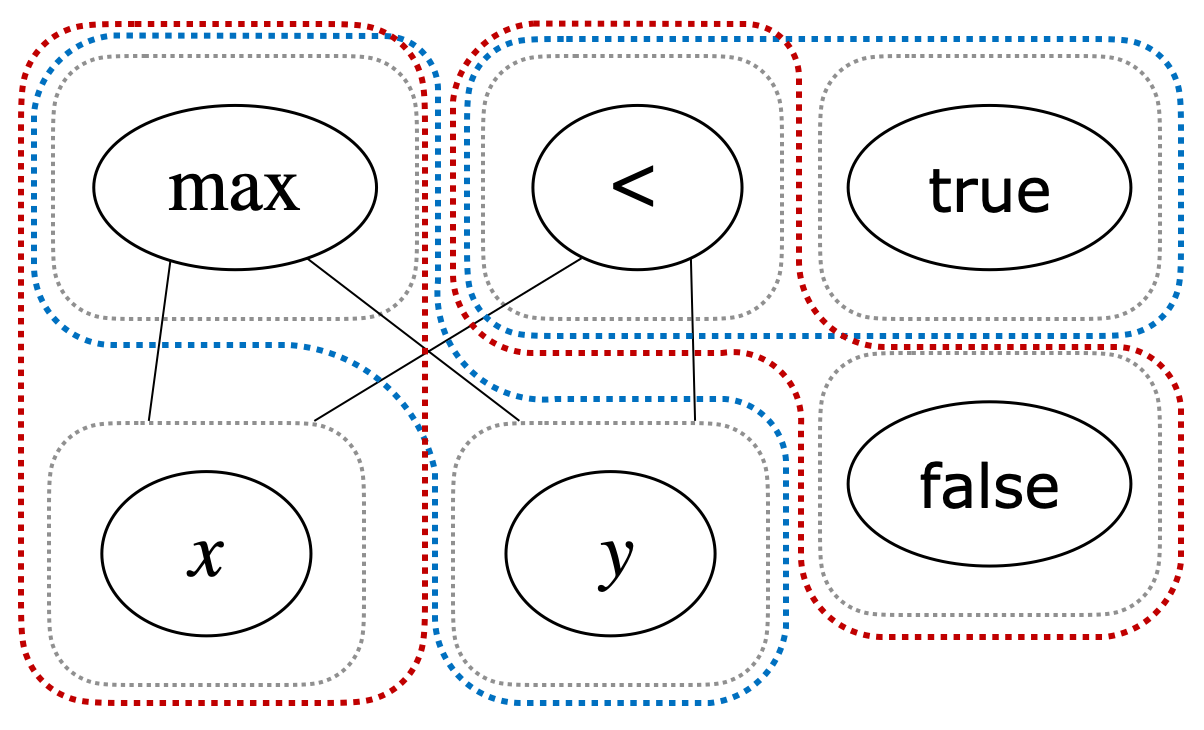
\includegraphics[width=2.9cm]{colors/gfx/egraph-max-red-blue.png}  
  };
  \end{tikzpicture}
  \vspace{-1.5em}
  \caption{Example e-graph with two colored layers; (a) is blue, (b) is red, (c) shows them combined.}
  \label{overview:egraph-max}
\end{figure}

From this point we assume familiarity with the basic e-graph structure which includes a union-find, hashcons, and an e-class map, as well as the basic operations of add, merge, rebuild, and e-matching (and consequently rewriting).
For readers unfamiliar with e-graphs, or with deferred rebuilding, which was introduced in \cite{egg}, additional background is given in  \annexref{background}. \ES{todo put in some real background}

\emph{Colored E-graphs} are an extension of e-graphs devised to add a generic approach for supporting conditional reasoning to e-graphs.
Existing exploratory reasoning systems such as TheSy~\cite{thesy} and Ruler~\cite{ruler} utilize equality saturation with e-graphs for discovering new rewrite rules, but are limited in the presence of conditionals.
For example, let $t := \tmax(x, y)$, then reasoning about the cases $x < y$ and $x \geq y$ separately is desirable: in the first case $t \cong x$, and in the second $t \cong y$.
Without any assumptions, we can say neither and rewriting of $t$ is blocked.
The approach in \cite{thesy} involves a prover that creates an e-graph \emph{clone} for each case in case splitting, such as for $x < y$ and $x \geq y$. 
This process, however, incurs high runtime and memory costs. 
Non-relevant terms in the e-graph are unnecessarily duplicated, and rewrites are redundantly applied to these copies. 
Further case splits compound this issue, leading to an exponential increase in the number of clones with additional nested splits.

%\ES{represent colored e-graphs shortly because it was last seen in the intro}

Colored e-graphs are designed to avoid duplication via sharing of the common terms, thus storing them only once when possible.
The e-graph structure becomes \emph{layered}:
the lowermost layer represents a congruence relation over terms that is true in all cases (represented, normally, as e-classes containing e-nodes).
On top of it are layered additional congruence relations that arise from various assumptions.


Going back to our example, the corresponding e-graph is
shown in \autoref{overview:egraph-max},
containing the terms $\tmax(x, y)$, $x < y$, $\ttrue$ and $\tfalse$.
Layers corresponding to assumptions $x < y$ and $x \geq y$ are shown in \ref{overview:egraph-max}(a) and \ref{overview:egraph-max}(b).
To evoke intuition, we associate with each layer a unique \emph{color}, and paint their e-classes (dotted outlines, in depicted e-graphs) accordingly.
Conventionally, the lowermost layer is associated with the color black.
In the subsequent example we will use \cblue for $x<y$ and \cred for $x\geq y$ when referring to the example.
In the \cblue layer, $(x < y) \congblue \ttrue$ and
$\tmax(x, y) \congblue y$;
in the \cred layer, $(x < y) \congred \tfalse$
and $\tmax(x, y) \congred x$.
This is shown via the corresponding 
\cblue and \cred dotted borders.
\autoref{overview:egraph-max}(c) shows a depiction where both colors are overlain on the same graph, which is a more faithful representation of the concept of colored e-graphs,
although this visualization is clearly not scalable to larger graphs.
In \autoref{overview:egraph-max-min}, a larger graph can be seen that includes the terms $\tmax(x,y)-\tmin(x,y)$ and $|x-y|$.
An overlain graph will be quite incomprehensible in this case, so the layers are shown separately; it can be easily discerned that $\tmax(x,y)-\tmin(x,y) \congblue |x-y|$
as well as $\tmax(x,y)-\tmin(x,y) \congred |x-y|$.

\begin{figure*}[t]
  \centering
  \begin{tabular}{@{}ccc@{}}
    $\cong$ & $\congblue$ & $\congred$ \\
    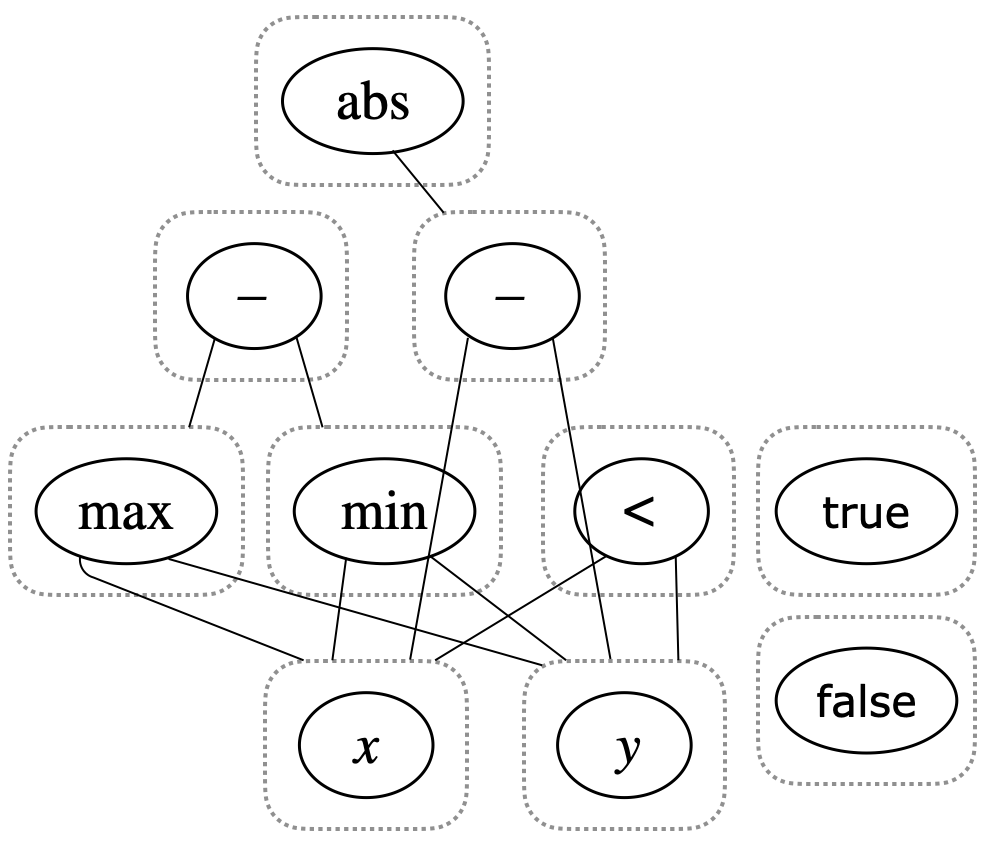
\includegraphics[width=0.25\textwidth]{colors/gfx/egraph-max-min.png} &
    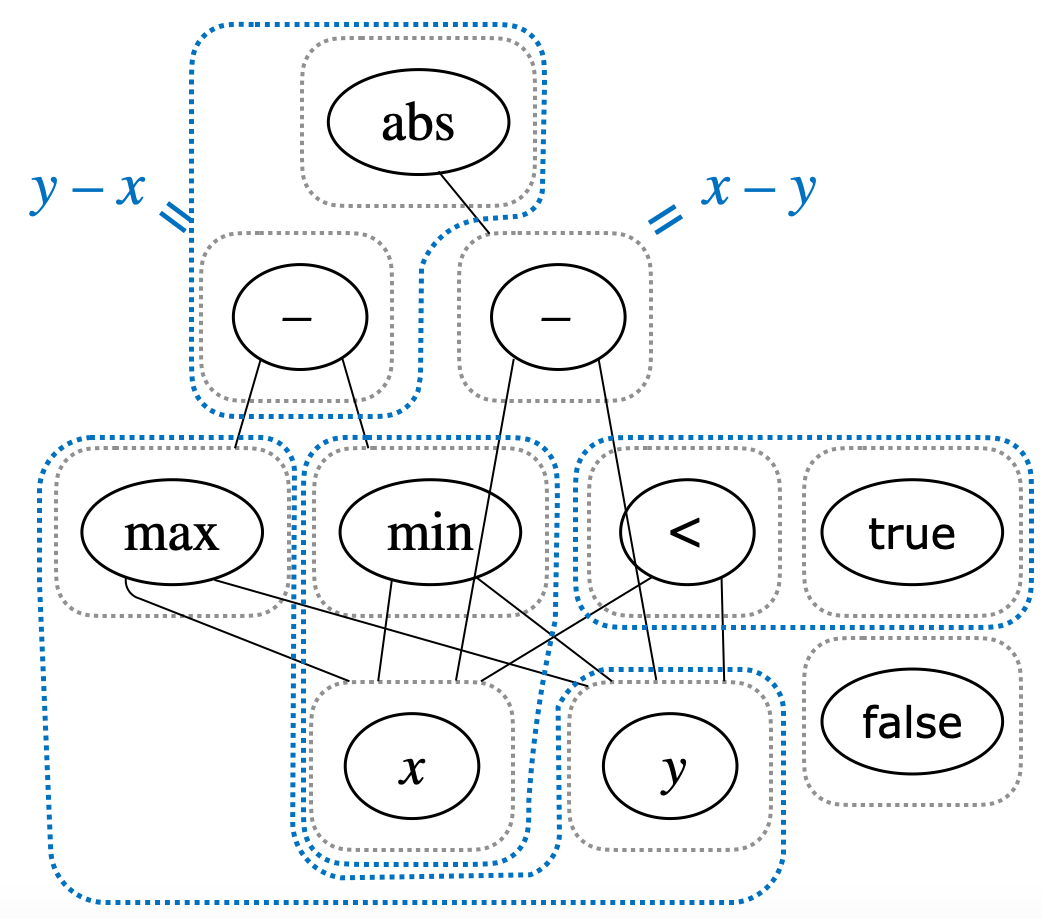
\includegraphics[width=0.25\textwidth]{colors/gfx/egraph-max-min-blue.png} &
    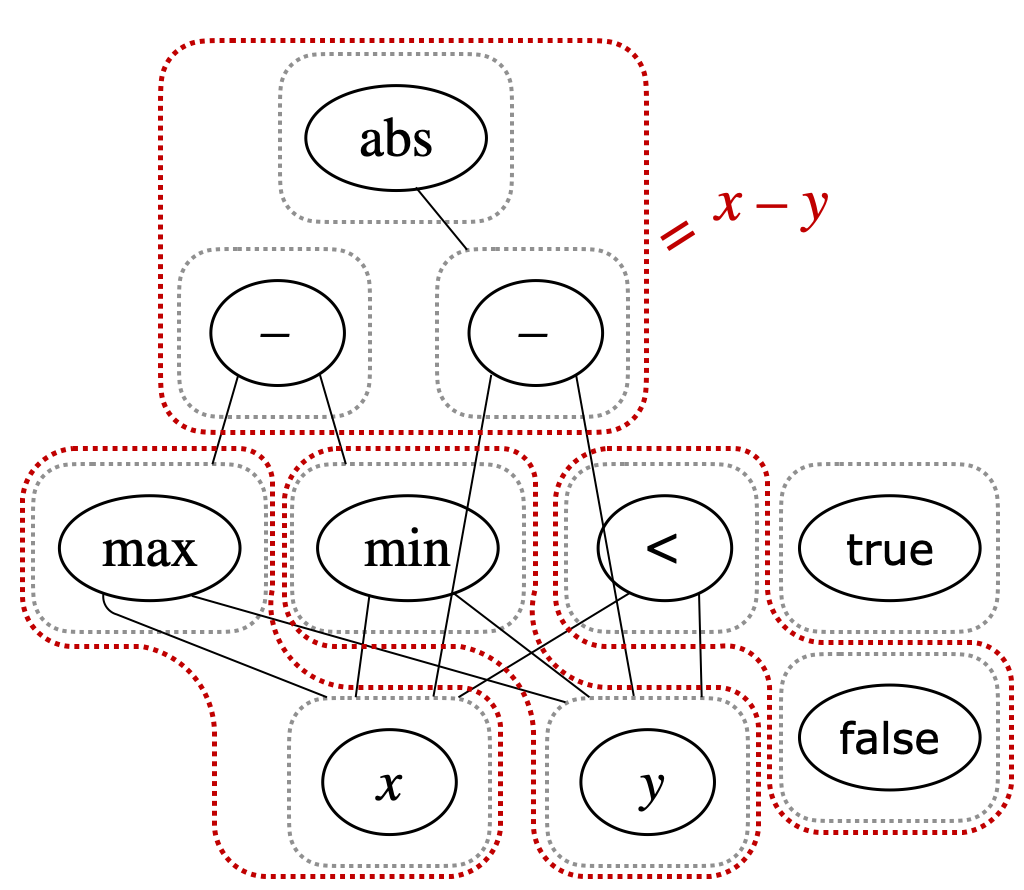
\includegraphics[width=0.25\textwidth]{colors/gfx/egraph-max-min-red.png}
    \\
    {\small (a)} & {\small (b)} & {\small (c)}
  \end{tabular}
  \caption{Proof of $\tsmallmax(x,y)-\tsmallmin(x,y)=|x-y|$.
  The e-nodes corresponding to the two terms are in the same e-class both in the blue layer (b) and in the red (c).
   It is important to note that the layers are overlain, and that the black nodes are shared; they are separated here for ease of perception.}
  \label{overview:egraph-max-min}
\end{figure*}

Both additional layers, \cblue and \cred, use existing (black) e-nodes, with each color represented by further unions of e-classes in the black congruence relation. 
Each color's congruence $\cong_c$ is a \emph{coarsening} of the black congruence, $\cong$, as ${\cong}\subseteq{\cong_c}$.
% Hierarchy exmaple
In complex cases like the generalization of $\tmax(x,y)-\tmin(x,y) \cong |x-y|$ to $\tmax(x,y,z)-\tmin(x,y,z) \cong \tmax(|x-y|, |x-z|, |y-z|)$, the colored e-graphs have an important layered structure. 
This scenario requires reasoning about additional assumptions, building additional layers, such as $x < y \land y < z$ on top of $x < y$ (and respectively $x \ge y \land y < z$ on top of $x \ge y$). 
These additional layers will reuse the \cblue and \cred ones, as they are a coarsening of the respective $\congblue$ and $\congred$.

\begin{comment}
The extra colors are due to the conditionals from $\tmax$, $\tmin$, and $|\,{\cdot}\,|$ leading to a total of six leaf cases as can be seen in \autoref{overview:minmax-splits}.
The coarsening of congruence relation holds in this multi-level hierarchy as well.
If we mark in \cblue the layer representing $(x < y) \congblue \ttrue$, and in \cgreen the layer representing $x < y \land y < z \conggreen \ttrue$, then ${\congblue}\subseteq{\conggreen}$.
That is, any common sub-term and conclusion made in root, or one of the parent colors can be shared to the descendants.
Thus, further duplication, whether of terms or computation, can be prevented.
%Note, that this is not a full tree as in some cases we can conclude the $<$ relation between $x$ and $z$. 
%For example, in the case of $x < y \land y < z$ we can conclude $x < z$ without additional case splitting.

\begin{figure}
\begin{tikzpicture}[
    grow=down,
    level 1/.style={sibling distance=50mm, level distance=20mm},
    level 2/.style={sibling distance=25mm, level distance=20mm},
    level 3/.style={sibling distance=25mm, level distance=20mm},
    edge from parent/.style={->, draw},
    >=latex,
    every node/.style={align=center}]

% root of the tree
\node (root) {root}
% children of root
    child{node {$x < y$}
        % children of "x >= y"
        child{node {$x < y \land y \ge z$}
            child{node {$\cdots \land x < z$}}
            child{node {$\cdots \land x \ge z$}}
        }
        child{node {$x < y \land y < z$}}
    }
    child{node {$x \ge y$}
        % children of "x < y"
        child{node {$x \ge y \land y \ge z$}}
        child{node {$x \ge y \land y < z$}
            child{node {$\cdots \land x < z$}}
            child{node {$\cdots \land x \ge z$}}
        }
    };
\end{tikzpicture}
\caption{All needed case split cases to reason about the property $\tmax(x,y,z)-\tmin(x,y,z) \cong \tmax(|x-y|, |x-z|, |y-z|)$}
\label{overview:minmax-splits}
\end{figure}
\end{comment}

\begin{comment}
A crucial challenge to address is the implementation of operations (insert, union, congruence closure, e-matching)
efficiently while preserving this invariant as well as the standard e-graph invariants.
The colored layers require special support, as different e-classes may be united in some colored (non-black) layer but not in others (including the black relation). 
Notably, the black congruence relation can be implemented as a standard e-graph since all the necessary data structures are available to it.
\end{comment}

% Clone semantics
Before diving into the design of colored e-graphs, it is better to start with their expected semantics.
One way to understand the semantics of colored e-graphs is by analogy to a set of clones, i.e. separate e-graphs $\mathcal{E}$.
One e-graph represents the base congruence $\cong$,
and one e-graph per color $c$ represents $\cong_c$.
All e-graphs in $\mathcal{E}$ conceptually represent the same terms partitioned differently into e-classes.
Thus, they have the same e-nodes, except that the choice of e-class id (the representative) may be different according to the composition of the e-classes.
We will call the e-classes of the color congruences \emph{colored e-classes}.
A union in any layer, black or colored, is in effect a union applied to the respective e-graph and all its descendants. 
Thus, a union in the black layer (i.e. the original e-graph) is analogous to a union in \emph{all} of the e-graphs of the corresponding e-classes;
this maintains the invariant that every colored e-class is a union of (one or more) black e-classes.
The colored e-graph semantics of the other operations---insertion, congruence closure, and e-matching---are the same as if they were performed across all clones.

\begin{comment}
Using a set of e-graphs is very similar to what TheSy does.
But, this set of e-graphs approach proves to be inefficient in exploratory reasoning tasks. 
The main issue is that with each e-graph consisting of its own hash-cons, union-find, and e-class map, the memory consumption will be significant.
However, in some cases a separate e-graph could be quite efficient.
An extreme (but not uncommon) case is when an e-graph becomes inconsistent, which can be when \eg $\ttrue$ is union-ed with $\tfalse$.
This can lead to many e-classes representing Boolean expressions being union-ed, and as a side effect, requiring much fewer e-nodes.
For example $\ttrue \land \ttrue$, $\ttrue \land \tfalse$, $\tfalse \land \ttrue$, and $\tfalse \land \tfalse$ will all be represented by the same e-node $[\ttrue] \land [\ttrue]$.
In this case, when the e-graph rebuilds it will minimize itself.
The e-graph memory footprint could actually be as small as the size of the union-find plus a constant amount of e-nodes.\SI{I am a bit unsure about how `constant' this amount is; still sounds polynomial in the number of e-classes}
\end{comment}

A guiding observation in the design is that in equality saturation based exploratory reasoning tasks, where the e-graphs are extensive, each assumption leads to modest increase in congruences.
Colored e-graphs are adapted to this scenario.
The basic presupposition is that most colored layers, like the \cblue layer in \autoref{overview:egraph-max-min}, do not involve an excessive amount of additional unions.
In these cases, the space savings from not duplicating black e-nodes more than compensate for the added complexity in managing colored e-classes. 
With careful tweaks and a few optimizations, we show that we improve upon a clone-based approach.
Importantly, if the assumption leads to an inordinate increase in additional unions, the clone-based approach could be more appropriate, and it is possible to use a clone for that specific assumption.

%\SI{there is some commented-out content here}
\begin{comment}
%As we will show later, the colored e-graph performs worse when many changes are done on top of the original e-graph \ES{TODO: show and link?}.
And so, colored e-graphs and separate e-graphs are approaches that complement each other.
An obvious optimization is to automatically switch from a colored layer into a new separate e-graph on the fly.
This can potentially improve performance, but automatically detecting when it is useful, and then switching is something we leave for future work. 
\ES{TODO: we need to make sure we right about the inherent problems in the colored e-graph implementation when there are many changes (after the optimizations). then add this but with more detail: Although it might seems like a limitation, but actually we can always decide to drop a color, or explore it in a new separate E-Graph.}
\end{comment}

% The most basic setup. Without colored e-nodes, only how we implement rebuild and e-mathcing.
For presentation purposes, we start with a basic implementation that is not very efficient but is effective for understanding the concepts and data structures;
then, we indicate some pain points, and move on to describe optimization steps that can alleviate them.

In the basic implementation, all e-nodes reside in the ``black'' layer,  represented by a ``vanilla'' e-graph implemented in egg, with normal operations.
The colored congruences do not have designated e-graphs of their own, and instead, the operations of merge, rebuild, and e-matching have \emph{colored variants}, parameterized by an additional color $c$, that are semantically analogous to the same operations having been applied, in clone semantics, to the e-graph associated with color $c$ in $\mathcal{E}$.
(Insertion is deferred to later.)
%(For the time being, insertion does not have a colored variant, since insertions create e-nodes and all e-nodes are shared.)

\myparagraph{Colored merge.}
In colored e-graphs, the union-find structure used for merging, which traditionally holds all e-class ids, is optimized. 
A master copy retains black unions, while each color layer has a \emph{smaller} union-find for merged representative e-classes of the parent layer. 
This approach avoids replication of data across layers.

\myparagraph{Colored e-matching.}
The e-class map is only saved for the black layer.
This is sufficient, because an e-class in color $c$ is always going to be a union of black e-classes, and all that is required for e-matching is finding e-nodes with a particular root (operator) in the course of the top-down traversal.
So the union can be searched on demand by collecting all the ``$c$-color siblings'' of the e-class and searching them as well.

\myparagraph{Colored congruence closure.}
In egg, the e-graph maintains congruence by cycling through a work list of altered classes, re-canonizing their parents, and identifying unions to complete congruence through duplicate detection.
In colored e-graphs the root will behave the same, but for colored layers there is no single e-class, as the colored e-classes are a equality class of concrete e-classes.
For each color, we maintain an additional work list and collect concrete parents from e-classes on demand. 
This results in a rebuild algorithm similar to egg's, but without updating the hashcons in colored layers, as they are not present.

For a more concrete example, we give a detailed walkthrough of equality saturation in a colored e-graph of the \cred case from  \autoref{overview:egraph-max-min}(b), and show the steps taken
to construct this colored layer in \annexref{app-b}.

When using the above operations in the context of equality saturation, e-matching is applied for all colors
% \SI{should we describe the machine way to do it in a combined pass or leave it for optimizations} - Leave for optimizations. It is a non trivial optimization to say black matches cover colored ones. 
to discover matches for the left-hand sides of rules.
For each match, the right-hand side of the rule needs to be inserted into the e-graph and merged or color-merged with the left-hand side.
Inserting the e-nodes to the e-graphs makes them available to all layers.
This aspect is sound, since
we assume that the mere \emph{existence} of a term in an e-graph does not in itself have the semantics of a judgement---it is only the placing e-nodes in the same e-class that asserts an equality.
However, in the presence of many colors, and thus many colored matches, the result would be a large volume of e-nodes that are in black e-classes of size 1, as they
were created to serve a single color.
As opposed to a, standard, single e-graph where merging e-classes shrinks the space of e-nodes (because non-equal e-nodes may become equal as a result of canonization),
in colored unions it is required that the e-graph maintain both original e-classes, thus losing this advantage.
This can put a growing pressure on subsequent e-matching and rebuild operations \emph{in all colors}.
Optimizations to improve colored e-graphs, and to address this issue, are presented in \autoref{colors:optimizations}.


\begin{comment}
   {\color{gray} 
\noindent\textbf{Colored insert.}~
As discussed, e-nodes should be shared, but until now no new e-nodes were added.
A simple example is the e-graph for the terms $1 + 2$, $2 + 1$ and $x$.
Now consider a new {\color{blue}blue} relation, and have the blue union $1 \congblue x$.
When we apply addition commutativity on this e-graph, a new e-node, ($1~+~x \rightarrow x~+~1$), should be added, but only for the blue layer.
In the current unoptimized approach, we share all e-nodes, so there will only be black e-nodes.
Meaning we will add the e-node to the original e-graph, but only unify the e-classes in the blue layer.
\ES{Should this be a theorem?} It is sound under the assumption that any e-node in the e-graph does not have any semantic meaning by itself.
For example, when encoding a problem to the colored e-graph, $sorted(l)$ has no semantic meaning unless $sorted(l) \cong true$ or $sorted(l) \cong false$.
And, If an additional e-node represented in the original e-graph does not affect the semantics, it is safe to add all colored conclusions as black e-nodes.


% Caveats and intro to optimizations section
To understand the weakness of this simple approach we should consider the setting of equality saturation.
A color will have additional unions, and therefore, might apply more rewrites resulting in additional e-nodes. 
The most basic approach of adding these e-nodes to the existing e-classes, hash-cons, and parents, is sound, but will result in additional e-matching results.
When considering the example from before, all colors can match on $x~+~1$.
A larger e-graph with more e-matches will lead to more rewrite rules being applied, and a slower rebuild process.
In addition, colored e-matching can find colored un-canonized matches.
Canonizing matches using the black congruence relation may lead to the addition of many unneeded e-nodes, as colored e-matching might produce duplicate matches.
But, canonizing using the colored congruence relation might produce different e-nodes for each color.
What makes matters more difficult, is that when all e-nodes are part of the original e-graph, they will not remain canonized by the colored relation, and might become "dangling" \ES{We will need to work on these explanations}.
}
\end{comment}

\section{Functional Description}
\label{colors:functional}

We now introduce some notations and definitions that formalize
the description of the e-graph presented in \autoref{colors:overview}.
We assume a term language $L$ where terms are constructed using \emph{function symbols}, each with its designated arity.
We use $f^{(r)}\in\Sigma[L]$ to say that $f$ is
in the \emph{signature} of $L$ and has arity $r$.
A term is then a \emph{tree} whose nodes are labeled by function symbols and a node labeled by $f$ has $r$ children.
(In particular, the leaves of a term have nullary function symbols.)
Additionally we use the following definitions:
%
\[
\renewcommand\arraystretch{1.2}
\begin{array}{ll}
  \mbox{e-class ids} & E  \\
  \mbox{e-nodes}  & N = \{f(e_1,..,e_r)~|~ f^r\in\Sigma, e_i\in E\} \\
  \mbox{union-find} & {\eqid} \subseteq E\times E, \quad \mbox{${\eqid}$ is an equivalence relation} \\
  \mbox{e-class map} & M : E \to \mathcal{P}(N) \\
  \mbox{parent map}  & P = \{e \mapsto \{ (n, e') ~|~ e' \in E~\land \\
  & \quad n \in M(e') \land n = f(\ldots, e, \ldots) \} ~|~ e \in E \} \\
  \mbox{hashcons} & H = \{n\mapsto e ~|~ n\in M(e)\} \\
\end{array}
\]

Semantically, every e-class represents a set of terms over $\Sigma$.
We will use the notation $[t]$ to refer to e-class id of the equality class that represents (among other terms), the term $t$.

The union-find structure offers an operation, $\tfind(e)$, that returns a unique representative id of the equivalence class (of $\eqid$) that contains $e$.
That is, $\tfind(e) \eqid e$ and for all $e_1 \eqid e_2$, $\tfind(e_1) = \tfind(e_2)$.

On top of these basic structures, we introduce a set of \emph{colors}. 
As explained in \autoref{colors:overview}, colors are organized in a tree whose root is the initial color (``black'').
We mark the root color $\croot$
and assign to every non-root color $c$ a \emph{parent color} $p(c)$.
%
\begin{comment}
\[
\begin{array}{ll@{~~~}l}
\mbox{color tree} & C = \{\croot, \ldots\}
& p : C \setminus \{\croot\} \to C
\end{array}
\]
\end{comment}
\[
\renewcommand\arraystretch{1.2}
\begin{array}{ll}
  \mbox{colors} & C = \{\croot, \ldots\}  \\
  \mbox{parent colors} & p : C \setminus \{\croot\} \to C
\end{array}\hspace{2cm}
\]

\smallskip
The colored e-graph will now hold multiple union-find structures, one per color.
They define a family of equivalence relations $\equiv_{c}$ by induction
on the path from $\croot$ to $c$.

\begin{itemize}
    \item ${\equiv_{\varnothing}} = {\eqid}$~;\quad $\tfind_{\varnothing}(e) = \tfind(e)$
    \item ${\equiv_c} \subseteq E_{p(c)}\times E_{p(c)}$, where
      $E_{p(c)}=\{\tfind_{p(c)}(e)~|~e\in E\}$ is the set of all representatives from $\equiv_{p(c)}$. $\tfind_c\hspace{-0.5pt}(e)$ for $e\in E_{p(c)}$ returns a unique identifier in the normal manner of union-find, \ie, $\tfind_c\hspace{-0.5pt}(e) \equiv_c e$  and for all $e_1 \equiv_c e_2$, $\tfind_c\hspace{-0.5pt}(e_1) = \tfind_c\hspace{-0.5pt}(e_2)$.
\end{itemize}


\begin{comment}
Formalize the colored-rebuild algorithm
This should include an algorithmic description of normal rebuild
Then we would use functions to use the same algorithm for colored rebuild.
The main concerns that change are:
1. Collecting all the parents
2. Updating the memo
\end{comment}

The definitions over $E_{p(c)}$ are naturally extended to $E$ by (recursive) application of $\tfind$; i.e., $\tfind_c(e) = \tfind_c(\tfind_{p(c)}(e))$
and $e_1 \equiv_c e_2 \Leftrightarrow \tfind_{p(c)}(e_1) \equiv_c \tfind_{p(c)}(e_2)$.
Thus it holds, by construction, that
${\equiv_{c}} \supseteq {\equiv_{p(c)}}$.

The colored e-graph also supports a $\tmerge_c(e_1, e_2)$ operation for each color $c$ where $e_1, e_2 \in E_c$.
The merge operation may break the congruence relation invariants for $c$ and all its descendants, and thus needs to be fixed.
The merged classes are added to $\mathit{worklist}(c')$ for all $c'$ where $c'$ is $c$ or one of its descendant.
In egg~\cite{egg}, the invariants are restored periodically by performing a \textsc{rebuild} pass.
To accommodate the colors, we adjust the
\textsc{rebuild} logic to a multi-congruence-relation setting,
so that it restores a congruence closure for each color during \textsc{rebuild}.
The main difference is that for a colored congruence relation, the procedure will collect the parents of a colored e-class by combining the sets of parents of all the (root) e-classes contained therein.

\begin{comment}
We update the auxiliary function \textsc{repair}
to work on colored e-classes,
and introduce two new helper functions: $\textsc{collect\_parents}$ and $\textsc{update\_hashcons}$, as presented in \autoref{functional:repair}.
$\textsc{collect\_parents}$ extract the parents of a colored e-class by combining the sets of parents of all the (root) e-classes contained therein.
$\textsc{update\_hashcons}$ is used to make sure that the hashcons entries are in canonical forms. It was already a part of \textsc{repair} in egg;
it is only repeated here to point out that it
only updates the hashcons for the root color,
since no canonization is required for colored layers.    
\end{comment}

Another important colored e-graph operation is e-matching.
Colored e-matching is a modification of the e-matching abstract machine presented in \cite{DBLP:conf/cade/MouraB07}.
E-matching is performed by an abstract machine $M$ which consists of a program counter, array of registers $reg$, and backtracking stack $bs$, in combination with a sequence of instructions that represents a pattern $p$. 
The machine will run instructions by order, where each may either fail if its assertion is not met, or produce a set of continuation states.
If a continuation state is produced, the machine selects the first one and adds the current instruction to the stack. 
If no continuation state is produced, the machine backtracks, retrieving the most recent state from the stack and attempting the next available continuation.

To better present our modifications in colored egg, we first shortly introduce some of the original instruction types:
\begin{itemize}[leftmargin=1.1em]
    %\item $\iinit(f)$ --- Expects an e-node representing an application $f(x_1,\ldots,x_n)$ in $\treg[0]$, and pushes its children into $reg[1..n]$.
    \item $\ibind(\tin, f, \tout)$ --- Matches any e-node of the form $f(x_1,\ldots,x_n)$ that resides in the e-class saved in $reg[in]$, storing its children $x_{1..n}$ in $reg[out..out+n-1]$.
    \item $\icompare(i, j)$ --- Asserts $\treg[i] == \treg[j]$.
    \item $\icheck(i, term)$ --- Asserts that the e-class $\treg[i]$ represents $\tterm$.
    \item $\icontinue(f, out)$ --- Match any e-node 
    $f(x_1,\ldots,x_n)$ (in \emph{any} e-class),
    storing its children $x_{1..n}$ in $\treg[\tout..\tout+n-1]$.
    \item $\ijoin(\tin, \trevpath, \tout)$ --- Match any e-node
    $f(x_1,\ldots,x_n)$ that is reachable through $\trevpath$
    from the e-class $\treg[\tin]$,
    storing its children $x_{1..n}$ in $\treg[\tout..\tout+n-1]$.
\end{itemize}

To facilitate matching across various congruence relations, we adjust the machine $M$ to include the, currently being e-matched, colored assumption $color$ in its state.
Adapting to $color$ involves changes in compilation and instructions. 
The two primary scenarios impacted are: during $\icompare(i, j)$, ensuring $\treg[i] \equiv_{color} \treg[j]$, and in function application matching represented by a \ibind~ instruction.
Before each `\ibind' instruction, the modified compilation will insert a new `\iclrjmp' instruction to try matching the full colored equality class, one ``root'' e-class at a time.
This is achieved by having `$\iclrjmp(i)$' yield all the ``colored siblings'' of $\treg[i]$ in the current $\tcolor$, replacing $\treg[i]$ with the result.
%The algorithms for \textsc{colored\_jump}($i$) and the updated \textsc{compare}($i, j$) are given in \autoref{functional:colored_machine}.
The instruction `check' can be likewise adjusted, but we point out
that, in fact, it can be implemented as a sequence of `\ibind's (with respective interleaved `\iclrjmp's).

Multipatterns, supported by the abstract machine, enable e-matching against patterns with shared variables, useful for matching the precondition in conditional rewrite rules.
This is achieved using the `\icontinue' instruction, which selects a new root for subsequent sub-patterns. 
In the colored setting, while `\icontinue' remains as is, for performance, it's sometimes substituted with `\ijoin'. 
This alternative instruction also picks a new root, but restricts selection to e-nodes that can reach a specified e-class, linked to a previously matched hole, through child edges in the e-graph.
A \emph{reverse path} is provided to further restrict the upward search needed to find such e-nodes.
We do not go too deep into the details, but its colored variant
will invoke a $\iclrjmp$ at every level.
We point out that egg does not currently implement `\ijoin',
and our colored egg supports a special (though frequent) case in which
$\trevpath$ is empty.

The algorithms described here are presented in more depth in \annexref{app:algorithms}.
\section{Optimizations}
\label{colors:optimizations}

% How we should present this section:
%
%   Intro
%   Show problems that are existing still:
%       a. go into the just presented bad rebuild - go into the e-node count
%       b. inform on worse ematching with duplicate results
%       c. e-node readding
%   sub-section 1 data structure
%   2. Improve data structure to somewhat reduce these problems - Represent colored e-nodes seperately
%       a. Assume small changes again
%       Also Deals with previously presented problems:
%       b. We have a canonized version of colored conclusions to somewhat prevent readding.
%       c. No extra results in e-matching because of seperation.
%       d. Might want to go into big changes complements clones
%   3. We can prune unneeded e-classes in an attempt to improve memory usage for long runs (probably more relevant in cases where some rewrite rules will be used less, to prevent readding).
%   4. A small optimization of having one colored e-class per colored equality class
%   sub-section 2 algorithms
%   Algoritmic improvements that can be made without changes to data structures.
%   5. Improve e-matching by reusing black results as black
%       a. We jump to brothers only on a different "black" path to prevent duplicate paths in the e-graph
%       b. Might be harder to apply conditions
%   6. Improve rebuilding by reusing black conclusions
%   subsection 3 system upgrades
%   As part of the change to colored e-graphs, some other parts of the system might need to change
%   7. e-matching should stream results as we e-match all colors at once
%   8. condition checking needs to actively check all colors for black matches

% Stuff we did not do:
%   1. Parallel colored congruence
%   2. Hierarchical colors
%   3. Had the possibilty of coloring only e-nodes, but that makes the rebuilding process very difficult

\begin{comment}
This section details key optimizations for colored e-graphs, addressing challenges encountered when applying operations such as e-matching and rebuilding.
These optimizations target issues like handling e-nodes across multiple layers, inefficient rebuild processes, duplicate results in e-matching, and e-node re-additions. 
We'll first outline these issues before presenting solutions.    
\end{comment}

Both rebuilding and e-matching in colored e-graph, as discussed in \autoref{colors:overview}, can be significantly slower compared to a separate, minimized e-graph.

In the rebuilding aspect,
two main burdens are that the colored e-graph contains additional e-nodes compared to each of the separate ones, and that building a colored hash-cons (which will be presented shortly) requires going over all the e-classes.

In the e-matching aspect, colored e-matching
may produce duplicate results due to the e-graph not being minimized according to the color's congruence relation;
that is, colored-congruent terms are not always merged under a single e-class id.
To illustrate this, consider a simple e-graph
representing the terms $1\cdot 1$, $1\cdot x$, $1\cdot y$, and $x\cdot y$.
Introduce a color, \cblue, where $x \congblue y$.
A simple pattern such as $1\cdot ?v$ would have three matches, with assignments $?v \mapsto 1, ?v\mapsto x, ?v\mapsto y$.
If the \cblue layer were a separate e-graph, $x$ and $y$ would have been in the same e-class,
so one of the matches here is redundant (as far as the blue layer is concerned).
Of course, in the black layer they are different matches; the point is, that many terms are added to the graph only as a result of a colored match,
so matching them in the black e-graph is mostly useless to the reasoner.
On the other hand, their \emph{presence} in the black layer means they cannot ever be merged, leading to duplicate matches, as seen above, even in the respective colored layer(s).

Moreover, when inserting e-nodes to the e-graph, the hash\-cons is used to prevent duplication, relying on it being canonized.
Adding an e-node from a colored conclusion
(following a match modulo $\congbluesym$) does not benefit from canonization.
In fact, each e-node $f(x_1,\dots,x_n)$ has a multitude of black representatives that are $\congbluesym$-equivalent. 
Each child $x_i$ in the e-node can be presented by any black id such that $e \in [x_i]_b$, so there are $\prod_i |[x_i]_b|$ representations.
These variants are distinct in the root color,
so they cannot be de-duplicated as usual.

To address these issues, we present a series of optimizations to the colored e-graph data-structure and the procedures. 
These optimizations aim to reuse the ``root'' and ancestor layers as much as possible, both in terms of memory usage and compute.
Thus, we can achieve a memory efficient, but effective colored e-graph. 

\subsection{Data-structure optimizations}
% Having the seperate differences
\myparagraph{Colored e-nodes.}
In the basic implementation outlined in \autoref{colors:overview}, adding e-nodes from colored e-matches to the root e-graph may make it very large and increase the cost of all subsequent actions. 
The optimized version addresses this by introducing \emph{colored e-nodes}, where e-nodes resulting from colored matches are tagged with their inducing colors. 
Each colored layer has its own colored hash-cons and e-class map, designed to store only the differences from the parent layer, thereby maximizing reuse.
The new mappings added are:
%\newcommand\eqid{\equiv_{\mathrm{id}}}
%
\[
\renewcommand\arraystretch{1.2}
\begin{array}{ll}
  \mbox{e-class color}& \! \! EC : E \to C  \\
  \mbox{colored parent}& \! \! P_c = \{ (n, e) ~|~ (n, e) \in P \land EC(e) = c \} \\
  \mbox{colored hashcons}& \! \! H_c = \{n \mapsto e ~|~ n \in M(e) \land EC(e) = c \} \\
\end{array}
\]

Note that base parents and hashcons from the non-optimized version are incorporated as $P_\croot$ and $H_\croot$ in colored mappings.

This optimization applies the hierarchy in all operations. 
For example, while inserting an e-node to a color $c$, it is looked up in the colored hash\-cons for $c$ and all its ancestors, $p^*\!(c)$, and finally, if no match is found, it is inserted into a new e-class $e$, setting $EC(e) = c$.
The colored hashcons $H_c$ is canonized to color $c$, ensuring that new e-nodes are unique to this layer and avoiding colored duplicates. 
(Some duplication related to $c$ may still occur in ancestor layers, as their e-nodes are not canonized to $c$.)
The optimization significantly impacts e-matching: previously when matching a function application $f$, all $f$-e-nodes in $N$ were considered; now, only those e-nodes $n$ in the colors hierarchy, that is, those satisfying $\exists e.~n \in M(e) \land EC(e) \in p^*(c)$, are examined.

% Assume small changes
%\SI{why is this paragraph in this particular place}
%The optimized version of the colored e-graphs will have additional e-nodes for each color.
%In the context of equality saturation, any additional colored e-node results from some rewriting conclusion, so the more colored unions happened, the bigger we expect the colored e-graph to be, tying the size of the colored e-graph to the, assumed to be small, changes introduced under each color.

% Present pruning
\myparagraph{Pruning.}
Recall that having a coarsening relation between the colors in the hierarchy means that any result found in an ancestor color is also true for the descendant(s).
And so, following merges, some of the colored e-nodes could become subsumed by e-nodes that already exist in an ancestor layer.
We present an efficient deferred pruning method to remove the redundant e-nodes.

Normal e-graph minimization relies on having all e-nodes canonized.
A colored e-graph usually does not canonize all e-nodes to a specific color $c$ (except for \croot). 
Rather, $H_c$ contains only the difference from previous layers. 
To find redundant e-nodes, the colored e-graph  builds a transient hashcons during rebuild from all relevant e-nodes that are not $c$-colored.
The new hashcons, $H'_c$, is created as follows:
\[
\renewcommand\arraystretch{1.2}
\begin{array}{l@{}l}
H'_c = \{& \mathit{canonize}_c(n) \mapsto \tfind_c(e) ~|~ \\
& ~~n \in M(e), EC(e) \in p^+(c) \}
\end{array}
\]
% redundant = $\{ n | \exists e. n \in M(e) \land EC(e) = c \land n \in H'_c \}$
A $c$-colored class $e$ can be reduced by removing all e-nodes that already exist in $H'_c$.
While pruning is promising, one must take care that pruned e-nodes are not immediately re-added.
% We can add that this is probably when we add conclusions back to the black layer or we stop using certain rewrite rules.

% Present the "single colored e-class per colroed equality class" thing
\myparagraph{Colored minimization.}
Another improvement is having multiple colored e-nodes (of the same color) in a single (black) e-class. 
As mentioned previously, any e-node that resulted from a colored insert had to be in their own e-classes, as no black unions would be performed on them.
But, given that $e \equiv_c e' \land EC(e) = EC(e') = c$, then the two black e-classes $e,~e'$ can be merged as both contain colored e-nodes of the same color and are in the same colored e-class (of the same color).
Thus an invariant is kept that each colored equality class has at most one black e-class containing colored e-nodes.

\subsection{Procedure optimizations}
%   6. Improve rebuilding by reusing black conclusions
\myparagraph{Rebuild.}
When rebuilding, we first reconstruct the congruence relation of the ``root'' layer.
Even though a color, for example {\color{blue}blue}, will need to rebuild its own congruence, it still holds that ${\cong}\subseteq{\congblue}$.
So, any union induced by ${\cong}$ can be applied to the {\color{blue}blue} relation.
To understand the implications, consider the e-graph representing the terms $x$, $y$, $f(x)$, $f(y)$, $f(f(x))$, and $f(g(y))$ where the {\color{blue}blue} color contains the additional assumption that $g(y) \congblue f(y)$.
If we union $x$ and $y$, the black congruence will include $f(x) \cong f(y)$  which also holds in the blue relation.
But, the rebuilding of the blue congruence invariant will include an additional, deeper (in terms of rebuilding rounds), conclusion $f(f(x)) \congblue f(g(y))$.
This demonstrates how reusing parent relations is useful; the rebuild depth can be reduced by first rebuilding finer relations.

%   5. Improve e-matching by reusing black results as black
%       a. We jump to brothers only on a different "black" path to prevent duplicate paths in the e-graph
\myparagraph{E-match.}
In e-matching, we implement an optimization where findings on the root layer are also valid for higher layers. 
To avoid redundant pattern matching, e-matching begins only from \croot, adding colored assumptions as needed. 
There are two scenarios for introducing a colored assumption: 
The first during \emph{compare($i, j$)}, if $\treg[i] \not \equiv_{\tcolor} \treg[j]$, we explore descendant colors $c$ where $\treg[i] \equiv_c \treg[j]$, adding states with $\tcolor \gets c$ to the backtracking stack $bs$.
The second is on-demand coloring in \iclrjmp, where jumps to any color $c$ are enabled if $M.color \in p^+(c)$ and the target e-class is otherwise unreachable.
We minimize the set of new assumptions to prevent redundant colors. 
During the updated \icompare, \icompare', if a color $c$ is sufficient, its descendants are not added to $bs$. 
For to updated \iclrjmp, \iclrjmp', e-classes are matched only with their topmost (closest to root) congruent descendants. 
By taking the topmost descendants, we ensure that all additional matching paths are unique, as at least one (different) e-class is chosen at each fork.
Despite eliminating duplicate paths, some duplicate colored matches persist due to incomplete minimization of the e-graph.
The modified instructions are described in more detail in \annexref{app:algorithms}. 

\begin{comment}
    To support matching multiple colors at once, we modify the machine such that it will add colored assumptions on demand during the search, and push it into the backtracking stack $bs$.
    For that purpose, we modify $M$ to also include the current colored assumption $color$, which will be initialized to $\varnothing$.
    There are two situations where a colored assumption will be added.
    The first is during \emph{compare($i, j$)}.
    If $reg[i] \neq reg[j]$, then we don't necessarily need to backtrack, as there might be a descendant of $color$, $c$, under which $reg[i] \equiv_c reg[j]$.
    Therefore, for each such $c$ the current state with the new assumption $color \gets c$ is add to the backtracking stack $bs$.
    The second case is when matching a function application of $p$ which is represented by a bind instruction.
    Before each bind instruction, a modified compilation procedure will insert a new \emph{colored\_jump} instruction.
    The \emph{colored\_jump($i$)} instruction will add all the "colored siblings" of the current $color$ to $bs$.
    In addition any additional colored assumption $color`$ that is descendant of $color$, and has additional "colored siblings" will also be pushed to $bs$.
    The algorithms for \emph{colored\_jump($i$)} and the updated \emph{compare($i, j$)} are given in \ES{TODO}.
\end{comment}


%       b. Might be harder to apply conditions

%  TODO: I think we should not include system upgrades.
% subsection 3 system upgrades
%   As part of the change to colored e-graphs, some other parts of the system might need to change
%   7. e-matching should stream results as we e-match all colors at once
%   8. condition checking needs to actively check all colors for black matches



% Therefore, TheSy does not keep all the assumptions (E-Graph clones). Rather, TheSy uses the case splitting mechanism to find relevant equalities only at a few strategic points in the exploration, and then frees all the clones to save memory.
% \ES{smoother}
% We aim to further amortize costs while enhancing the memory usage efficiency of the E-Graph, by maximizing component reuse. 
% This approach requires a detailed understanding of the primary data structures employed by the egg library. 

% Remind use case and go over the problems we need to deal with when no colored e-nodes
\begin{comment}
Colored e-graphs are designed to be used in larger scale test cases where some tool is using the e-graph for exploration tasks.
This means that the e-graph will contain numerous e-nodes, and possibly multiple colors.
While we hope the reader is convinced our e-node sharing approach is useful, the solution provided so far will be inapplicable to any real case.
The main culprit is that we insert all e-nodes to the black relation.
Having all e-nodes exists in the black relation means they will also exist for all colored relations.
While this doesn't seem detrimental to the performance at first, the problem actually arises from having additional successful applications of rewrites.
Of course it seems like a good thing because each application retains soundness, and we gain more conclusions in the e-graph.
But, having all these conclusions means that even for each additional e-node we might attempt to match it in additional rewrites, and the rebuilding will need to go over it.
Also, rebuilding for colored congruence relations, which is inefficient, will need to be applied to all e-nodes of all colors.
\end{comment}

% A good example: For optimizations: For example, in a relation where all E-Classes are unioned, E-Matching will be very inefficient due to the caveat we presented.
% This issue becomes more pronounced when considering the additional results in e-matching. As the number of successful rewrite applications increases, more e-nodes are added to the e-graph. This may seem beneficial, as each application maintains soundness and results in more conclusions within the e-graph. However, in our experiments [TODO], we do not observe any of these advantages.


\section{Evaluation}
\label{colors:eval}

% Why and what we want to check
% How we are going to check
% Where we check it - i.e. computer

% Experimental setup:
% 1. Memory cap + stats using Cap
% 2. Using problems from cvc4 induction with aggregated proof terms
% 3. Configurations - runtime, memory 
% Problems in creating an experiment with existing systems
% Different variants being tested and implementations. Everything is based on TheSy's case split mechanism.
% 1. TheSy cloning, but keep splits to simulate memory use
% 2. TheSy with colors - no colored e-nodes
% 3. TheSy with colors and colored e-nodes, no deletion
% 4. Colors + colored e-nodes + deletion

% Results breakdown:
% 1. Graph size - nodes and memory usage
% 2. Total memory usage
% 3. Runtime

Support for colored e-graphs is implemented in
a modified version of egg, called Easter Egg.
In this section, we evaluate the performance and effectiveness of Easter Egg and the different optimizations we presented.
For this purpose we implemented two versions of colored e-graphs containing different improvements described in \autoref{colors:optimizations}.
The simple version only uses procedural improvements, while the optimized version uses all optimizations.

\subsection{Objectives and Evaluation Method}
Our evaluation aims to test colored e-graphs' efficacy in equality saturation for exploratory reasoning tasks with multiple simultaneous assumptions. 
We evaluate the effectiveness using e-graph size and equality saturation time. 
To the best of our knowledge, a purely e-graph-based automated theorem prover does not exist, and theory exploration tools have limited support for conditions.
Thus, for the evaluation, we created an equality saturation-based prover (based on code from~\cite{thesy}) that incorporates an automatic case-splitting mechanism. 

The case-splitting mechanism is only used when it will potentially contribute to progress of the equality saturation process---that is, when it enables additional rewrite rules that were previously blocked.
When this is detected, the prover yields appropriate assumptions, one for each case.
We compare two settings:
a baseline setting with separate e-graphs
created by cloning, and Easter Egg's colored e-graph implementation.
We measure the total running times and the total size of all the e-graphs.
%The comparison includes the combined size of all clones to mimic exploratory reasoning.

We evaluated our implementation on inductive proof suites from \cite{cvc4induction}, also used in \cite{thesy}. 
Since the instances are relatively small, we introduced a slight variation: for each goal, we combined benchmarks (i.e. proof goals) within the suite sharing similar goals and vocabulary.
This approach generates larger benchmarks, and thus larger e-graphs, for more significant exploration, with the prover continuing until saturation or resource limit, regardless of early goal achievement.
All the experiments were conducted on 64 core AMD EPYC 7742 processor with 512 GB RAM.

\subsection{Experimental Setup}
%In this subsection, we provide a detailed description of the experimental setup we employed to compare colored e-graphs with the baseline of using a set of separate e-graphs.

Using the enhanced prover, we evaluated each test case by measuring e-graph sizes and run times. 
E-graph size was determined by counting e-nodes; in colored layers, we tracked additional colored e-nodes, whereas for separate e-graphs, we measured the e-nodes in both the original and coarsened graphs.
The experiments utilize the Cap library to cap memory usage at 32 GB and limit run-time to 1 hour per case.

Our experiments involved a basic colored e-graph implementation (as per \autoref{colors:overview} which we dub monochrome colored e-graph, as it does not contain colored e-nodes) and a fully optimized version, comparing both against the baseline of separate e-graphs. 
The pruning optimization has almost identical results to the fully optimized version, and hence, for brevity, it is not shown. 
It is expected, due to pruning being ineffective in cases where the same rewrite rules are applied repeatedly, adding the removed e-nodes right back.


\subsection{Results}


\begin{figure*}[t]
  \raggedleft
  \newcommand\axislab[1]{\fontsize{9pt}{9pt}\selectfont{#1}}
\begin{tikzpicture}
  \node(mono)[inner sep=0,draw] {
   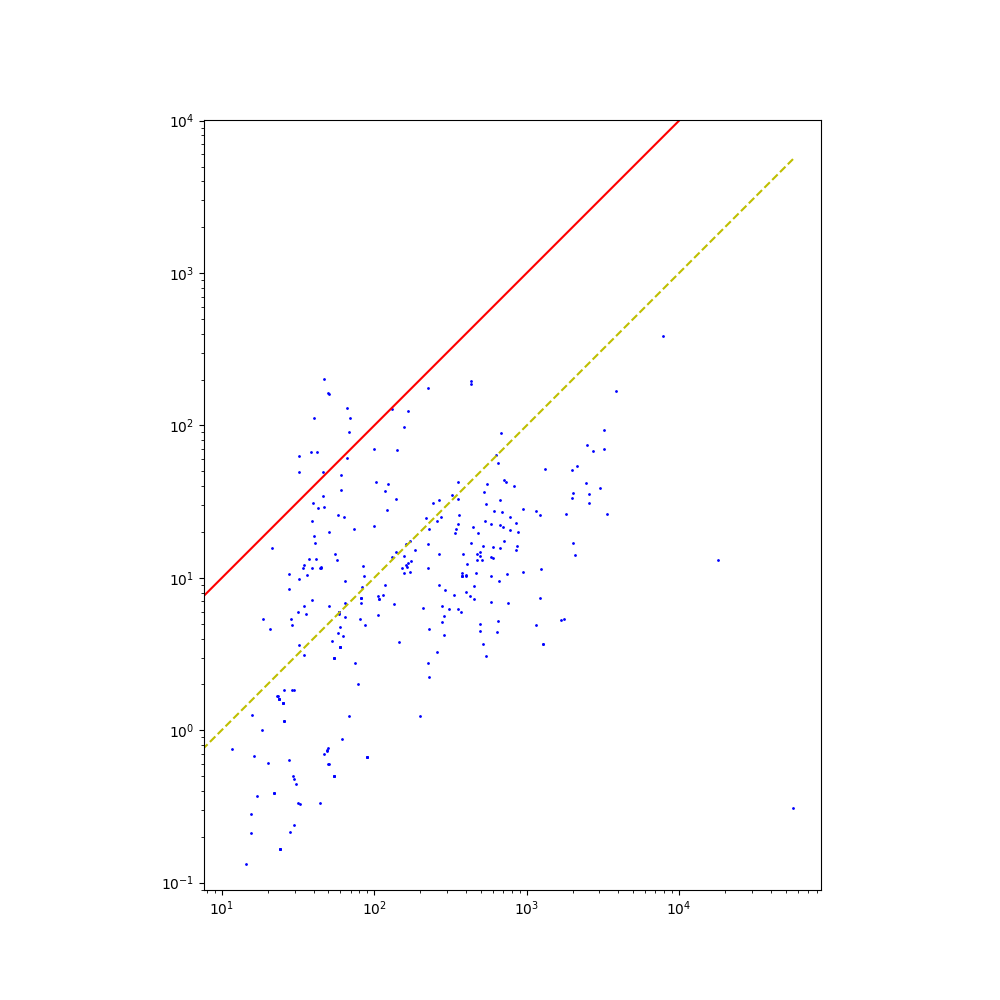
\includegraphics[width=0.35\textwidth,
                    trim=32mm 15mm 15mm 20mm] 
     {colors/gfx/normsize-no_cmemo.png}
     };
  \node(opt)[right=10mm of mono, inner sep=0] {
   \includegraphics[width=0.35\textwidth,
                    trim=32mm 15mm 20mm 20mm] 
     {colors/gfx/normsize-colored.png}
     };
  \node[below=-1mm of mono] {\axislab{separate e-graphs}};
  \node[left=-3mm of mono, rotate=90, anchor=south] {\axislab{monochrome colored e-graphs}};
  \node[below=-1mm of opt] {\axislab{separate e-graphs}};
  \node[left=-3mm of opt, rotate=90, anchor=south] {\axislab{optimized colored e-graphs}};
  \node(a)[right=10mm of opt] {$\times 1$};
  \node(b)[below=10mm of a.west,anchor=west] {$\times 10$};
  \draw[red,line width=0.8pt] (a.west) -- ++(-1, 0);
  \draw[yellow!50!gray,line width=1pt,dash pattern=on 2pt off 1pt] (b.west) -- ++(-1, 0);
\end{tikzpicture}
  %\includegraphics[width=0.3\textwidth]{gfx/normsize-colored.png}
  %\end{tabular}
  \vspace{-1em}
  \caption{Size comparison: relative e-node overhead in clones \vs color e-graph variants.}
  \label{fig:normalizedsize}
  \vspace{0.5em}
\end{figure*}

In our setup, all assumptions emerge from case splits done by the prover.
We filter out cases where no case splits were applied, since these have no assumptions introduced and thus colored e-graphs have no impact.

For each benchmark instance, we measure the \emph{relative e-node overhead} as the number of additional e-nodes that are required, normalized by the number of different assumptions.
That is, $(|\textrm{total e-nodes}| - |\textrm{base e-nodes}|) / |\textrm{assumptions}|$.
``Base e-nodes'' represent the contents of the graph before case splits.
(For the monochrome colored e-graph we use the base e-nodes present in the separate e-graphs case.)
\autoref{fig:normalizedsize} summarizes the results, pitting colored e-graphs (with and without colored e-nodes) against the baseline of separate clones.
In some cases one configuration times out or runs out of memory, while the other does not;
we only compare cases where both configurations finished the run successfully.
In both comparisons, we see roughly around 10$\times$ lower overhead, where in the monochromatic case samples are more dispersed around the y axis, and the optimized case shows clear advantage to the colored e-graph implementation.


Run-time is measured as the the total run-time for completed test cases, and 1 hour for cases that timed out.
We do not include runs that did not finish due to out-of-memory exceptions (we report the latter separately).
As can be seen in \autoref{fig:runtime}, the monochrome colored e-graph lead to many timeouts,
whereas the optimized case exhibits running times similar to separate clones.
This is in line with our expectation:
colors provide lower memory sizes at the expense of run-time.

\begin{figure*}
  \centering
  \newcommand\axislab[1]{\fontsize{7pt}{9pt}\selectfont{#1}}
\begin{tikzpicture}
  \node(mono)[inner sep=0] {
   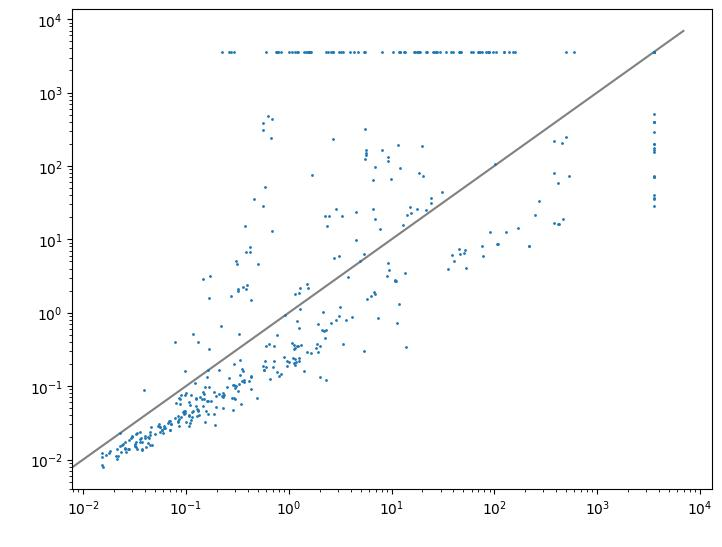
\includegraphics[width=0.35\textwidth, trim=20 20 20 15] 
     {colors/gfx/runtime-no_cmemo.jpg}
     };
  \node(opt)[right=12mm of mono, inner sep=0] {
   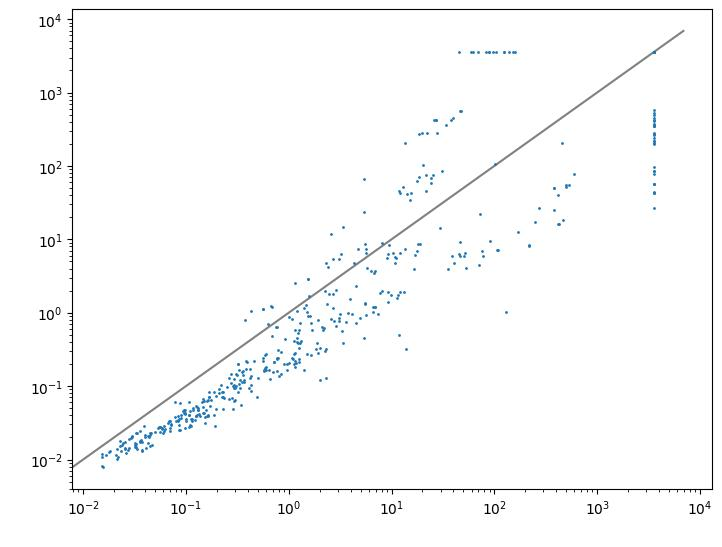
\includegraphics[width=0.35\textwidth, trim=20 20 20 15] 
     {colors/gfx/runtime-colored.jpg}
     };
  \node[below=0mm of mono] {\axislab{separate e-graphs}};
  \node[left=0mm of mono, rotate=90, anchor=south] {\axislab{monochrome colored e-graphs}};
  \node[below=0mm of opt] {\axislab{separate e-graphs}};
  \node[left=0mm of opt, rotate=90, anchor=south] {\axislab{optimized colored e-graphs}};
\end{tikzpicture}
    \vspace{-1em}
    \caption{Run-time comparison: run-time of clones vs. color e-graphs}
    \label{fig:runtime}
\end{figure*}

Finally, in \autoref{tab:runtimesuite} we present the number of out-of-memory exceptions, the number of timeout exceptions, and total run-time for each configurations and test suite.
The monochrome colored e-graph, as expected, exhibits many timeouts. 
Even though it has more errors than the other e-graph versions, it still has much longer run-times.

The optimized e-graphs demonstrate enhancements over separate e-graphs in both run-time and success rate, as detailed in \autoref{tab:runtimesuite}. 
Notably, the optimized configuration completed more tests (99 failures compared to 114). 
A key shift observed is the replacement of out-of-memory errors with timeouts, particularly in the \funcname{leon-amortize-queue} suite. 
However, \funcname{leon-heap} posed challenges for colored e-graphs, incurring 13 extra timeouts even in the optimized version. 
Conversely, the \funcname{isaplanner} suite showed a notable improvement, halving the failure rate in the optimized version compared to the baseline.

% I have a problem in how I test this, because it requires to assert both cases finished running and I can't do that at the moment
\begin{comment}
The \funcname{isaplanner} test suite contains a similar disparity, where for 79 test cases the colored e-graph has more assumptions by the end of the run.
There are no cases in \funcname{isaplanner} where the colored e-graphs had fewer assumptions, and there are only 4 test cases for which colored e-graphs had more assumptions in \funcname{leon-heap}, and none in which it had fewer.
\end{comment}


\begin{table}[t]
    \centering
    \caption{Run-time and exceptions. M = Out of memory, T = Timeout (3600) }
    \label{tab:runtimesuite}
    \setlength{\tabcolsep}{3pt} % Adjust the space between columns
    \newcolumntype{d}[1]{D{/}{/}{#1}} % New column type for O/T column
    \begin{tabular}{lrd{3}rd{3}rd{3}}
    \toprule
    & \multicolumn{2}{c}{Separate} & \multicolumn{2}{c}{Monochrome} & \multicolumn{2}{c}{Optimized} \\
    \cmidrule(r){2-3} \cmidrule(lr){4-5} \cmidrule(l){6-7}
    Test Suite & \multicolumn{1}{c}{Time} & \multicolumn{1}{l}{M/T} & \multicolumn{1}{r}{Time} & \multicolumn{1}{l}{M/T} & \multicolumn{1}{r}{Time} & \multicolumn{1}{l}{M/T} \\
    \midrule
    clam & 70.1 & 0/0 & 277.8 & 0/5 & 23.6 & 0/0 \\
    hipspec-rev-equiv & 34.1 & 0/0 & 139.0 & 0/17 & 57.0 & 0/0 \\
    hipspec-rotate & 3880.3 & 1/1 & 1871.4 & 0/6 & 17.4 & 0/3 \\
    isaplanner & 8454.4 & 0/60 & 6068.4 & 0/70 & 20486.3 & 3/28 \\
    leon-amortize-queue & 187356.4 & 52/0 & 14.8 & 0/57 & 10854.3 & 3/49 \\
    leon-heap & 1735.9 & 0/0 & 1201.8 & 0/25 & 4949.2 & 0/13 \\
    \bottomrule
    \end{tabular}
\end{table}







\begin{comment}
    \begin{tabular}{llr}
\toprule
 &  & Time \\
E-graph Type & Test Suite &  \\
\midrule
\multirow[t]{7}{*}{Seperate e-graphs} & clam & 34.234764 \\
 & hipspec-nichomachus & 0.050861 \\
 & hipspec-rev-equiv & 2.577174 \\
 & hipspec-rotate & 237.717540 \\
 & isaplanner & 8913.695004 \\
 & leon-amortize-queue & 9.668328 \\
 & leon-heap & 216.857437 \\
\cline{1-3}
\multirow[t]{7}{*}{Monochromatic colored e-graphs} & clam & 394.891332 \\
 & hipspec-nichomachus & 0.087772 \\
 & hipspec-rev-equiv & 0.720120 \\
 & hipspec-rotate & 1970.451256 \\
 & isaplanner & 1739.190107 \\
 & leon-amortize-queue & 0.294397 \\
 & leon-heap & 1206.035020 \\
\cline{1-3}
\multirow[t]{7}{*}{Optimized colored e-graphs} & clam & 6.049511 \\
 & hipspec-nichomachus & 0.085397 \\
 & hipspec-rev-equiv & 42.016671 \\
 & hipspec-rotate & 78.174158 \\
 & isaplanner & 12337.053032 \\
 & leon-amortize-queue & 43.787478 \\
 & leon-heap & 791.375722 \\
\cline{1-3}
\bottomrule
\end{tabular}
\end{comment}
\section{Related Work}
\label{colors:related}

\myparagraph{Theory exploration and its applications.}
Interest in exploratory reasoning in the context of functional calculi started with IsaCoSy~\cite{JAR2010:Johanssonisacosy}, a system for lemma discovery based in part on CEGIS~\cite{ASPLOS2006/Solar-Lezama}.
In a seminal paper, QuickSpec~\cite{JFP2017:Smallbone}
propelled applicability of such reasoning for inferring specifications from implementations
based on random testing,
with deductive reasoning to verify generated conjectures~\cite{ICAD2013:Claessen,ITP2017:Johansson}.
TheSy~\cite{thesy} and Ruler~\cite{ruler} have both incorporated e-graphs to some extent in the exploration process: they are used to speed up equivalence reduction of the space of generated terms, and, in~\cite{thesy}, also the filtering and qualification phases using symbolic examples.
The evaluation of the latter shows quite clearly that case splitting is a major obstacle to symbolic exploratory reasoning,
due to the large number of different cases and derived assumptions.

In the area of conditional rewrite discovery,
Speculate~\cite{speculate}
naturally builds on the techniques from QuickSpec and depends on property-based testing techniques to generate inputs that satisfy some conditions.
SWAPPER~\cite{DBLP:conf/fmcad/0002S16} is a relatively early example of exploring using SyGuS with a data-driven inductive-synthesis approach with emphasis on finding rules that are most efficient for different problem domains.
It requires a large corpus of similar SMT problems to operate.

%QuickSpec etc (from TheSy and others), Ruler, SWAPPER, Speculate, Spectacular
%Case splitting in hipspec and conditions in Speculate

\myparagraph{Other e-graph extensions.}
E-graphs were originally brought into use for automated theorem proving~\cite{JACM2005:Detlefs},
and were later popularized as a mechanism for implementing low-level compiler
optimizations~\cite{POPL2009:Tate},
by extending them with ``$\varphi$-nodes'' to express loops.
Relational e-matching~\cite{DBLP:journals/pacmpl/ZhangWWT22}
makes use of Datalog semina\"ive evaluation
to harness the power of query planning in database systems.
Subsequently, Datalog-powered e-matching has been recently fused with core Datalog semantics to allow richer logic programming by exposing equality saturation as a building block in a framework called egglog~\cite{DBLP:pldi23/Zhang}.
Since Datalog is based on Horn clauses, this meshes very well with conditional rewriting.
It should be noted, though, that it is still a monotone framework, and does not allow backtracking or simultaneous exploration of alternative assumptions.

ECTAs~\cite{Koppel22,Koppel23} are another, related compact data structure that extends e-graphs, Version-Space Algebras~\cite{DBLP:conf/icml/LauDW00,DBLP:journals/ml/LauWDW03}, and Finite Tree Automata~\cite{DBLP:journals/pacmpl/0001M17},
with the concept of ``entanglement'';
that is, some choices of terms from e-classes
may depend on choices done in other e-classes.
Since the backbone of ECTAs is quite similar to an e-graph, the colors extension is applicable to this domain as well.

\myparagraph{Uses of e-graphs in SMT.}
E-graphs are a core component for equality reasoning in SMT solvers~\cite{z3,DBLP:conf/tacas/BarbosaBBKLMMMN22}, in most theory solvers such as QF\_UF, linear algebra, and bit-vectors.
E-matching is also used for quantifier instantiation~\cite{DBLP:conf/tacas/NiemetzPRBT21}, which is, in its essence, an exploratory task and requires efficient methods~\cite{DBLP:conf/cade/MouraB07}.
In these contexts, implications and other Boolean structures are treated by the SAT core (in CDCL(T)), and the theory solver only handles conjunctions of literals.

\section{Conclusion}
\label{colors:conclusions}
% We created colored e-graphs for multiple congruence relations
% We evaluated and it is good


% We want future work


\begin{comment}
In conclusion, this paper has introduced the concept of colored e-graphs as a memory-efficient method for maintaining multiple congruence relations in a single e-graph. 
It provides support for equality saturation with additional assumptions over e-graphs, thereby enabling efficient exploratory reasoning of multiple assumptions simultaneously.
The development of several optimizations based on the egg library and deferred rebuilding, and subsequent evaluation has validated our approach, demonstrating a significant improvement in memory utilization and a modest one for run-time performance compared to the baseline.
\end{comment}

We presented colored e-graphs as an approach to efficiently handle multiple congruence relations in a single e-graph.
They provide a memory-efficient method for equality saturation with additional assumptions, crucial for efficient exploratory reasoning of multiple assumptions simultaneously.
Our optimizations, developed using the egg library, have shown notable improvements in memory usage and moderate enhancements in run-time performance over the baseline.

%This work thus serves as a stepping stone, advancing the current state of the art and setting a foundation for works on exploratory reasoning tools and techniques. 
%By extending e-graph capabilities, we hope to drive new innovation in the realm of symbolic reasoning and its applications.
\chapter{Lightweight Equality Saturation for Proof Assistants}
\label{chap:lw-eqsat}

\section{Introduction}

Proof assistants have become increasingly important tools in formalization of mathematics, formal verification, and program analysis. 
The have become indispensable in tasks such as verification of complex systems, that require a high level of expressivity \cite{bedrock, compcert}.
However, their usability depends on an expert user being able to select the appropriate proof steps within the interactive environment.
Users can take advantage of automation features provided by the proof assistant, but this requires a higher level of skill~\cite{qedatlarge}.

Researchers recently had substantial success in using automated theorem proving (ATP) as a component in interactive theorem provers (ITPs, often referred to as proof assistants).
An ATP can be a useful automatic one click solution to the vast amount of effort put into verifying software using ITPs \cite{qedatlarge,compcert,bedrock}.
However, ATPs usually reason over first order logic (FOL), and proof assistants use a more expressive high order logic (HOL), requiring an encoding of the proof assistants environment into FOL.
This is usually done by tools called \emph{hammers}, and for the ATPs to be effective, requires facts (axioms and lemmas) selection mechanism, as too many axioms will often make the proof search diverge \cite{coqhammer, hammeringqed, sledgehammer}.

Despite their effectiveness in certain scenarios, hammers present significant limitations in terms of interactivity within proof assistants.
A key issue that when a hammer fails to prove a theorem, it offers no insights into why the proof attempt was unsuccessful or how the user might proceed. 
This lack of intermediate feedback is particularly problematic in interactive theorem proving environments, where users often require guidance to refine their proof strategies or identify missing lemmas.
This limitation restricts the ability of expert users to effectively guide the proof process in complex scenarios where automated methods alone are insufficient.

\begin{comment}
This chapter introduces an approach dubbed Lightweight Equality Saturation (LES) for proof assistants, which aims to apply equality saturation to a reduced form of the available theory, thus maintaining computational efficiency required for an interactive setting.
By selectively applying saturation techniques to critical subterms and leveraging domain-specific heuristics, LES offers a promising framework for enhancing the capabilities of proof assistants without incurring prohibitive performance costs.
\end{comment}

This chapter introduces an approach called Lightweight Equality Saturation (LES) for proof assistants, which aims to somewhat bridge the gap between automated theorem proving and interactive proof environments. 
LES leverages the power of equality saturation \cite{eqsat}, a technique to effectively reason about equality of terms, through an the ITPs hammer mechanisms.
Equality saturation operates by repeatedly, and simultaneously, applying rewrite rules on top of an e-graph \cite{egg}, a data structure that compactly represents equivalence classes of expressions. 
By employing a smart encoding to an e-graph and carefully constructed rewrite rules, LES achieves a balance between speed and effectiveness as a prover.

A key advantage of the LES approach is its ability to potentially provide meaningful feedback even when it fails to prove a theorem completely. 
In such cases, LES can attempt to offer a simplified sub-goal that, if proven, would enable the proof of the full goal. 
This can significantly enhances the interactive experience, allowing users to make incremental progress and gain insights into the proof structure. 
It's important to note that an eqsat-based prover like LES has inherent limitations: it struggles with existential quantification and lacks built-in mechanisms for case splitting or induction. 
However, these limitations are well-suited to the ITP scenario, where a rich ecosystem of existing lemmas often already addresses case reasoning or induction steps.
To ensure successful application and maintain efficiency, the LES translation process incorporates several crucial optimizations. 
Given that e-graphs are sensitive to size due to the exponential nature of e-matching (the basis for rewriting in equality saturation), the translation carefully avoids introducing unnecessary terms into the e-graph. 
Furthermore, LES implements special refinements for handling equality, if-and-only-if statements, and propositions, making it particularly well-suited for pure type systems commonly used in proof assistants.
But, to keep the prover fast, no attempts to deal with existentials or conditionals are made.
Still, the prover manages to go toe-to-toe with state of the art theorem provers, and improve CoqHammer's overall results.

The main contributions of this work are threefold. 
\begin{enumerate}
    \item We present LES, a novel implementation of Lightweight Equality Saturation for Coq.
    \item We introduce a tool that leverages Coq-LSP, a language server protocol meant to replace \cite{serapi} to facilitate the easy creation of benchmarks. 
    This tool significantly streamlines the process of generating and managing test cases for any coq tactic, enabling more comprehensive and efficient evaluation of proof automation techniques.
    \item We provide an evaluation of LES on the MathComp coq library, comparing its performance against existing automated reasoning tools, cvc4 \cite{cvc4}, vampire \cite{vampire}, z3 \cite{z3}, and the E prover \cite{eprover}, and assessing its impact on CoqHammer \cite{coqhammer}. 
    This evaluation demonstrates the effectiveness of our approach. Also an ablation study is done to asses the effectiveness of a critical encoding design choice on the effectiveness of the LES prover.
\end{enumerate}  

% Even when solvable by tactics, requires experts
% This is expensive because assholes like Eytan ask for big salaries
% Automatic tools that will allow non-experts to handle this french piece of shit, often fail, and provide no help
\section{Background}
\label{lweqsat:background}

Proof assistants usually consist of two basic layers: a \emph{kernel} is responsible for checking proofs, and some user facing scripting language, commonly called a \emph{tactic language} that is used to ease and streamline the construction of proof objects that are passed to the kernel for checking.
This split is conducive to the evolution of proof assistants, because the tactics can be developed more flexibly, without worrying about proof soundness.
The kernel alone forms the TCB (trusted code base) that is assumed correct.

Two of the most commonly used proof assistants today, Coq and Lean \ES{cite}, are based on Type Theory, thus reducing the problem of proof checking to one of \emph{type checking}.
They employ similar flavors of the Calculus of Inductive Constructions (CIC), which is a typed pure lambda calculus with polymorphism and, importantly, dependent types.
In such calculi, types are first-class expressions, and 
type checking relies heavily on syntactic unification of terms.
To offer some automatic assistance, terms are reduced to a \emph{normal form} and then compared.
The normalization relies on the set of reductions that are part of the calculus (the most basic ones being $\beta$-reduction and $\eta$-reduction),
as well as on definitions of basic mathematical concepts that are used (such as arithmetic operators like $+$ and $\cdot\,$).

%(modulo $\beta$-equivalence).
%Terms that are not syntactically identical but are nevertheless semantically equivalent, such as $x\cdot 5$ and $5\cdot x$, require manual application of the tactic language to show equality.

\subsection{Hammer Systems}

Hammer systems have emerged as powerful tools for automating proof discovery in ITPs. These systems typically combine premise selection, translation to first-order logic, and proof reconstruction. Notable examples include Sledgehammer for Isabelle/HOL \cite{sledgehammer}, HOLyHammer for HOL Light \cite{holyhammer}, and CoqHammer for Coq \cite{coqhammer}. These systems have demonstrated significant success in automatically proving a substantial portion of theorems in their respective libraries.

\subsection{Translations to First-Order Logic}

A key component of hammer systems is the translation of higher-order or dependently typed logics to first-order logic. This translation enables the use of highly optimized automated theorem provers (ATPs) that operate on first-order logic. Significant work in this area includes:

\begin{itemize}
    \item Czajka's shallow embedding of pure type systems into first-order logic \cite{czajka2018shallow}, which provides a foundation for translating dependently typed systems.
    \item Meng and Paulson's technique for translating higher-order clauses to first-order clauses \cite{meng2008translating}, which has been influential in the development of hammer systems for higher-order logic.
\end{itemize}

These translations face the challenge of balancing completeness, soundness, and practical efficiency.

\subsection{Automation in Dependently Typed Systems}

Dependently typed proof assistants like Coq and Lean have their own built-in automation tactics. Coq provides tactics such as \texttt{auto}, \texttt{eauto}, and \texttt{firstorder} \cite{Coq:manual}, which perform limited proof search. Lean offers a powerful tactic framework that allows users to write custom automation \cite{lean}.

Integration with SMT solvers has also been explored, as exemplified by Armand et al's work \cite{armand2011modular}, which integrates SMT solvers into Coq's by using proof witnesses, as opposed to hammers which attempt to reconstruct proofs using deductions.

\subsection{Premise Selection}

Efficient premise selection is crucial for the performance of hammer systems, especially when dealing with large formal libraries. Recent advancements in this area include the use of machine learning techniques. For instance, \ES{TODO}.

\subsection{Equality Saturation}

Equality saturation, implemented efficiently using e-graphs, has shown promise in program optimization and equivalence reasoning \cite{egg}. This technique allows for a more flexible exploration of the equality relation, potentially offering advantages in proof search and simplification.

Our work builds upon these foundations, aiming to develop a lightweight equality saturation approach for Coq that balances automation power with logical soundness and efficiency.
\chapter{Conclusion and Future Directions}
\label{chap:conclusion}

This thesis has explored the application of equality saturation techniques to enhance automatic deductive reasoning across various domains.
We have developed novel approaches that address key challenges in this field.

The first basic challenge we faced when attempting to create automatic deduction tools, was incomplete background theory. 
Deductive reasoning is limited by the background theory, and thus the problem of an incomplete one needed addressing.
TheSy (presented in \autoref{chap:thesy}), our symbolic theory exploration system, represents a significant advancement in the field of theory exploration.
By leveraging equality saturation techniques, TheSy efficiently discovers and proves new lemmas in mathematical theories. 

Our experiments demonstrated that TheSy can discover a broader knowledge base than previous testing-based approaches while being faster in most cases. 
This efficiency gain is particularly pronounced when dealing with complex data types and function compositions, where concrete testing methods often struggle.

One significant issue encountered with TheSy was trying to perform conditional reasoning in combination with equality saturation.
Existing solutions provide either mechanisms to have some local conditional reasoning, or create a copy of the underlying e-graph leading to higher memory consumption.
To address this challenge within the equality saturation framework, we introduced colored e-graphs (presented in \autoref{chap:colors}).
This novel extension to e-graphs provides a memory-efficient and flexible approach to representing multiple equality relations within a single structure. Key features of colored e-graphs include:
A layered approach to representing multiple congruence relations, with each layer corresponding to a specific condition or assumption;
efficient sharing of common substructures, reducing memory overhead;
specialized algorithms for merging, rebuilding, and e-matching operations that take advantage of the layered structure.

Our evaluation showed that Colored E-graphs can significantly reduce memory usage compared to maintaining separate e-graphs for different conditions, while maintaining similar runtime performance. 
This advancement opens new possibilities for applying equality saturation techniques to problems involving complex conditional reasoning.

Even though we presented solutions for basic problems encountered in automated deductive reasoning, and specifically in equality saturation, the challenge of applying equality saturation as a theorem prover remained.
The main advantage of the equality saturation approach is in its ability to deal with a huge background theory, but it suffers from no other builtin reasoning techniques, limiting it to the said background theory.
Thus, we developed the Lightweight Equality Saturation (LES) prover in the domain of interactive theorem proving (presented in \autoref{chap:les}).
In the context of interactive theorem proving, applying automatic theorem provers is considered difficult due to the vast amount of available lemmas and theorems.
LES bridges the gap between automated reasoning and interactive proof assistants by providing a fast, automated reasoning tool that integrates well with interactive environments. 

Our experiments with LES showed promising results in automatically proving theorems within the Coq proof assistant, demonstrating its potential to enhance the capabilities of ITPs.
Even though, there are still many open directions to enhance it's capabilities.

\section{Open Questions and Future Directions}

While our work has made significant strides in applying equality saturation to automatic deductive reasoning, several important questions and research directions remain open for future exploration:

A key challenge for future research is to extend symbolic theory exploration to efficiently discover conditional lemmas. 
For example, can we use colored e-graphs to find lemmas such as a sorted list is increasing? 
This presents challenges in both scale and discovery of conditions and lemmas.
The potential of colored e-graphs opens up several directions for exploring their effectiveness in other tasks, such as global program optimizations or symbolic execution, hopefully leading to new state-of-the-art discoveries.

Although LES is an effective prover, several direction for future studies remain. 
Extending it with conditional and inductive reasoning using colored e-graphs could significantly improve its ability.
Also, due to it's interactive design, LES has the potential to serve as a deductive reasoning framework for agents, whether human or artificial, that would direct difficult to automate procedures such as case splitting, induction, and existential variables instantiation.

\section{Closing Remarks}

The work presented in this thesis address key challenges in theory exploration, conditional reasoning, and integration with interactive theorem provers, and have opened new avenues for research in automated reasoning.

The three components presented, TheSy, colored e-graphs, and LES, synergize to create a thorough approach to improving the applicability of automatic deductive reasoning.
TheSy's ability to efficiently discover new lemmas provides a richer knowledge base, which LES can leverage to handle complex reasoning scenarios.
Also, colored e-graphs for conditional reasoning can potentially imporve theory exploration systems and theorem provers based on equality saturation. 
These innovations form a potent toolkit that addresses key challenges in automated reasoning.

We hope these insights and innovations will further advance automatic deductive reasoning, bringing creating effective and autonomous reasoning agents that will help in a wide range of domains.
%
% Add any appendices here; they must come _before_ the bibliography
%
\appendix
%\noappendicestocpagenum
%\addappheadtotoc
\chapter{Algorithms Pseudo Code}
\label{app:algorithms}

Colored e-graphs introduce a few algorithmic changes to the operations of a normal e-graph.
Here we present pseudo code for the important changes presented in the paper.
Algorithms \ref{alg:compare} and \ref{alg:colored_jump} present the changes being made to the e-matching abstract machine to support \emph{unoptimized} colored e-matching as presented in \autoref{colors:functional}.

\begin{algorithm}
\caption{Function: compare}
\label{alg:compare}
\begin{algorithmic}
\STATE \textbf{Input:} $i$, $j$
\IF{$find(color, reg[i]) \neq find(color, reg[j])$}
    \STATE \textbf{backtrack}
\ENDIF
\end{algorithmic}
\end{algorithm}

\begin{algorithm}
\caption{Function: colored\_jump}
\label{alg:colored_jump}
\begin{algorithmic}
\STATE \textbf{Input:} $i$
\STATE $siblings \gets \{e | e \in E \land e \equiv_{color} eclass\}$
\FOR{$sibling$ in $siblings$}
    \STATE $reg[i] = sibling$
    \STATE $bs$.push(current\_state)
\ENDFOR
\STATE \textbf{backtrack}
\end{algorithmic}
\end{algorithm}

The rebuilding algorithm is also updated to accommodate for colored e-graphs in \autoref{colors:functional}.
We update the auxiliary function \textsc{repair} to work on colored e-classes,
and introduce two new helper functions: $\textsc{collect\_parents}$ and $\textsc{update\_hashcons}$, as presented in Algorithms \ref{alg:rebuild}, \ref{alg:repair}, \ref{alg:update_hashcons}, and \ref{alg:collect_parents}.
$\textsc{collect\_parents}$ extract the parents of a colored e-class by combining the sets of parents of all the (root) e-classes contained therein.
$\textsc{update\_hashcons}$ is used to make sure that the hashcons entries are in canonical forms. It was already a part of \textsc{repair} in egg;
it is only repeated here to point out that it
only updates the hashcons for the root color,
since no canonization is required for colored layers.    

\begin{algorithm}
\caption{Function: rebuild}
\label{alg:rebuild}
\begin{algorithmic}
\FOR{$color$ in $self.colors$}
    \WHILE{$self.worklist(color).len() > 0$}
        \STATE $todo \gets$ TAKE($self.worklist(color)$)
        \STATE $todo \gets \{ self.find(color, eclass) | eclass \in todo \}$
        \FOR{each $eclass$ in $todo$}
            \STATE CALL $self.repair(color, eclass)$
        \ENDFOR
    \ENDWHILE
\ENDFOR
\end{algorithmic}
\end{algorithm}

\begin{algorithm}
\caption{Function: repair}
\label{alg:repair}
\begin{algorithmic}
\STATE \textbf{Input:} $color$, $eclass$
\STATE $parents \gets$ CALL collect\_parents($color, eclass$)
\STATE CALL update\_hashcons($color, parents$)
\STATE $new\_parents \gets \{\}$
\FOR{each $(p\_node, p\_eclass)$ in $parents$}
    \STATE $p\_node \gets self.canonicalize(color, p\_node)$
    \IF{$p\_node$ is in $new\_parents$}
        \STATE $self.merge(color, p\_eclass, new\_parents[p\_node])$
        \STATE $new\_parents[p\_node] \gets self.find(color, p\_eclass)$
    \ENDIF
\ENDFOR
\IF{$color = root$}
    \STATE $eclass.parents \gets new\_parents$
\ENDIF
\end{algorithmic}
\end{algorithm}

\begin{algorithm}
\caption{Function: update\_hashcons}
\label{alg:update_hashcons}
\begin{algorithmic}
\STATE \textbf{Input:} $color$, $parents$
\IF{$color = root$}
\FOR{each $(p\_node, p\_eclass)$ in $parents$}
    \STATE $self.hashcons.remove(p\_node)$
    \STATE $p\_node \gets self.canonicalize(color, p\_node)$
    \STATE $self.hashcons[p\_node] \gets self.find(color, p\_eclass)$
\ENDFOR
\ENDIF
\end{algorithmic}
\end{algorithm}

\begin{algorithm}
\caption{Function: collect\_parents}
\label{alg:collect_parents}
\begin{algorithmic}
\STATE \textbf{Input:} $color$, $eclass$
\STATE $all\_parents \gets \emptyset$
\STATE $relevant\_eclasses \gets \{e | e \in E \land e \equiv_{color} eclass\}$
\FOR{$e$ in $relevant\_eclasses$}
    \STATE $all\_parents \gets all\_parents \cup e.parents$
\ENDFOR
\STATE return $all\_parents$
\end{algorithmic}
\end{algorithm}

The pseudo code for the optimized e-matching instructions that were presented in \autoref{colors:optimizations} are presented in Algorithms \ref{alg:compare_optimized} and \ref{alg:colored_jump_optimized}.

\begin{algorithm}
\caption{Function: compare' (optimized)}
\label{alg:compare_optimized}
\begin{algorithmic}
\STATE \textbf{Input:} $i$, $j$
\IF{$find(color, reg[i]) \neq find(color, reg[j])$}
    \STATE $descendants \gets \{ c | color \in p^+(c) \land reg[i] \equiv_c reg[j] \}$
    \STATE $minimal \gets \{ c | c \in descendants \land \lnot \exists c' \in descendants. c' \in p^+(c) \}$
    \FOR{$c$ in $minimal$}
        \STATE $color = c$
        \STATE $bs$.push(current\_state)
    \ENDFOR
    \STATE \textbf{backtrack}
\ENDIF
\end{algorithmic}
\end{algorithm}

\begin{algorithm}
\caption{Function: colored\_jump' (optimized)}
\label{alg:colored_jump_optimized}
\begin{algorithmic}
\STATE \textbf{Input:} $i$
\STATE $siblings \gets \{e | e \in E \land e \equiv_{color} eclass\}$
\FOR{$sibling$ in $siblings$}
    \STATE $reg[i] = sibling$
    \STATE $bs$.push(current\_state)
\ENDFOR
\STATE $descendants \gets \{ (c, e) | color \in p^+(c) \land reg[i] \equiv_c e \land e \notin siblings \}$
\STATE $minimal \gets \{ (c, e) | (c, e) \in descendants \land \lnot \exists (c', e') \in descendants. (c' \in p^+(c) \land e' \equiv_c' e) \}$
\FOR{$(c,e)$ in $minimal$}
    \STATE $color = c$
    \STATE $reg[i] = e$
    \STATE $bs$.push(current\_state)
\ENDFOR
\STATE \textbf{backtrack}
\end{algorithmic}
\end{algorithm}

\begin{comment}

\chapter{Some sort of an appendix}
\label{appendix:somesort}

You may want to include appendices of your own volition. Also, if you've developed any computer software, that needs to go in as an appendix as well.

\section{A first section in this appendix}

Some appendix content here. And something nice to finish things off:

\begin{figure}[htb]
  \centering
  \ifpdf
    \includegraphics[width=0.3\textwidth]{graphics/mygraphic2.png}
  \else
    \includegraphics[width=0.3\textwidth]{graphics/mygraphic2-for-ps.eps}
  \fi
  \caption{A Flower.}
\end{figure}

\section{Another appendix section}
After the (last) appendix-section comes the thesis' bibliography; Its style is set with the \verb|\thesisbibstyle| command. Then there are the Hebrew parts of thesis, which don't exactly ``follow" the bibliography in a logical sense, but rather start at the beginning of the thesis when considered as a right-to-left printed booklet. Thus, the last page of the extended Hebrew abstract of the thesis comes right ``after" the last page of the bibliography if you're turning the pages in left-to-right order.

\end{comment}

% Back Matter
% ------------

% The following command will typeset the bibliography,
% then typeset the Hebrew part of the thesis:
% - Cover page
% - Title page
% - Acknowledgements page
%  (NO table of contents or list of figures in Hebrew)
% - (Extended) abstract (1000-2000 words)
%
% based on information you've provided in the thesis-fields file
% (including the relative paths to your bib files). The Hebrew
% content will be typeset in _reverse_page_order_, i.e. first
% in the file will be the last page of the abstract, and the
% Hebrew cover page will be the last page of the file.
%
\makebackmatter

% The resulting PDF can be printed and taken straight to binding,
% i.e. you do not need to flip any pages anywhere. Of course,
% mind the LaTeX error and warning messages, overfull hboxes etc.

\end{document}

